\chapter{MODELAGEM E PROCESSAMENTO SÍSMICO}
\label{cap.2}

O método sísmico de reflexão, consiste, basicamente, em obter informações da subsuperfície através da propagação de ondas produzidas por fontes artificiais em superfície e o posterior registro dessas ondas em receptores (geofones), que estão em superfície.
As ondas geradas pelas fontes propagam-se na subsuperfície, sendo transmitidas, refletidas e difratadas por interfaces geológicas que delimitam as camadas de rochas de diferentes propriedades físicas.
As ondas registradas nos receptores são provenientes das reflexões das interfaces, o sinal registrado pelos receptores possuem informações sob as ondas propagadas e suas mudanças conforme o trajeto do percusso da onda.


O método sísmico baseia-se na propagação do campo de onda, ou seja, na evolução temporal e espacial da frente de onda através de um meio com propriedades distintas e específicas, nas quais afetam diretamente a energia sísmica em propagação, fazendo-se necessário o estudo da equação da onda para compreender os fenômenos físicos envolvidos.

O campo de onda propagado é representado através de raios, que são retas perpendiculares as frentes de ondas (esféricas) com origem na fonte sísmica (perturbação).

O que se deseja no experimento sísmico é estimativa do tempo de trânsito ($\tau$) ao longo de uma trajetória qualquer referente a pares fonte-receptor, este pode ser calculado baseada no traçamento de raios e na lei de Snell para cada interface atravessada. Neste cálculo é empregada a equação iconal (equação \ref{eq:iconal}). Esta equação depende do conhecimento da distribuição das velocidades intervalares do modelo.

\begin{equation}
(\nabla \tau)^{2}=\frac{1}{v^{2}}
\label{eq:iconal}
\end{equation}

\section{MODELAGEM DA ESTRUTURA GEOLÓGICA}

O objetivo da modelagem de uma seção sísmica é a construção de um modelo que represente a subsuperfície de forma coerente geologicamente. A modelagem sísmica pode ser feita de forma direta e inversa a primeira é realizada quando se parte de um modelo geológico ``a priori'' onde conhecendo os parâmetros (velocidade, densidade), é gerada a resposta da energia de amplitude das ondas propagadas sob a condição da geometria das interfaces e camadas, registradas no sismograma sintético. Já na modelagem inversa, tem-se a resposta sísmica da subsuperfície e a partir da resposta, tenta-se então estimar os parâmetros sísmicos para construir um modelo geológico conciso a essas propriedades estimadas.

A modelagem direta, ou seja, o processo através do qual um modelo geológico de subsuperfície, em uma, duas ou três dimensões, é transformado em um registro sísmico sintético de dimensão correspondente, foi primeiramente usado por exploracionistas na década de 50 \citep{Edwards(1988)}.

A modelagem sísmica consiste de um sistema de equações diferenciais parciais (geralmente equações da onda acústicas, elásticas, visco-elásticas, etc.) acompanhadas das condições de contorno (comportamento nas interfaces e bordas do modelo) e condições iniciais (caracterização da emissão de energia pela fonte, tempo de propagação requerido, etc.). Na modelagem acústica na ausência de fontes internas, o sistema de equações diferenciais que expressa a resposta de um modelo geológico a um campo de ondas incidente, é constituído de equações da onda do tipo:

\begin{equation}
\nabla^{2}P(\mathbf{x},t)-\frac{1}{v^{2}}\frac{\partial^{2}}{\partial t^{2}}P(\mathbf{x},t)= 0,
\label{eq:Equacao_onda_acustica_0}
\end{equation}


O pacote Seismic Unix (SU) oferece programas de modelagem e processamento de dados sísmicos. Para a modelagem da estrutura geológica foi usada o programa \textit{trimodel} do pacote SU, esta rotina se baseia na triangulação de Delaunay. Este método sofisticado de geração de gráficos e imagens digitais, em duas ou três dimensões, é amplamente utilizado para modelar
a superfície de objetos de diferentes complexidades. Foi desenvolvido em 1934 pelo matemático russo Boris Nikolaevich, e consiste em representar o objeto através de uma malha de triângulos que cumprem a condição de Delaunay: ``O interior da circunferência que circunscreve cada triângulo deve ser vazia'' \citep{Hale(1991)}.

\begin{figure}[H]
\centering
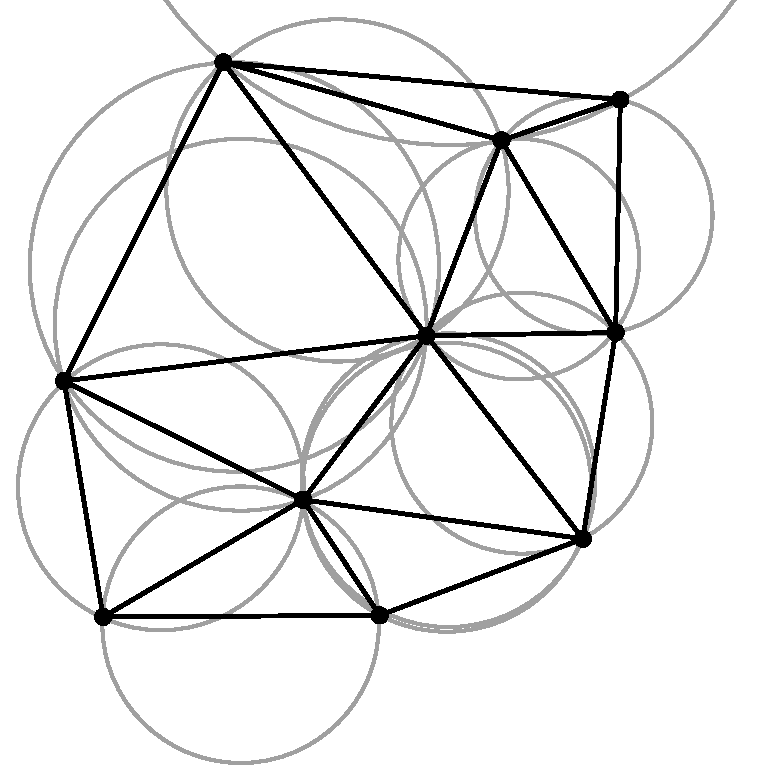
\includegraphics[width=7cm]{figuras/cap2/Delaunay_circumcircles_vectorial.pdf}
\caption{Triangulação de Delaunay no plano com as circunferências visíveis. Fonte: Wikipédia}
\label{fig:Delaunay_circumcircles_vectorial}
\end{figure}

O programa \textit{trimodel} do SU cria um modelo triangularizado, como mostra a figura (\ref{fig:vagarosidade}) a partir do modelo de velocidade da figura (\ref{fig:modelo_velocidade}). 
A velocidade é introduzida na forma de vagarosidade ($\textit{sloth}=1/v$), o método realiza o traçamento dos raios baseado na equação iconal \citep{Forel(2005)}. A vagarosidade ao quadrado das regiões (triângulos) é determinada pela equação (\ref{eq:vagarosidade}), onde o usuário define como é a variação da velocidade dentro de cada camada, na forma:

\begin{equation}
s(x,z)=s_{0}+\left(x-x_{0}\right) \frac{ds}{dx}+\left(z-z_{0}\right) \frac{ds}{dz}
\label{eq:vagarosidade}
\end{equation}

Cada par de x-z ainda é um ponto em uma camada. Na equação (\ref{eq:vagarosidade}) $x$, $x_0$, $z$ e $z_0$ são os pontos finais e iniciais na horizontal e na vertical onde ocorrerá a variação da velocidade, esta variação terá um gradiente na direção x correspondente a $ds/dx$ e na direção z de magnitude $ds/dz$.

A descrição da subsuperfície requer uma representação matemática (modelagem numérica ou modelagem sísmica), as ondas sísmicas se propagação com diferentes velocidades em subsuperfície em função dos diferentes tipos de rochas em subsuperfície. A tabela \ref{tab:tab1} apresenta os valores utilizados na construção do modelo de velocidade do modelo de camadas curvas (ver figura \ref{fig:modelo_velocidade}).

\begin{table}[H]
\centering
\begin{tabular}{|c|c|c|}
\hline
Camada & Velocidade da onda sísmica (m/s) & Vagarosidade $(m/s)^{-1}$ \\ \hline
1 & 1600 & 0.39 \\ \hline
2 & 1800 & 0.31 \\ \hline
3 & 1900 & 0.28 \\ \hline
4 & 2000 & 0.25 \\ \hline
5 & 1350 & 0.55 \\ \hline
6 & 1500 & 0.44 \\ \hline
7 & 2500 & 0.16 \\ \hline
\end{tabular}
\caption{Tabela de valores de vagarosidade e velocidade do modelo de camadas curvas.}
\label{tab:tab1}
\end{table}

\begin{landscape}
\begin{figure}[H]
\centering
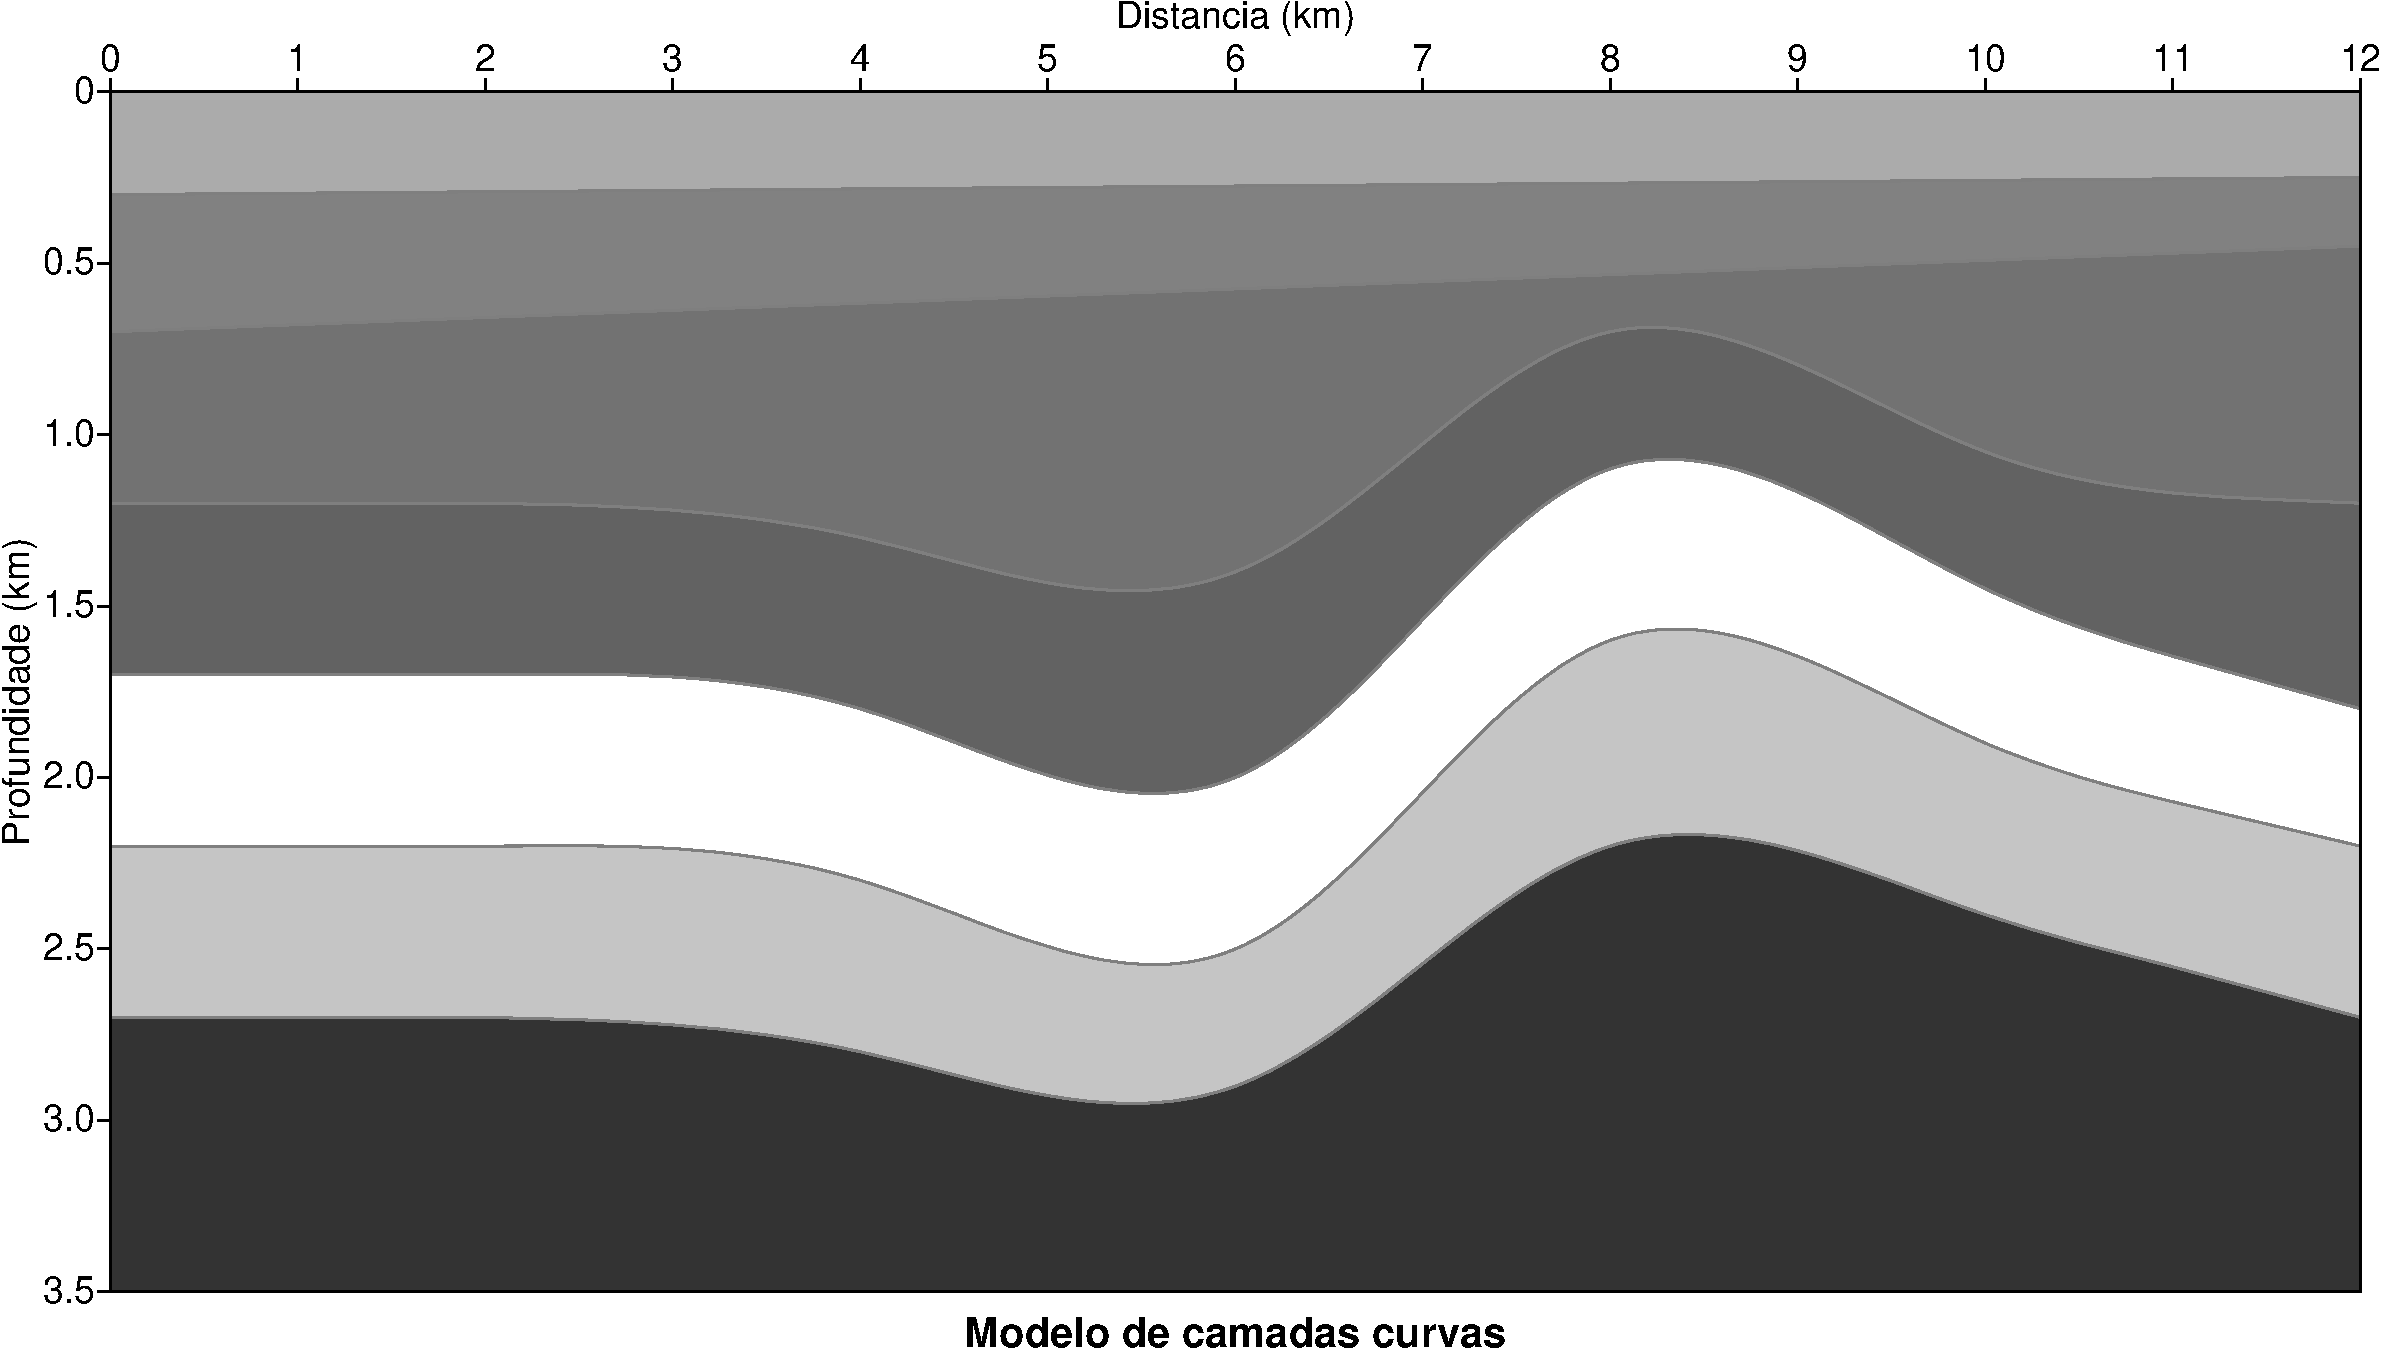
\includegraphics[totalheight=14cm]{figuras/cap2/vagarosidade.pdf}
\caption{Modelo 2D de camadas curvas.}
\label{fig:vagarosidade}
\end{figure}
\end{landscape}

\begin{landscape}
\begin{figure}[H]
\centering
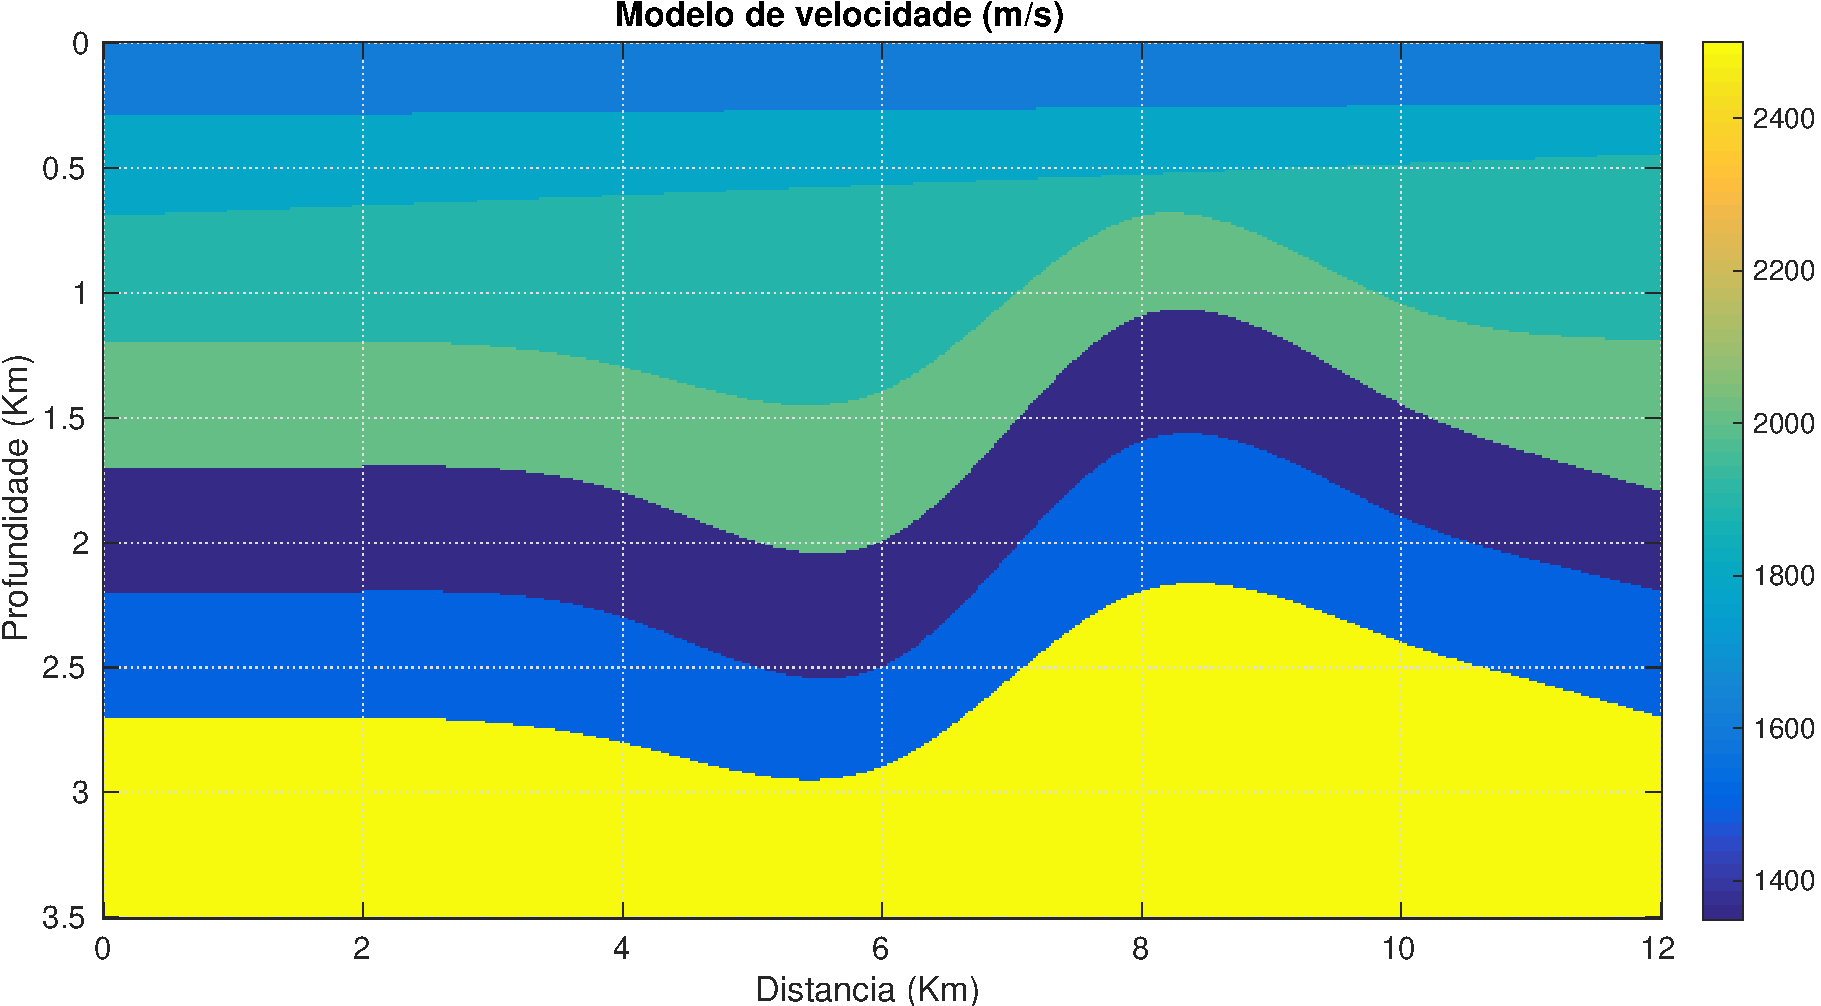
\includegraphics[totalheight=14cm]{figuras/cap2/modelo_de_velocidade.pdf}
\caption{Modelo 2D de velocidade das camadas referente a Figura \ref{fig:vagarosidade}.}
\label{fig:modelo_velocidade}
\end{figure}
\end{landscape}

A escolha de um fluxo de processamento a ser utilizado não é única para todo e qualquer experimento sísmico de reflexão. As etapas deste fluxo devem ser criteriosamente analisados de acordo com o objetivo desejado. Desta maneira, as etapas de um fluxo de processamento convencional são completamente diferentes das etapas de um processamento sísmico visando análise da variação da amplitude com o offset (AVO), por exemplo. Sendo assim, o fluxo a ser seguido dependerá da qualidade do dado adquirido em levantamento, das ferramentas, disponíveis (software e hardware), da experiência de quem processa o dado, do tempo disponível para o processamento das imagens e do objetivo que espera ser alcançado. \citep{Soares(2009)}

% \begin{figure}[H]
% \centering
% 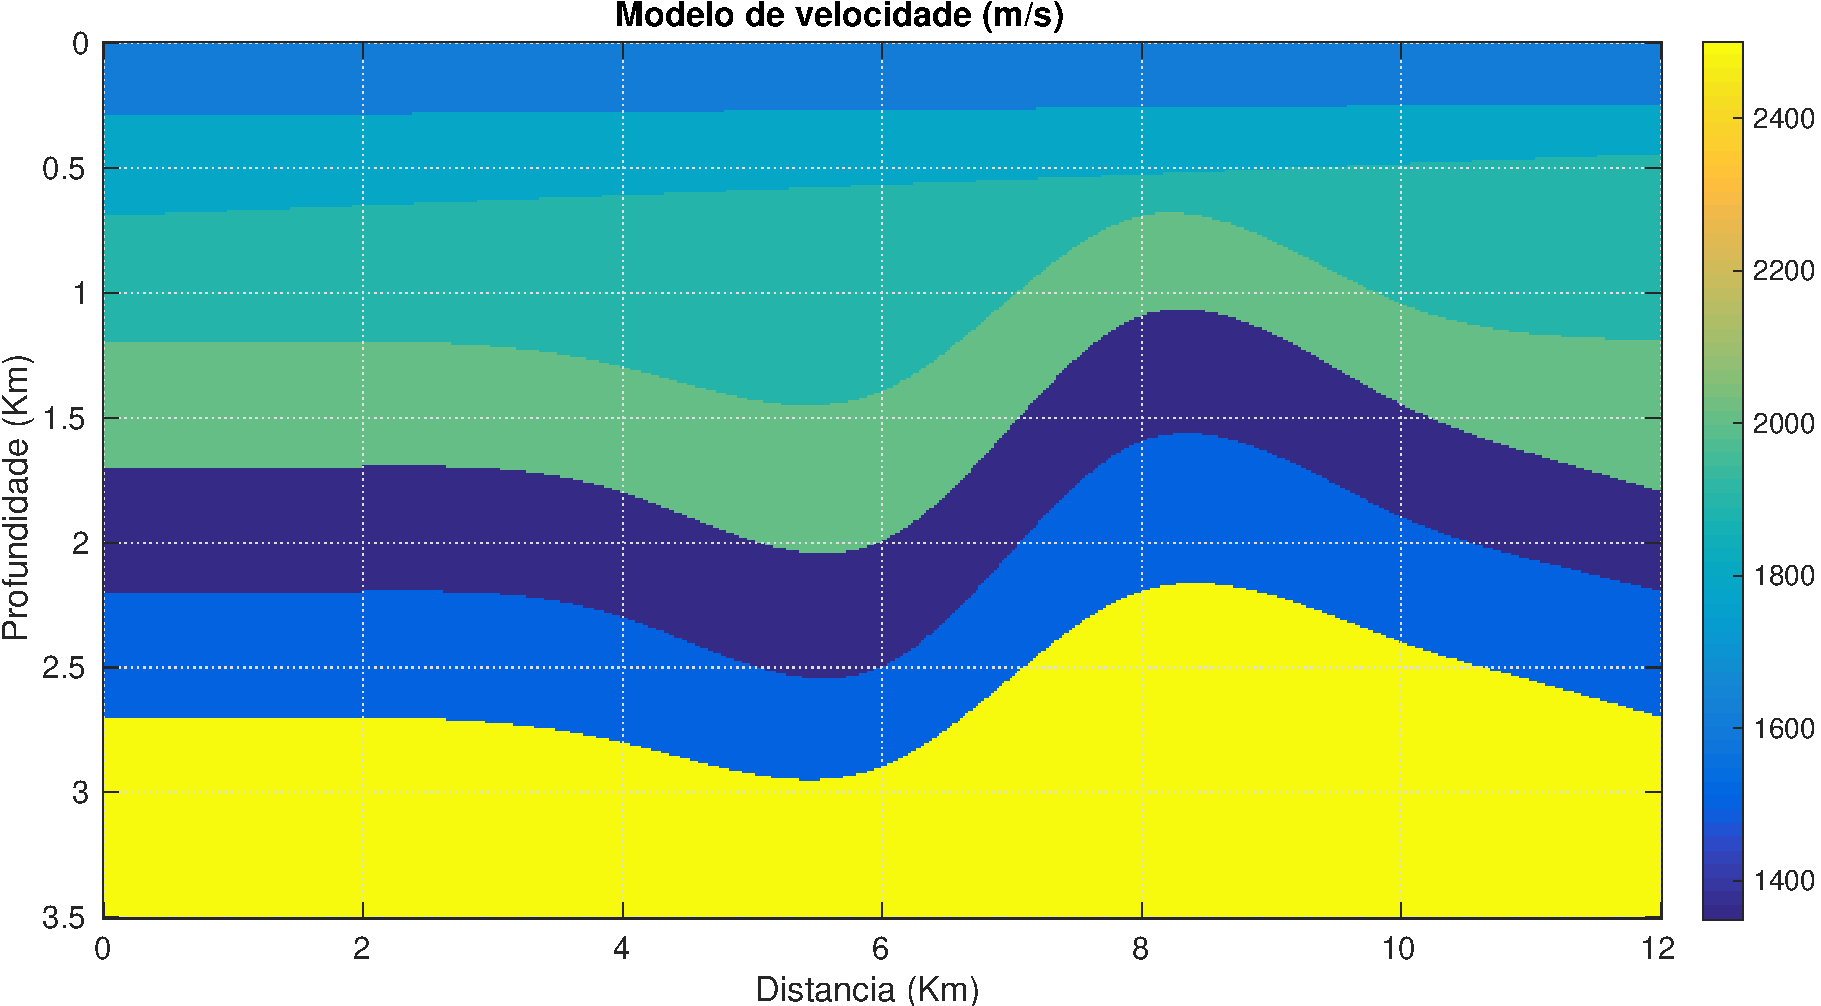
\includegraphics[totalheight=14cm]{figuras/cap2/modelo_de_velocidade.pdf}
% \caption{Modelo 2D de velocidade das camadas referente a figura \ref{fig:vagarosidade}.}
% \label{fig:modelo_velocidade}
% \end{figure}

\section{GEOMETRIA E PARÂMETROS DE AQUISIÇÃO}

O termo Geometria é utilizado para designar a fase do processamento na qual são inseridas as informações a respeito de localização de cada fonte (tiro) e cada receptor (arranjo de hidrofones ou geofones), através de suas coordenadas. Essas informações serão inseridas no header dos traços sísmicos, permitindo que todas as etapas posteriores possam ser realizadas.

\begin{figure}[H]
\centering
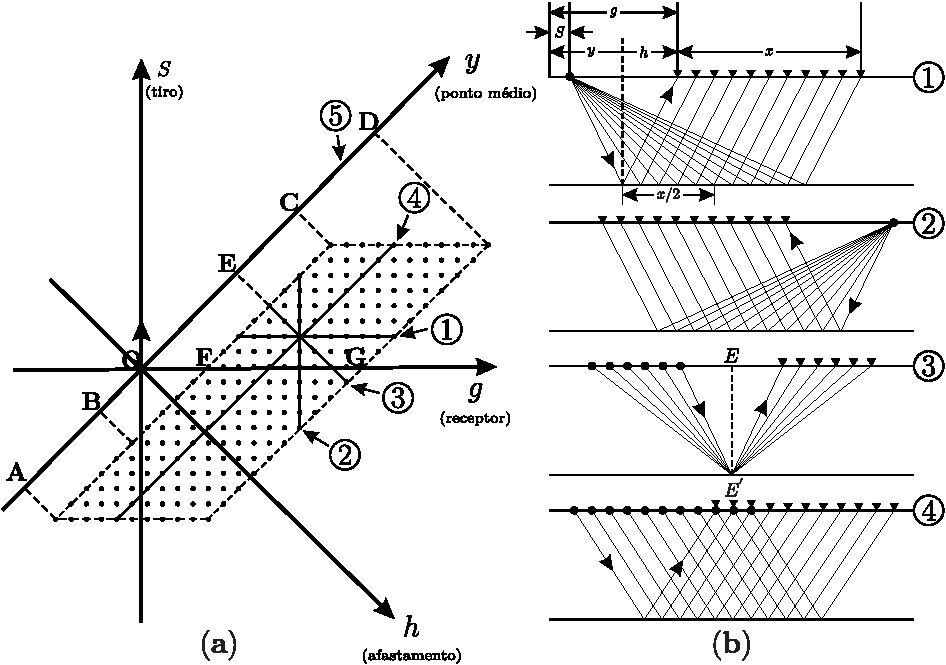
\includegraphics[width=12cm]{figuras/cap2/geometria.pdf}
\caption{Geometria de aquisição, para vários tiros com a orientação cartesiana para obter uma melhor visualização das famílias comuns. Um dado sísmico pode ser organizado em família de tiro comum (1); receptor comum (2); ponto médio comum (3); e (4) afastamento comum (offset comum). Figura adaptada de \citep{Yilmaz(2000)}}
\label{fig:geometria_cdp}
\end{figure}

Ponto comum em profundidade. Nome de uma técnica de levantamento de reflexão sísmica idealizada por W. Harry Mayne, em 1962, na qual os pontos de subsuperfície são registrados, redundantemente, com diferentes distâncias fonte-receptor. Esta técnica de aquisição trás a vantagem de se poder aumentar a razão sinal-ruído através da soma dos traços com o mesmo CMP, designada por \textit{stack}. Quando os traços com o mesmo CMP são agrupados formam um \textit{CMP gather}. 

Para se obter um sismograma sintético a partir de uma modelagem sísmica é preciso definir, inicialmente, a geometria de aquisição de dados e os seus parâmetros de aquisição. Neste sistema devem ser estabelecidas: a quantidade de receptores, a distância entre a fonte e o primeiro receptor e a distância entre os demais receptores, conforme a tabela \ref{tab:tab3}.

% \begin{table}[H]
% \centering
% \begin{tabular}{|l|c|}
% \hline
% \multicolumn{2}{|c|}{Parâmetros de aquisição do dado sintético} \\ \hline
% Distância entre geofones (m)               & 25                 \\ \hline
% Distância entre tiros (m)                  & 50                 \\ \hline
% Offset (m)                                 & -1175              \\ \hline
% Comprimento do lanço (m)                   &                    \\ \hline
% Número de tiros                            & 193                \\ \hline
% Número de amostras por traço               & 1200               \\ \hline
% Tempo de amostragem (ms)                   & 4000               \\ \hline
% \end{tabular}
% \caption{Parâmetros de aquisição do dado sintético.}
% \label{tab:tab2}
% \end{table}

As informações a respeito dos parâmetros de aquisição são importantes para todas as etapas de processamento do dado. Utilizamos o programa \textit{triseis} do \textit{Seismic Unix} (Anexo B) que tem por objetivo gerar os traços sísmicos referente a resposta do modelo de camadas curvas. O programa se basea na teoria de raios e gera os sismogramas sintéticos de feixes Gaussianos, a partir de um modelo triangularizado preenchido (triângulos) com os valores de vagarosidade. Os parâmetros requeridos pelo programa são:

\begin{itemize}
 \item xs: coordenadas da fonte
 \item zs: profundidade da fonte em superfície
 \item xg: coordenada dos receptores em superfície
 \item zg: profundidade dos receptores
\end{itemize}

A operação do programa funciona funciona dentro de três loops sucessivos. Isto ocorre de forma que o \textit{i-loop} referente às posições da fonte depende da conclusão do \textit{j-loop} que descreve cada posição de receptor, que por sua vez, depende de \textit{k-loop}, que mapeia cada refletor separadamente. Portanto, todos os raios referente ao primeiro refletor (localizados na interface 2), são armazenados nos receptores, para o primeiro tiro. Em seguida todos os raios varrem o segundo refletor (interface 3) e são armazenados em cada receptor novamente ainda para o primeiro tiro. Quando todos os refletores são mapeados é que ocorre o loop da posição da fonte varrendo a dimensão do modelo.

O arranjo utilizado ``split-spread'' simétrico figura \ref{fig:split_spread} possui o mesmo número de recpetores (geofones) equiespaçados linearmente em ambos os lados da coordenada de tiro. A distância entre a fonte e o primeiro receptor é conhecida como afastamento mínimo. A figura \ref{fig:afastamento_min} mostra o afastamento mínimo entre fonte e receptor.

\begin{figure}[H]
\centering
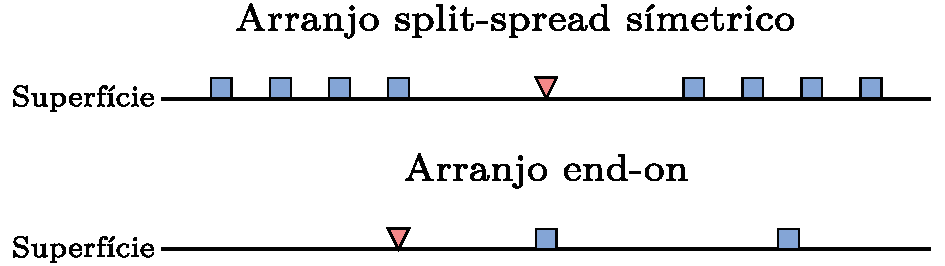
\includegraphics[height=2.5cm]{figuras/cap2/arranjo.pdf}
\caption{Arranjo split spread simétrico e end-on, o arranjo split spread em relação a posição da fonte fornece cobertura simétrica sobre a fonte. Em vermelho a representação da fonte e em azul os recepetores (geofones).}
\label{fig:split_spread}
\end{figure}

Após a aquisição do dado sísmico é necessário carregar e organizar a geometria de aquisição, o SU permite adicionar e/ou modificar o header pelo programa \textit{suchw} (ver Anexo). O suchw calcula valores de uma chave do header, segundo a equação (\ref{eq:suchw}), utilizando os valores de chaves pré-existentes (offset, cdp). Neste programa carregamos a chave \textit{CDP} e organizamos os CDP's.

\begin{equation}
key3=\frac{(a+b*key1+c*key2)}{d}
\label{eq:suchw} 
\end{equation}

\begin{table}[H]
\centering
\begin{tabular}{|c|l|l|}
\hline
\textbf{Chaves} & \multicolumn{1}{c|}{\textbf{Descrição}}                                   & \multicolumn{1}{c|}{\textbf{Valores}} \\ \hline
tracl           & \begin{tabular}[c]{@{}l@{}}Contagem sequêncial dos\\ traços.\end{tabular} & 1 18528 (1 - 18528)                   \\ \hline
tracf           & Número do receptor.                                                       & 1 96 (1 - 96)                         \\ \hline
fldr            & Número do tiro.                                                           & 1 193 (1 - 193)                       \\ \hline
sx              & Posição do tiro.                                                          & 0 9600 (0 - 9600)                     \\ \hline
gx              & Posição do receptor                                                       & -1175 10800 (-1175 - 10800)           \\ \hline
offset          & Afastamento fonte – receptor.                                             & -1175 1200 (-1175 - 1200)             \\ \hline
cdp             & Ponto comum em profundidade.                                              & 1 10788 (1 - 10788)                   \\ \hline
trid            & Identificação do tipo de traço sísmico.                                   & 1                                     \\ \hline
dt              & Intervalo de amostragem.                                                  & 4000                                  \\ \hline
ns              & Número de amostras.                                                       & 1200                                  \\ \hline
\end{tabular}
\caption{Principais chaves do header de um arquivo SU, de acordo com o programa surange. Estas informação são referentes ao arranjo split-spread.}
\label{tab:tab3}
\end{table}


\begin{table}[H]
\centering
\begin{tabular}{|c|l|l|}
\hline
\textbf{Chaves} & \multicolumn{1}{c|}{\textbf{Descrição}}                                   & \multicolumn{1}{c|}{\textbf{Valores}} \\ \hline
tracl           & \begin{tabular}[c]{@{}l@{}}Contagem sequêncial dos\\ traços.\end{tabular} & 1 18528 (1 - 18528)                   \\ \hline
tracf           & Número do receptor.                                                       & 1 96 (1 - 96)                         \\ \hline
fldr            & Número do tiro.                                                           & 1 193 (1 - 193)                       \\ \hline
sx              & Posição do tiro.                                                          & 0 9600 (0 - 9600)                     \\ \hline
gx              & Posição do receptor                                                       & 50 14400 (50 - 14400)                 \\ \hline
offset          & Afastamento fonte – receptor.                                             & 50 4800 (50 - 4800)                   \\ \hline
cdp             & Ponto comum em profundidade.                                              & 25 12000 (25 - 12000)                 \\ \hline
trid            & Identificação do tipo de traço sísmico.                                   & 1                                     \\ \hline
dt              & Intervalo de amostragem.                                                  & 4000                                  \\ \hline
ns              & Número de amostras.                                                       & 1200                                  \\ \hline
\end{tabular}
\caption{Principais chaves do header de um arquivo SU, de acordo com o programa surange. Estas informação são relativas ao arranjo end-on.}
\label{tab:tab4}
\end{table}

\begin{landscape}
\begin{figure}[H]
\centering
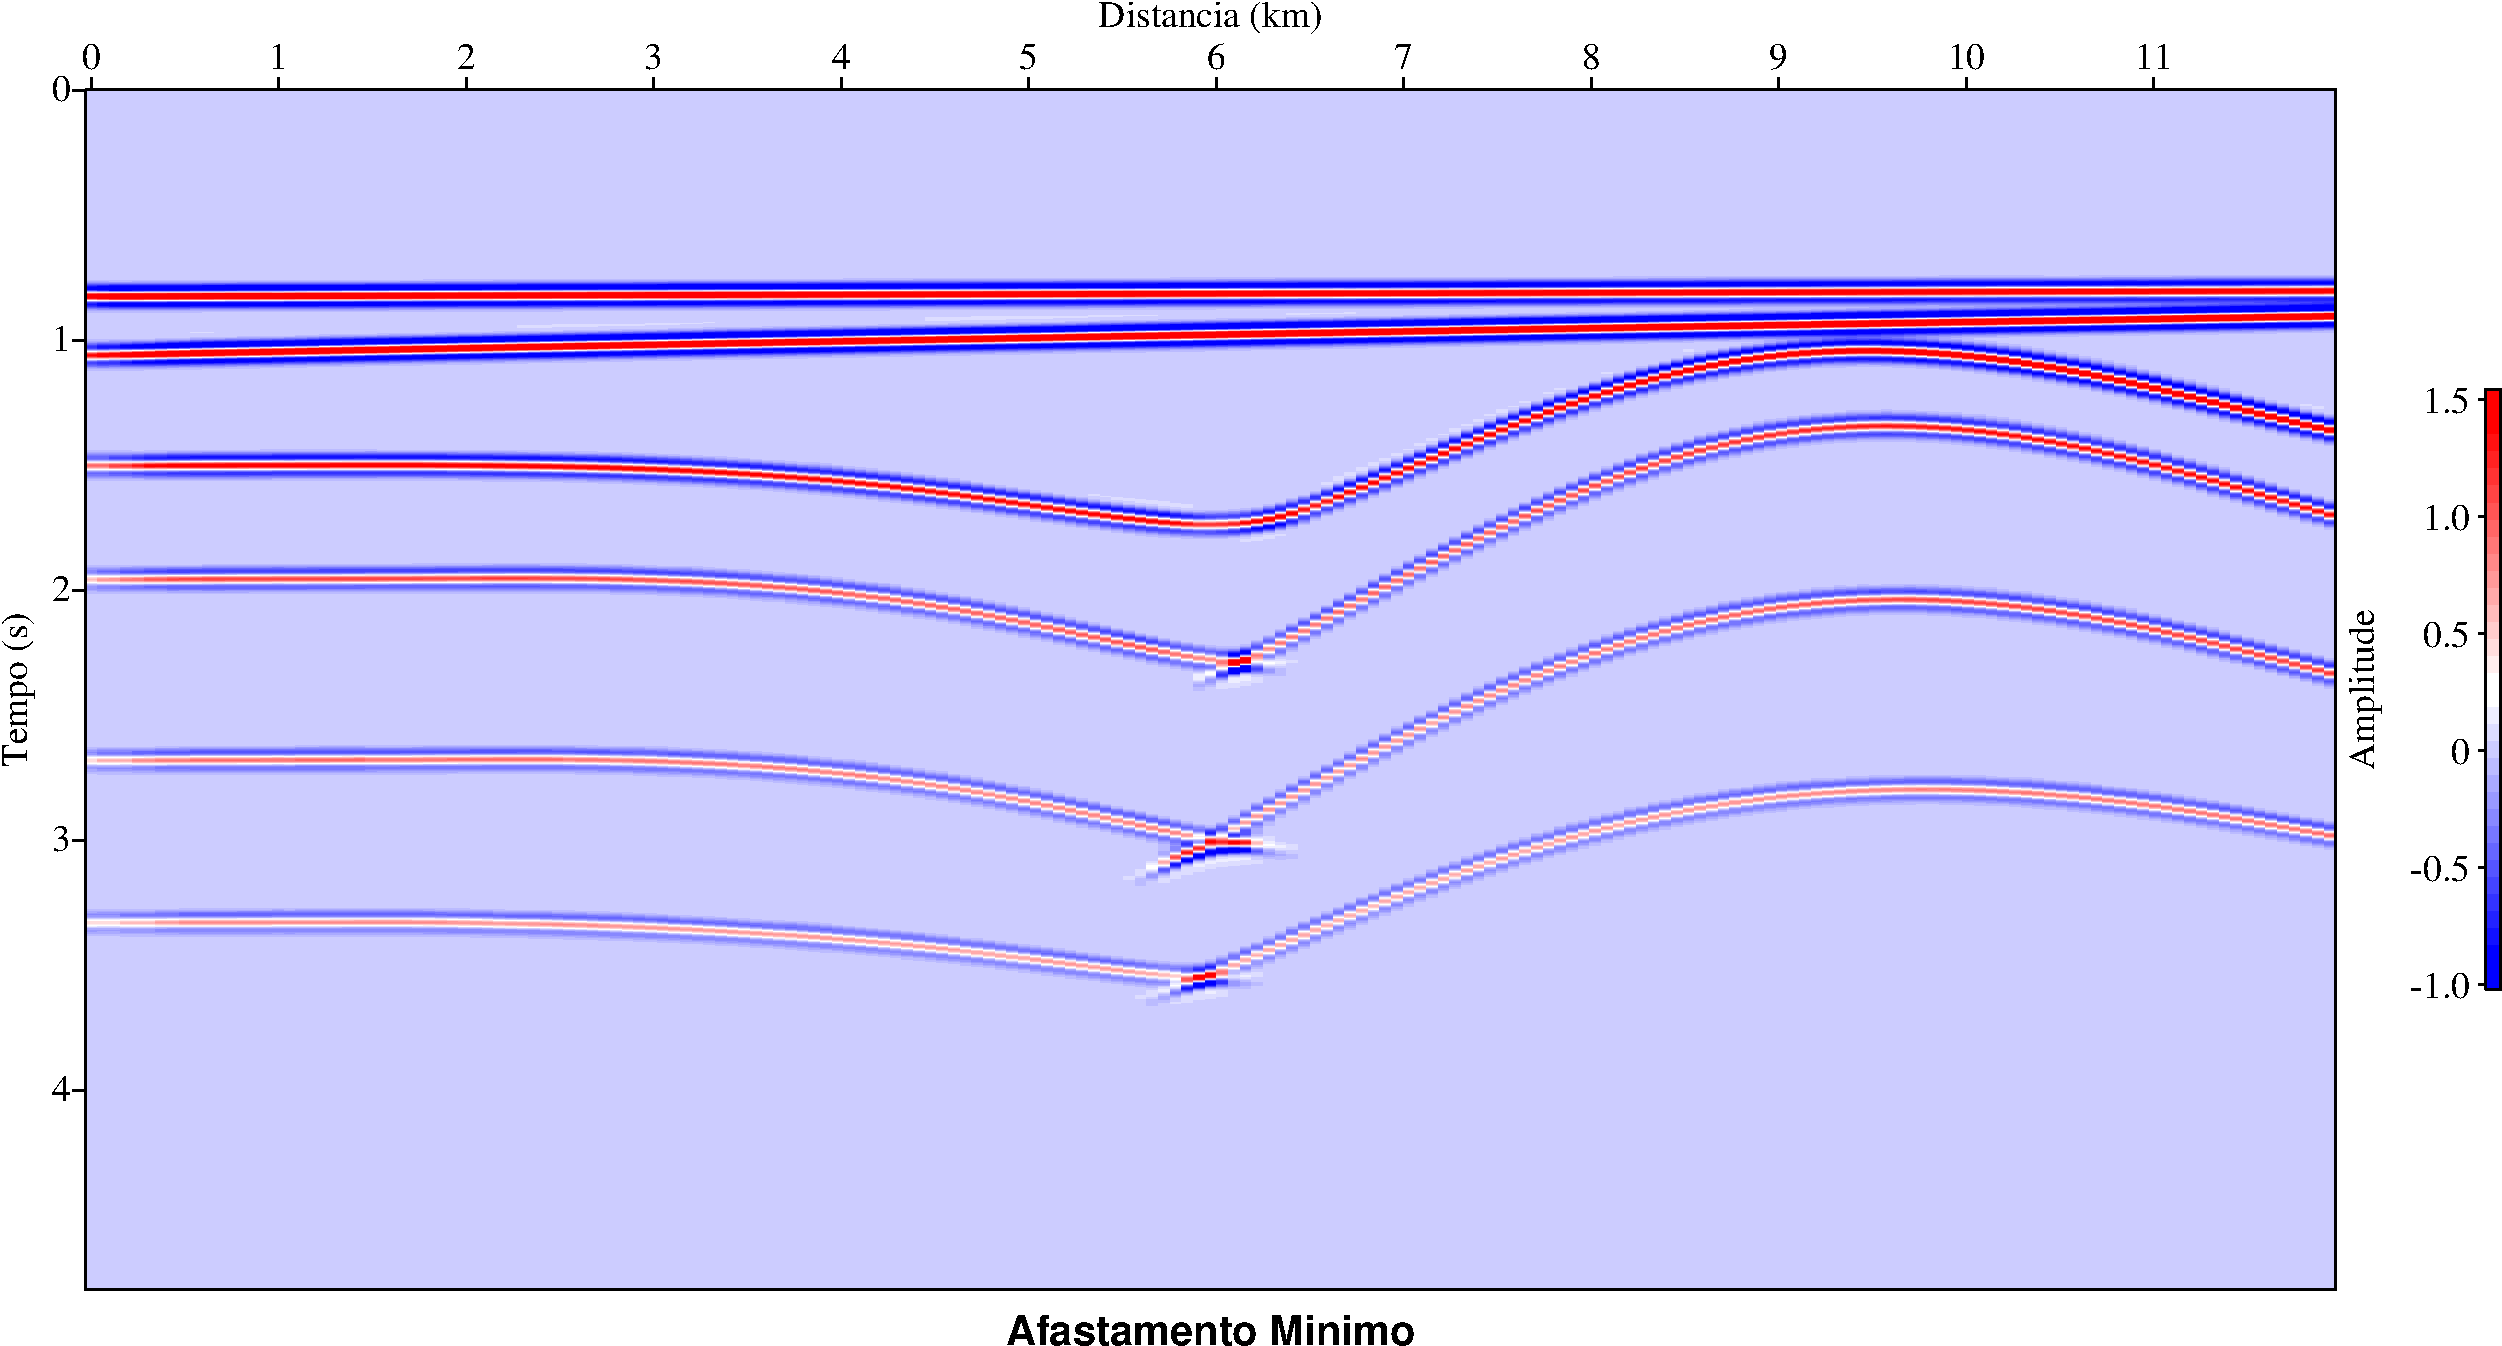
\includegraphics[totalheight=14cm]{figuras/cap2/seis_minoffset.pdf}
\caption{Afastamento mínimo entre fonte e receptor.}
\label{fig:afastamento_min}
\end{figure}
\end{landscape}

\section{TRANSFORMADA DE RADON LINEAR}

O nome da técnica (Radon) provém do matemático austríaco Johann Radon, responsável, em 1917, pela implementação dos fundamentos matemáticos para a reconstituição de imagens tomográficas. A transformada de Radon Linear (chamada também de tranformada $(\tau -p)$ ou ``Slant Stack - empilhamento oblíquo''): Consiste de uma soma ao longo de trajetórias (retas) aplicada ao dado sísmico. A metodologia utilizada nesse trabalho para realizar a transformada de Radon linear, está no domínio da frequência.

Agora examinamos os aspectos físicos da construção de uma família de pilha inclinada ``slant-stack gather''. Cada traço nesta família representa uma onda plana que se propaga em um determinado ângulo da vertical. Na realidade, quando uma fonte de dinamite explode, a energia se propaga em todos os ângulos (Figura \ref{fig:radon1}). A energia refletida chega a diferentes grupos de receptores em ângulos diferentes devido ao deslocamento entre os locais da fonte e do receptor. Quanto mais afastada ou mais rasa a interface refletora, mais oblíquo o ângulo da próxima frente de onda \citep{Yilmaz(2000)}.

\begin{figure}[H]
\centering
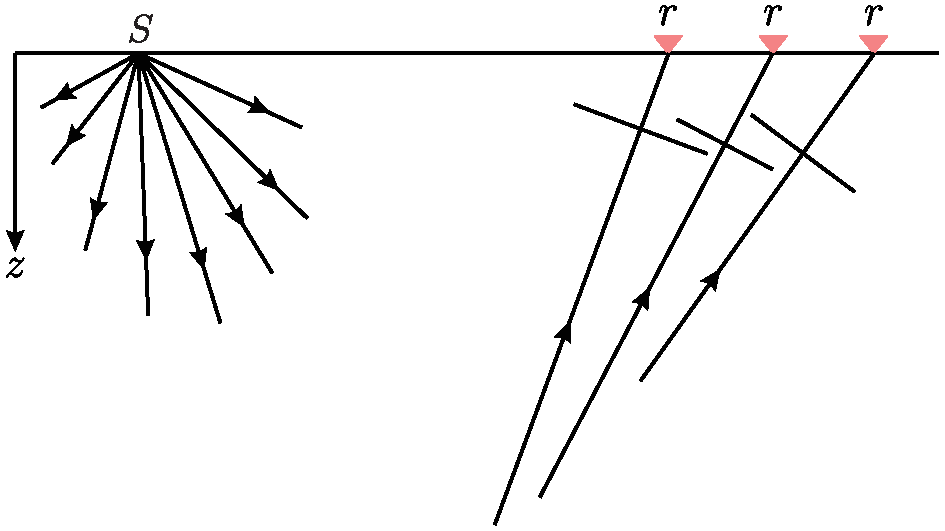
\includegraphics[width=11cm]{figuras/cap2/radon1.pdf}
\caption{Uma fonte sísmica gera ondas que se propagam em todas as direções, as ondas que se propagam em diferentes direções são registradas em diferentes locais do receptor.}
\label{fig:radon1}
\end{figure}

Como um auxílio na definição de um esquema para a construção da família de pilha inclinada, primeiro considere como as ondas planas podem ser geradas. Imagine uma linha de fontes pontuais, como mostra a Figura \ref{fig:radon2}. Suponha que essa linha de fontes seja ativada para que todos os pontos da linha sejam excitados simultaneamente e cada ponto gere um campo de ondas esférico.

\begin{figure}[H]
\centering
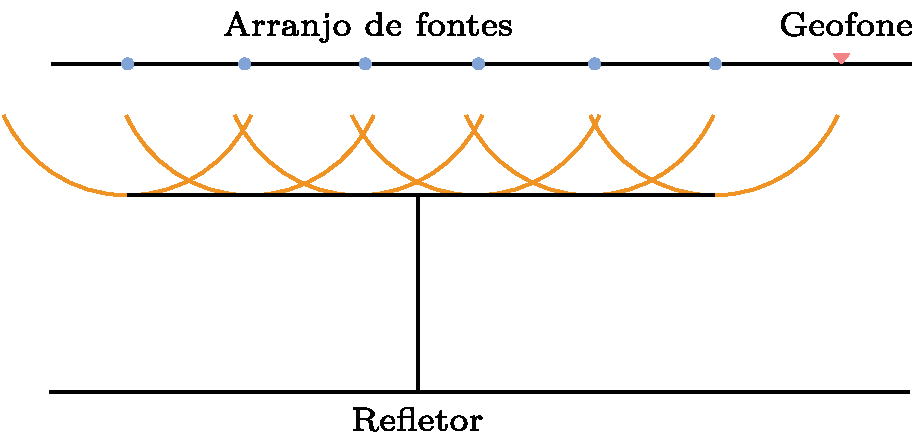
\includegraphics[width=11cm]{figuras/cap2/radon2.pdf}
\caption{Uma fonte sísmica gera ondas que se propagam em todas as direções, as ondas que se propagam em diferentes direções são registradas em diferentes locais do receptor.}
\label{fig:radon2}
\end{figure}

A alguma distância da superfície, as frentes de onda esféricas se sobrepõem e resultam em uma onda plana que viaja verticalmente para baixo. Essa onda plana reflete a partir de uma interface e é gravada por um receptor na superfície. (Na verdade, existem tipos de fontes, como Geoflex e Primacord, que aproximam as fontes de linhas curtas.)

Em vez de uma onda plana que se propaga verticalmente, uma onda plana que viaja no ângulo desejado a partir da vertical pode ser gerada usando a mesma linha de fontes pontuais, como ilustrado na Figura \ref{fig:radon3}. Para fazer isso, as fontes pontuais devem ser ativadas sucessivamente, começando em uma extremidade da linha com um atraso de tempo igual entre elas. Quando uma fonte pontual específica é ativada, a frente de onda gerada a partir da localização da fonte anterior já terá percorrido uma certa distância para a Terra. Quando todas as frentes de onda esféricas geradas pelas várias fontes se sobrepõem, o resultado é um plano inclinado em frente de onda. Essa onda plana se propaga, reflete a partir de uma interface e é gravada por um receptor na superfície.

\begin{figure}[H]
\centering
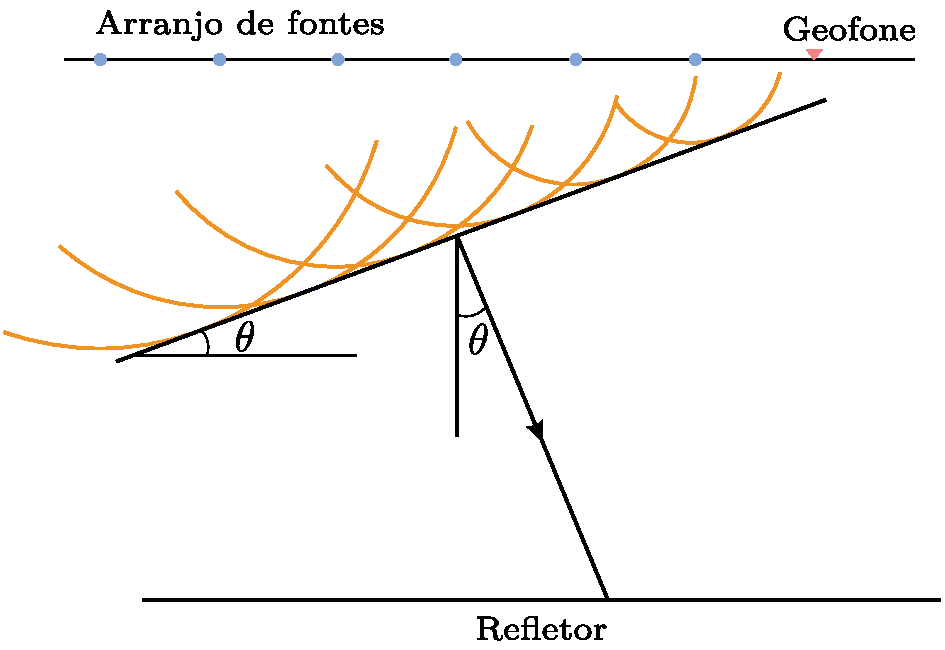
\includegraphics[width=10cm]{figuras/cap2/radon3.pdf}
\caption{Uma onda plana que se propaga no ângulo $\theta$ da vertical é gerada utilizando múltiplos disparos (começando da esquerda) em intervalos de tempo apropriados.}
\label{fig:radon3}
\end{figure}

A quantidade de inclinação da frente de onda, definida pelo ângulo de propagação da onda plana, pode ser controlada. Considere a geometria da frente de onda do caminho de raio na Figura \ref{fig:radon4}. No momento em que a frente de onda gerada no local de origem $S_1$ atinge o ponto $A$ na subsuperfície, a fonte de ponto no local $S_2$ deve ser excitada para que o ângulo desejado seja atingido. Defina a distância entre $S_1$ e $S_2$ como $\Delta x$ e a velocidade média com a qual as ondas viajam como $v$. Se levar algum tempo para a frente de onda ir de $S_1$ a $A$, usando o triângulo $S_1 A S_2$, o ângulo de inclinação $\theta$ da onda plana é dada por

\begin{figure}[H]
\centering
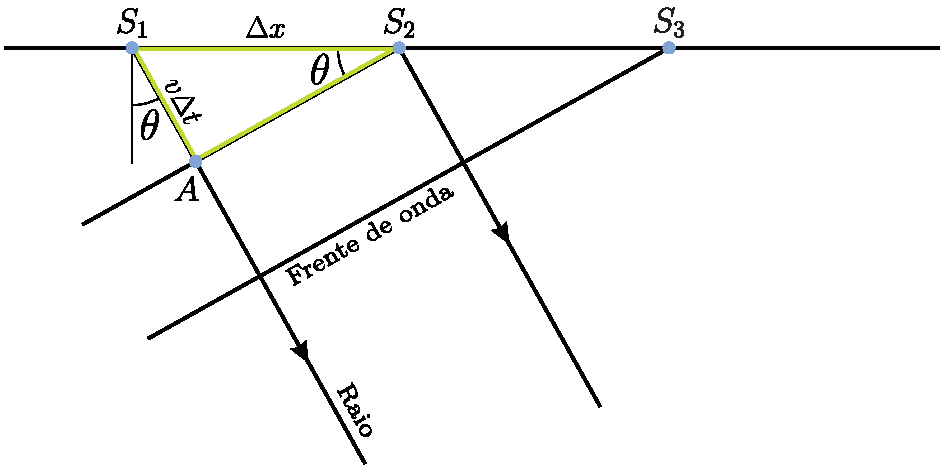
\includegraphics[width=12cm]{figuras/cap2/radon4.pdf}
\caption{Cálculo do intervalo de tempo entre os disparos ($S$) para gerar a onda plana oblíqua na Figura \ref{fig:radon3}.}
\label{fig:radon4}
\end{figure}

\begin{equation}
\sin \theta=\frac{v \Delta t}{\Delta x}.
\label{eq:6_1}
\end{equation}

O local da fonte ativa deve, portanto, viajar com a velocidade fornecida

\begin{equation}
\frac{\Delta x}{\Delta t}=\frac{v}{\sin \theta}
\label{eq:6_2}
\end{equation}

ao longo da direção horizontal, e a fonte do ponto na localização $S_2$ deve ser excitada para que possamos pegar a frente da onda em $S_1$ quando ela atingir o ponto $A$ na frente da onda na subsuperfície. A velocidade $(v/\sin\theta)$ com a qual a localização da fonte deve se mover é chamada \textit{velocidade de fase horizontal}.

A partir das experiências ilustradas nas Figuras \ref{fig:radon2} e \ref{fig:radon3}, observe que uma onda plana que se propaga em um ângulo da vertical pode ser gerada por:
\begin{enumerate}
 \item Colocando uma linha de fontes pontuais na superfície da Terra.
 \item Excitando as fontes pontuais em sucessão com um atraso de tempo.
 \item Sobrepondo as respostas que estão na forma de frentes de onda esféricas.
\end{enumerate}

A resposta sobreposta é gravada em um único receptor (Figura \ref{fig:radon3}). Essa resposta está na forma de uma onda plana que é refletida em uma interface. Superposição significa somar sobre o eixo do tiro para um determinado local do receptor. Usando o princípio da reciprocidade, a soma também pode ser realizada sobre o eixo do receptor para um determinado local do tiro.

Acabamos de discutir como uma família tiro comum com um único campo de ondas pode ser decomposta em seus componentes de ondas planas. Substituindo o eixo do tiro na Figura \ref{fig:radon4} pelo eixo receptor, a geometria do caminho do raio na Figura \ref{fig:radon5} resulta. O atraso de tempo associado à onda plana que viaja no ângulo $\theta$ na vertical e é dado por

\begin{equation}
\Delta t=\frac{\sin \theta}{v} \Delta x
\label{eq:6_3}
\end{equation}

\begin{figure}[H]
\centering
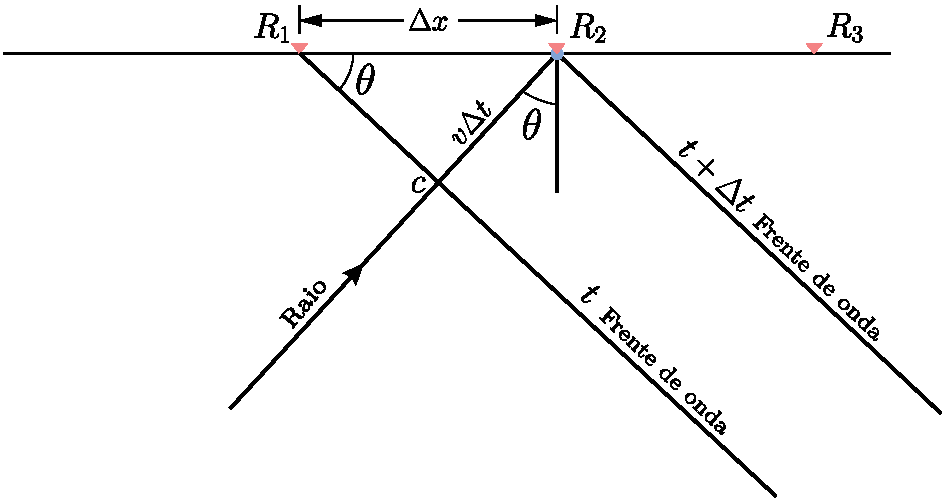
\includegraphics[width=12cm]{figuras/cap2/radon5.pdf}
\caption{O princípio da reciprocidade aplicado à geometria da Figura \ref{fig:radon4} para substituir os disparos ($S$) pelos receptores ($R$).}
\label{fig:radon5}
\end{figure}

A lei de Snell diz que a quantidade $\sin\theta/v$, que é o inverso da velocidade da fase horizontal, é constante

A lei de Snell diz que a quantidade $\sin\theta/v$, que é o inverso da velocidade da fase horizontal, é constante ao longo de um caminho de raio em um meio em camadas (Figura \ref{fig:radon6}). Essa constante é chamada de parâmetro de raio $p$. A equação (\ref{eq:6_3}) é reescrita como 

\begin{equation}
\sin\theta=\frac{v\Delta t}{\Delta x}
\label{eq:6_3b}
\end{equation}

\begin{figure}[H]
\centering
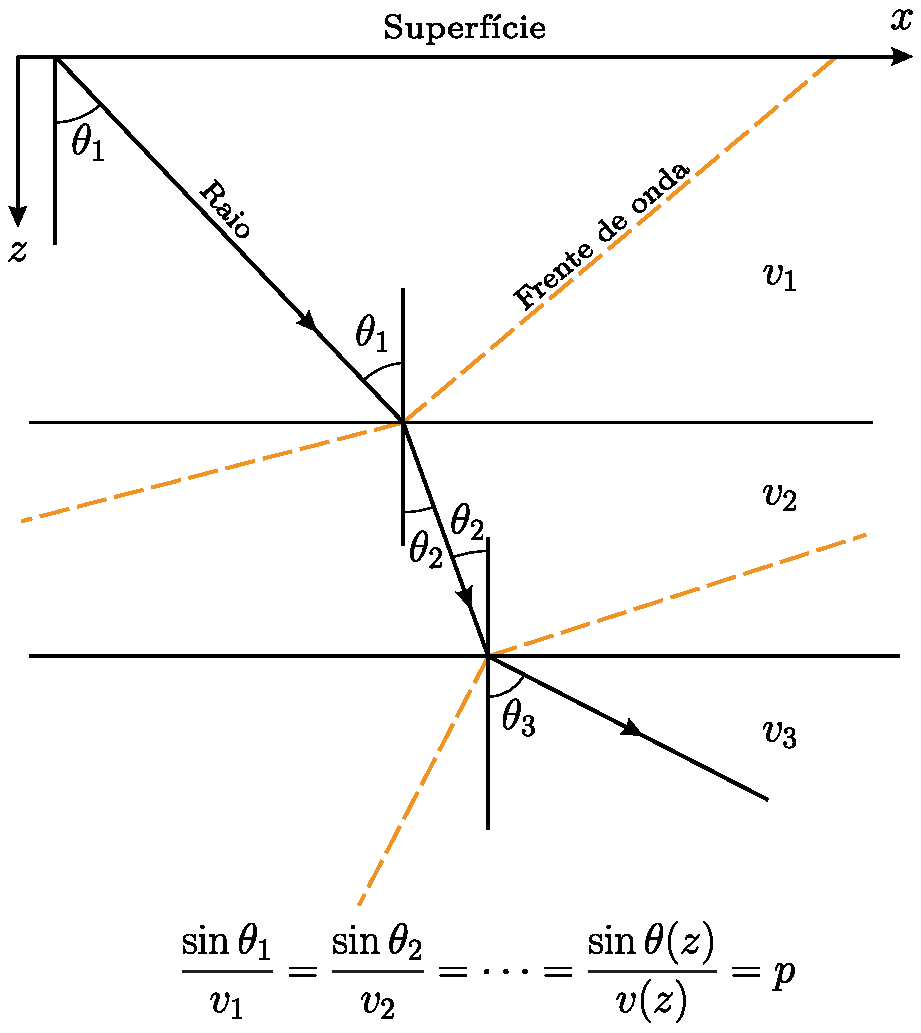
\includegraphics[width=9cm]{figuras/cap2/radon6.pdf}
\caption{Se o parâmetro de raio $p$ for especificado, o raio poderá ser traçado em um modelo de camadas horizontalmente com uma função de velocidade conhecida $v(z)$.}
\label{fig:radon6}
\end{figure}

O ângulo de propagação da onda plana é controlado ajustando o valor de $p$. Se o parâmetro de raio p for especificado, o raio poderá ser traçado em um modelo de camadas horizontalmente com uma função de velocidade conhecida $v(z)$. Definindo $p = 0$ corresponde a uma onda plana que se propaga verticalmente.
Dado o parâmetro de raio $p$ e a função de velocidade $v(z)$ para o modelo de camadas, a família de caminhos de raios associados a um valor de $p$ específico pode ser rastreada conforme mostrado na Figura 6.3-7. Uma onda plana que viaja em uma terra em camadas é chamada de onda Snell \citep{Claerbout(1978)}. Esse tipo de onda plana muda sua direção de propagação nos limites de cada camada, de acordo com a lei de Snell (Figura \ref{fig:radon6}). Para um único valor $p$, observe que o sinal é gravado com muitas compensações (offsets) (Figura \ref{fig:radon7}).

\begin{figure}[H]
\centering
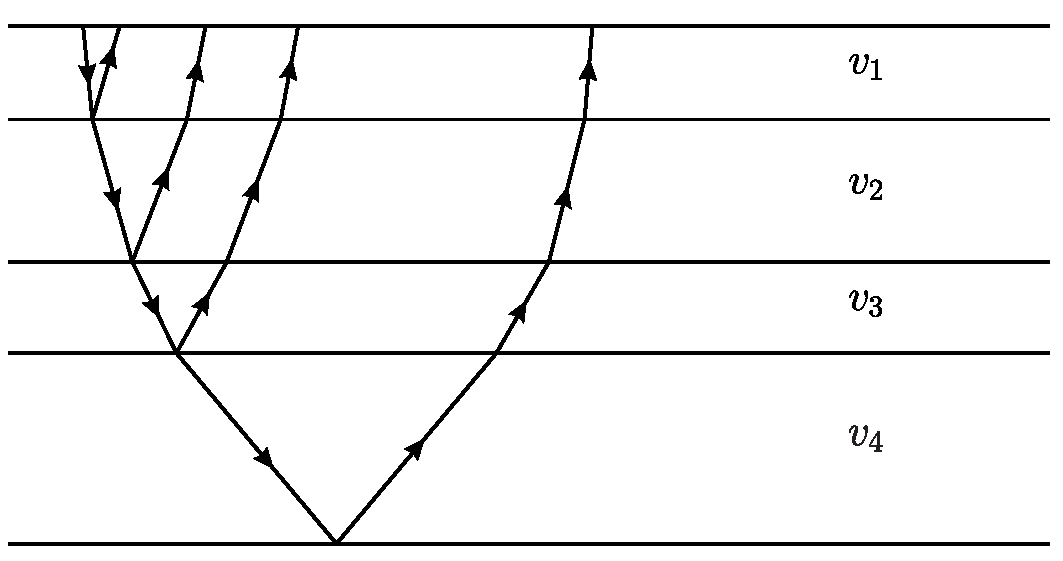
\includegraphics[width=10cm]{figuras/cap2/radon7.pdf}
\caption{Alguns caminhos de raio para um dado valor $p$, correspondendo a um único rastreamento (traço) no domínio $\tau - p$.}
\label{fig:radon7}
\end{figure}


Em geral, os receptores de todas os afastamentos registram ondas planas de muitos valores de $p$. Para decompor uma captura de tiro em seus componentes de onda plana, todas as amplitudes de traço na coleta devem ser somadas ao longo de vários caminhos inclinados, cada um com um atraso de tempo único definido pela equação (\ref{eq:6_3b}).

Enquanto não houver mergulho, os tempos de propagação em um tiro comum e em um ponto médio comum são indistinguíveis. Como um agrupamento CMP não é um campo de onda único, a decomposição de ondas planas parece não se aplicar aos agrupamentos de CMP. No entanto, a equivalência de um agrupamento CMP e  um agrupamento de tiros comuns em um modelo de camadas horizontais fornece uma justificativa para aplicar a decomposição de ondas planas nos dois tipos de agrupamentos (gathers).


\textbf{TRANSFORMADA SLANT-STACK}


Normalmente, duas etapas são usadas na síntese de ondas planas somando amplitudes no domínio de deslocamento ao longo de caminhos inclinados (Figura \ref{fig:radon8}). Primeiro, uma correção de movimento linear (LMO) é aplicada aos dados por meio de uma transformação de coordenadas definida por \citep{Claerbout(1978)}

\begin{equation}
\tau=t-p x,
\label{eq:6_4a}
\end{equation}

onde $p$ é o parâmetro de raio, $x$ é o deslocamento, $t$ é o tempo de viagem duplo e $\tau$ é o tempo de interceptação em $p = 0$. Em seguida, os dados são somados sobre o eixo de deslocamento (offset) por
\begin{equation}
S(p, \tau)=\sum_{x} P(x, \tau+p x),
\label{eq:6_4b}
\end{equation}

onde $S(p, \tau)$ representa uma onda plana com parâmetro de raio $p = sin\theta/v$. Repetindo a correção LMO para uma faixa de valores de $p$ e realizando a soma na equação (\ref{eq:6_4b}), é construída uma coleta de pilha inclinada completa. Uma pilha inclinada reúne, na prática, alternativamente é referido como uma coleta $\tau - p$; consiste em todos os componentes de mergulho dentro da faixa especificada de valores de $p$ nos dados de deslocamento originais.

O mapeamento do domínio $t - x$ para o domínio $\tau - p$ é reversível \citep{Thorson(1978)}. Primeiro, aplique a correção de movimento linear inverso (LMO) aos dados no domínio $\tau - p$
\begin{equation}
t=\tau+p x.
\label{eq:6_5a}
\end{equation}

Em seguida, some os dados no domínio $\tau - p$ sobre o parâmetro de raio eixo $p$ para obter
\begin{equation}
P(x, t)=\sum_{p} S(p, t-p x).
\label{eq:6_5b}
\end{equation}


\begin{figure}[H]
\centering
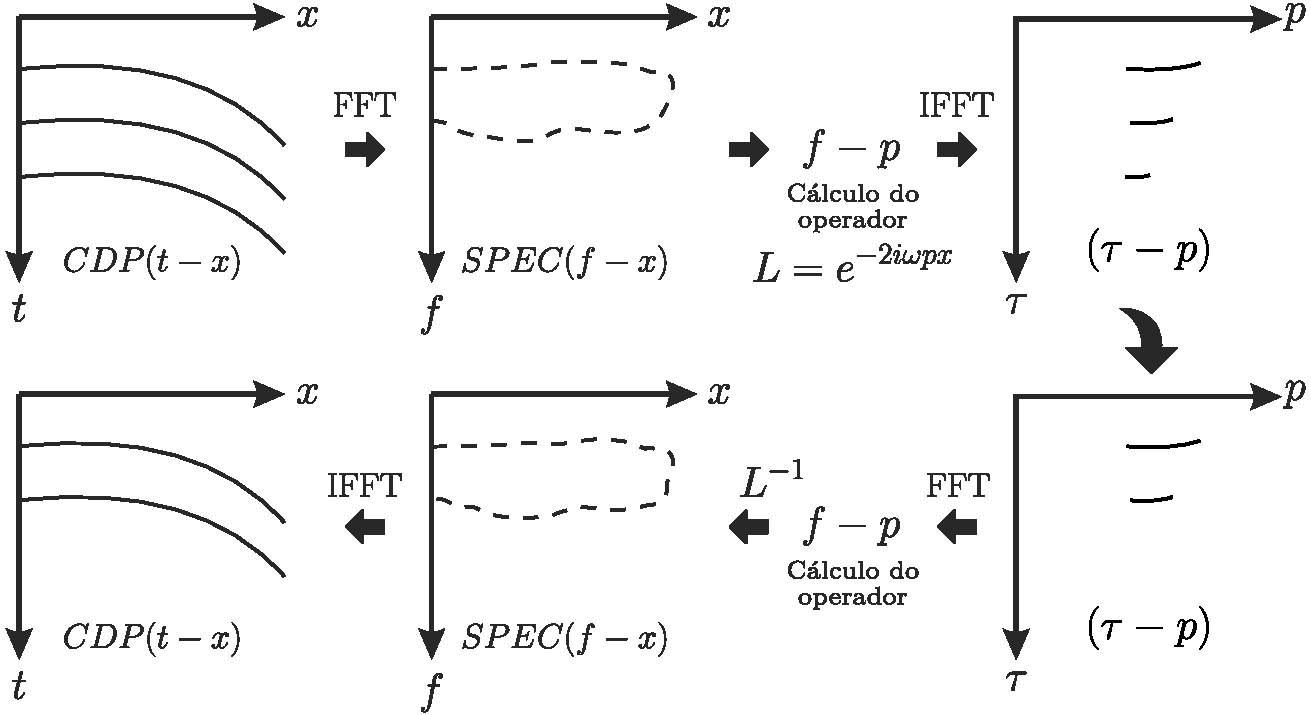
\includegraphics[width=15cm]{figuras/cap2/radon8.pdf}
\caption{Etapas para a construção do empilhamento oblíquo.}
\label{fig:radon8}
\end{figure}

%--------------------------------------------------------------------------------------------------------
\begin{landscape}
\begin{figure}[H]
\centering
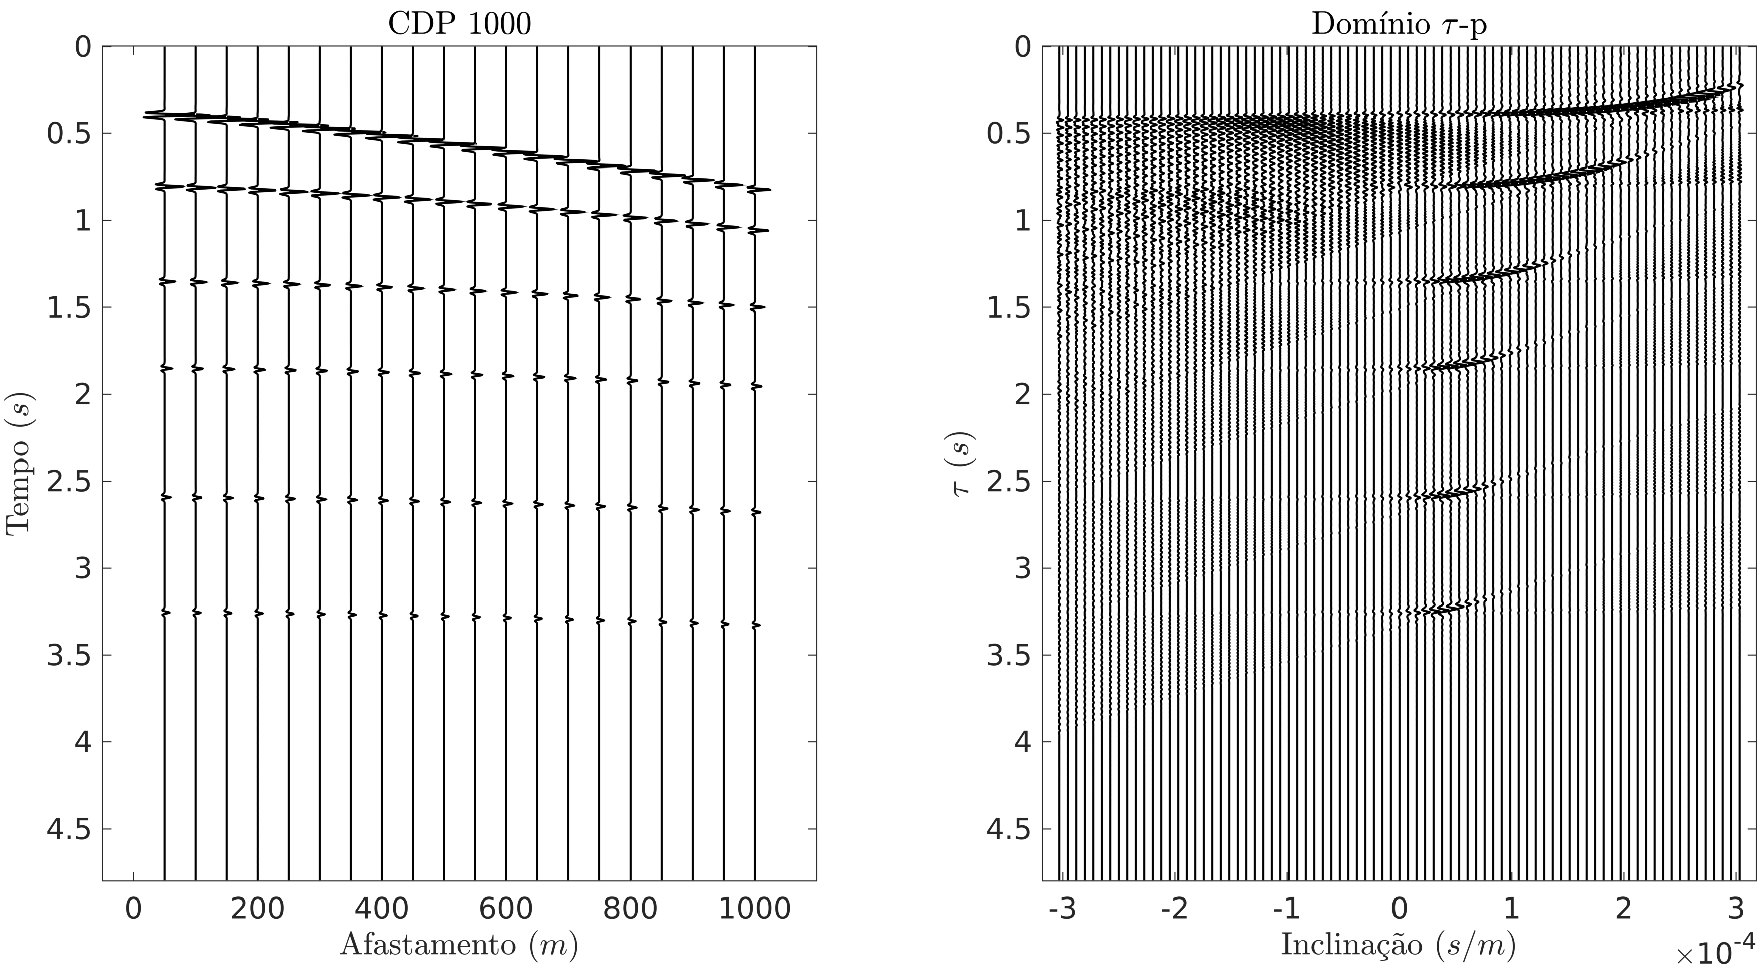
\includegraphics[totalheight=14cm]{figuras/cap2/radon_ida.pdf}
\caption{Transformada de Radon Linear direta do CDP-1000. (a) CDP-1000 no domínio $(x, t)$ e (b) CDP-1000 no domínio $(\tau, p)$.}
\label{fig:radon_ida}
\end{figure}
\end{landscape}
%-------------------------------------------------------------------------------------------------------
\begin{landscape}
\begin{figure}[H]
\centering
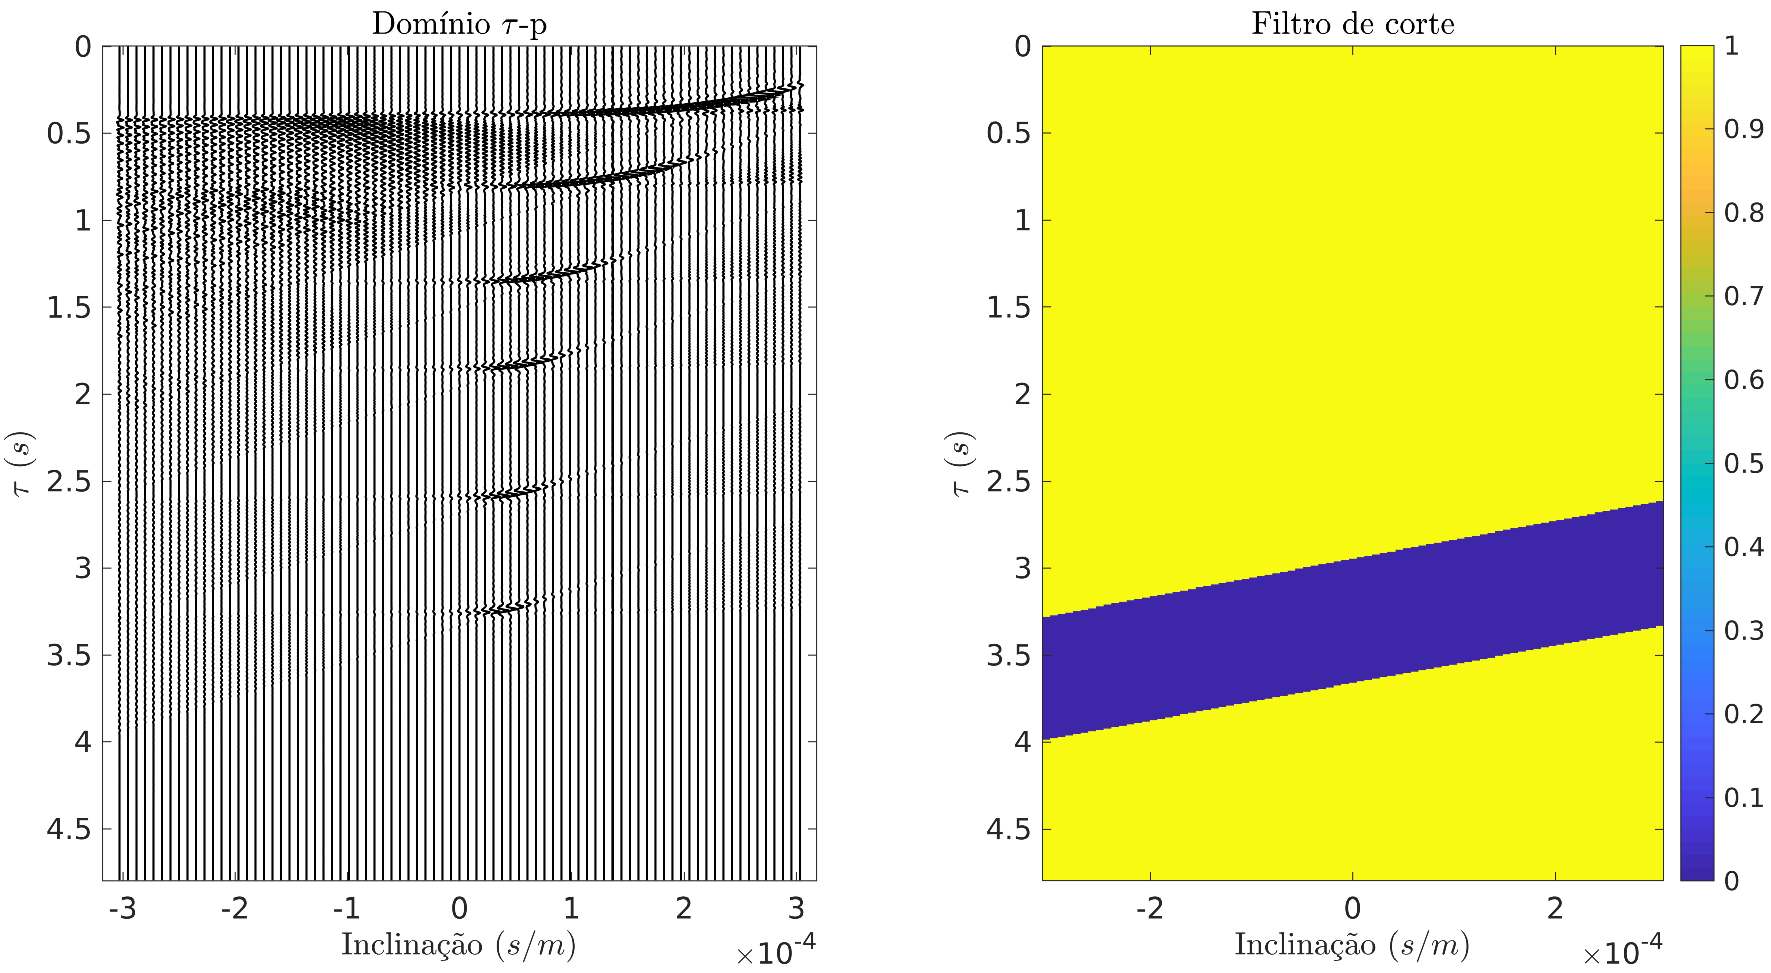
\includegraphics[totalheight=14cm]{figuras/cap2/Cut_off_Filter.pdf}
\caption{Transformada de Radon Linear direta do CDP-1000. (a) CDP-1000 no domínio $(\tau, p)$. (b) Filtro de corte aplicado no CDP-1000.}
\label{fig:filtro_radon}
\end{figure}
\end{landscape}
%-------------------------------------------------------------------------------------------------------
\begin{landscape}
\begin{figure}[H]
\centering
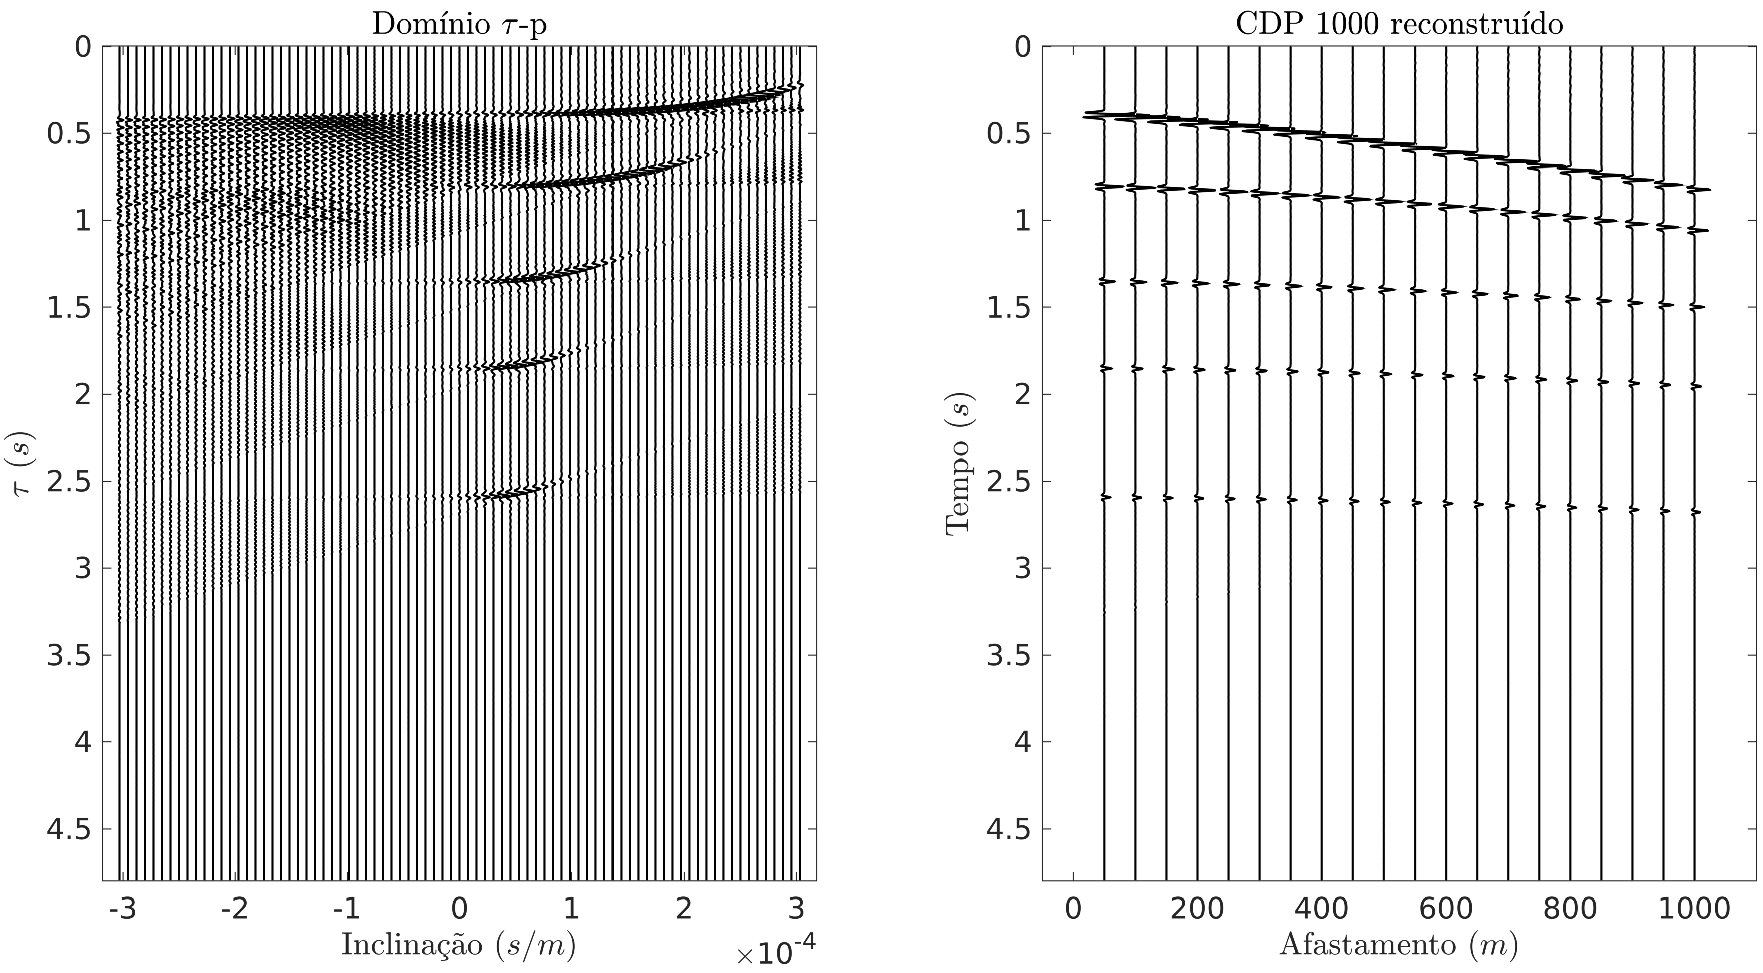
\includegraphics[totalheight=14cm]{figuras/cap2/radon_volta.pdf}
\caption{Transformada de Radon Linear inversa do CDP-1000. (a) CDP-1000 no domínio $(\tau, p)$ e (b) Reconstrução do CDP-1000 no domínio $(x, t)$ }
\label{fig:radon_volta}
\end{figure}
\end{landscape}

\section{TRANSFORMADA F-K}

A transformada de Fourier (TF) constitui um dos maiores produtos da física e da matemática, e é indispensável na teoria e no processamento de sinais por várias razões. 
Uma das primeiras é que a sua base é estruturada no conceito de \textit{frequência}, o que permite uma compreensão melhor do fenômeno sendo estudado, e que adiciona um complemento ao sinal temporal (espacial) que é inicialmente usado para análise. 
Esta condição é muito comum, e os exemplos são vários na física de ondas (como na acústica, sísmica, eletromagnetismo, vibrações, ótica, etc.), bem como em outras áreas onde processos periódicos são importantes e regem os fenômenos de interesse (como na biomedicina, biologia, astronomia, economia, etc.). \citep{Lourenildo(2015)}

Para tornar a descrição mais prática, define-se o par das integrais direta, $G(\omega)$, e inversa, $g(t)$, em 1D nas seguintes formas ilimitadas (o que se faz para um lado $t,\omega \rightarrow +\infty$ se faz para o outro $t,\omega \rightarrow -\infty$):
\begin{equation}
G(\omega)=k_{1}\int_{-\infty}^{\infty}g(t)e^{-i\omega t}dt, \quad G(\omega)=F\{g(t)\}, \quad (i=\sqrt{-1}),
\label{eq.3.1}
\end{equation}
\begin{equation}
g(t)=k_{2}\int_{-\infty}^{\infty}G(\omega)e^{+i\omega t}d\omega, \quad g(t)=F^{-1}\{G(\omega)\}, \quad (\omega=2\pi f).
\label{eq.3.2}
\end{equation}
A escolha dos coeficientes $k_{1}$ e $k_{2}$ dependem do usuário ou do problema em estudo. O requerimento é que o produto $k_{1}k_{2}=1/2\pi$. Se $k_{1}=k_{2}$, então, $k_{1}=1/\sqrt{2\pi}$. Se $k_{1}=1$, então, $k_{2}=1/2\pi$.

Para o caso 2D, temos a TF direta na forma da equação (\ref{eq.3.3}) e TF inversa na equação (\ref{eq.3.4})

\begin{equation}
h(t, x)=\int_{-\infty}^{\infty} \int_{-\infty}^{\infty} H(f_{t}, f_{x}) e^{+i 2 \pi(f_{t} t+f_{x} x)} df_{t} df_{x}
\label{eq.3.3}
\end{equation}
\begin{equation}
H(f_{t}, f_{x})=\int_{-\infty}^{\infty} \int_{-\infty}^{\infty} h(t, x) e^{-i 2 \pi(f_{t} t+f_{x} x)} dt dx
\label{eq.3.4}
\end{equation}

Para estas equações se tem as relações: $f_{t}=\frac{1}{T} $, $f_{x}=\frac{1}{\lambda}=\frac{1}{vT}$, de onde se estabelece a relação $f_{t}=vf_{x}$; isto é, nestas condições a frequência temporal, $f_{t}$, e a frequência espacial, $f_{x}$, são acopladas através de uma relação linear $f_{t}=vf_{x}$, onde $v$ é o parâmetro de inclinação.
Também, usando a vagarosidade $s=\frac{1}{v}$ se tem a forma $f_{x}=sf_{t}$. 
A figura \ref{fig:Relacao_Dispersao} mostra a relação entre estas quantidades, com a descrição da propagação de uma onda plana, e a relação denominada de dispersão que envolve as frequências espaciais e a temporal.

\begin{figure}[H]
\centering
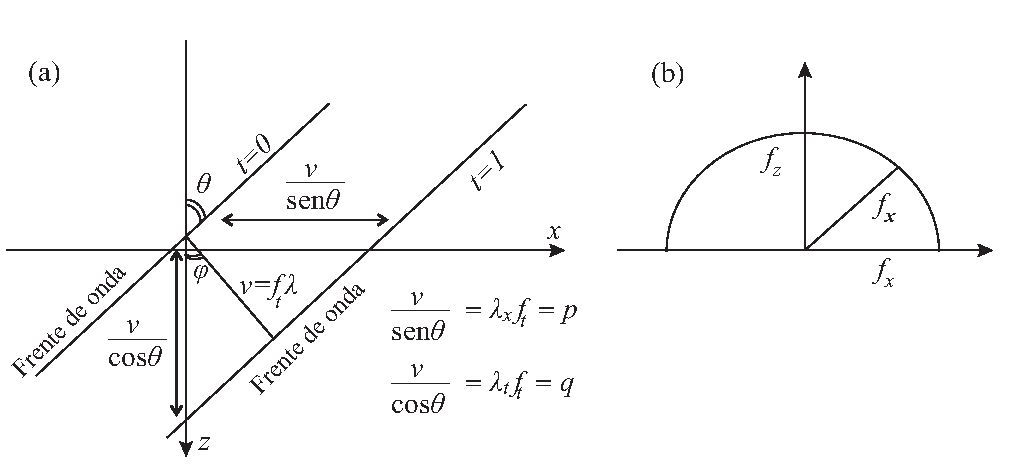
\includegraphics[width=12cm]{figuras/cap2/Relacao_Dispersao.pdf}
\vspace{-0.3cm}
\caption{Descrição física da relação entre a frente de onda e a equação da dispersão. 
(a) Propagação da onda plana. 
(b) Relação entre as componentes $f_{x}$ e $f_{z}$ e a total $f_{\mathbf{x}}$ para $f_{t}$ constante.}
\label{fig:Relacao_Dispersao}
\end{figure}

\section{FILTROS DE CORTE NA FREQUÊNCIA}

O princípio a ser aplicado é o de que os eventos possam ser separados no domínio da frequência, $f_{t}-f_{\mathbf{x}}$, de alguma forma, pelo menos parcial.  
Partindo deste princípio, a figura \ref{fig:Analise_Idealizada_Sinal_Ruido_Frequencia} ilustra a composição espectral, e serve para a análise da relação frequência temporal-espacial (número de onda) do conteúdo de velocidades comumente presente em experimentos de sísmica de exploração.

\begin{figure}[H]
\centering
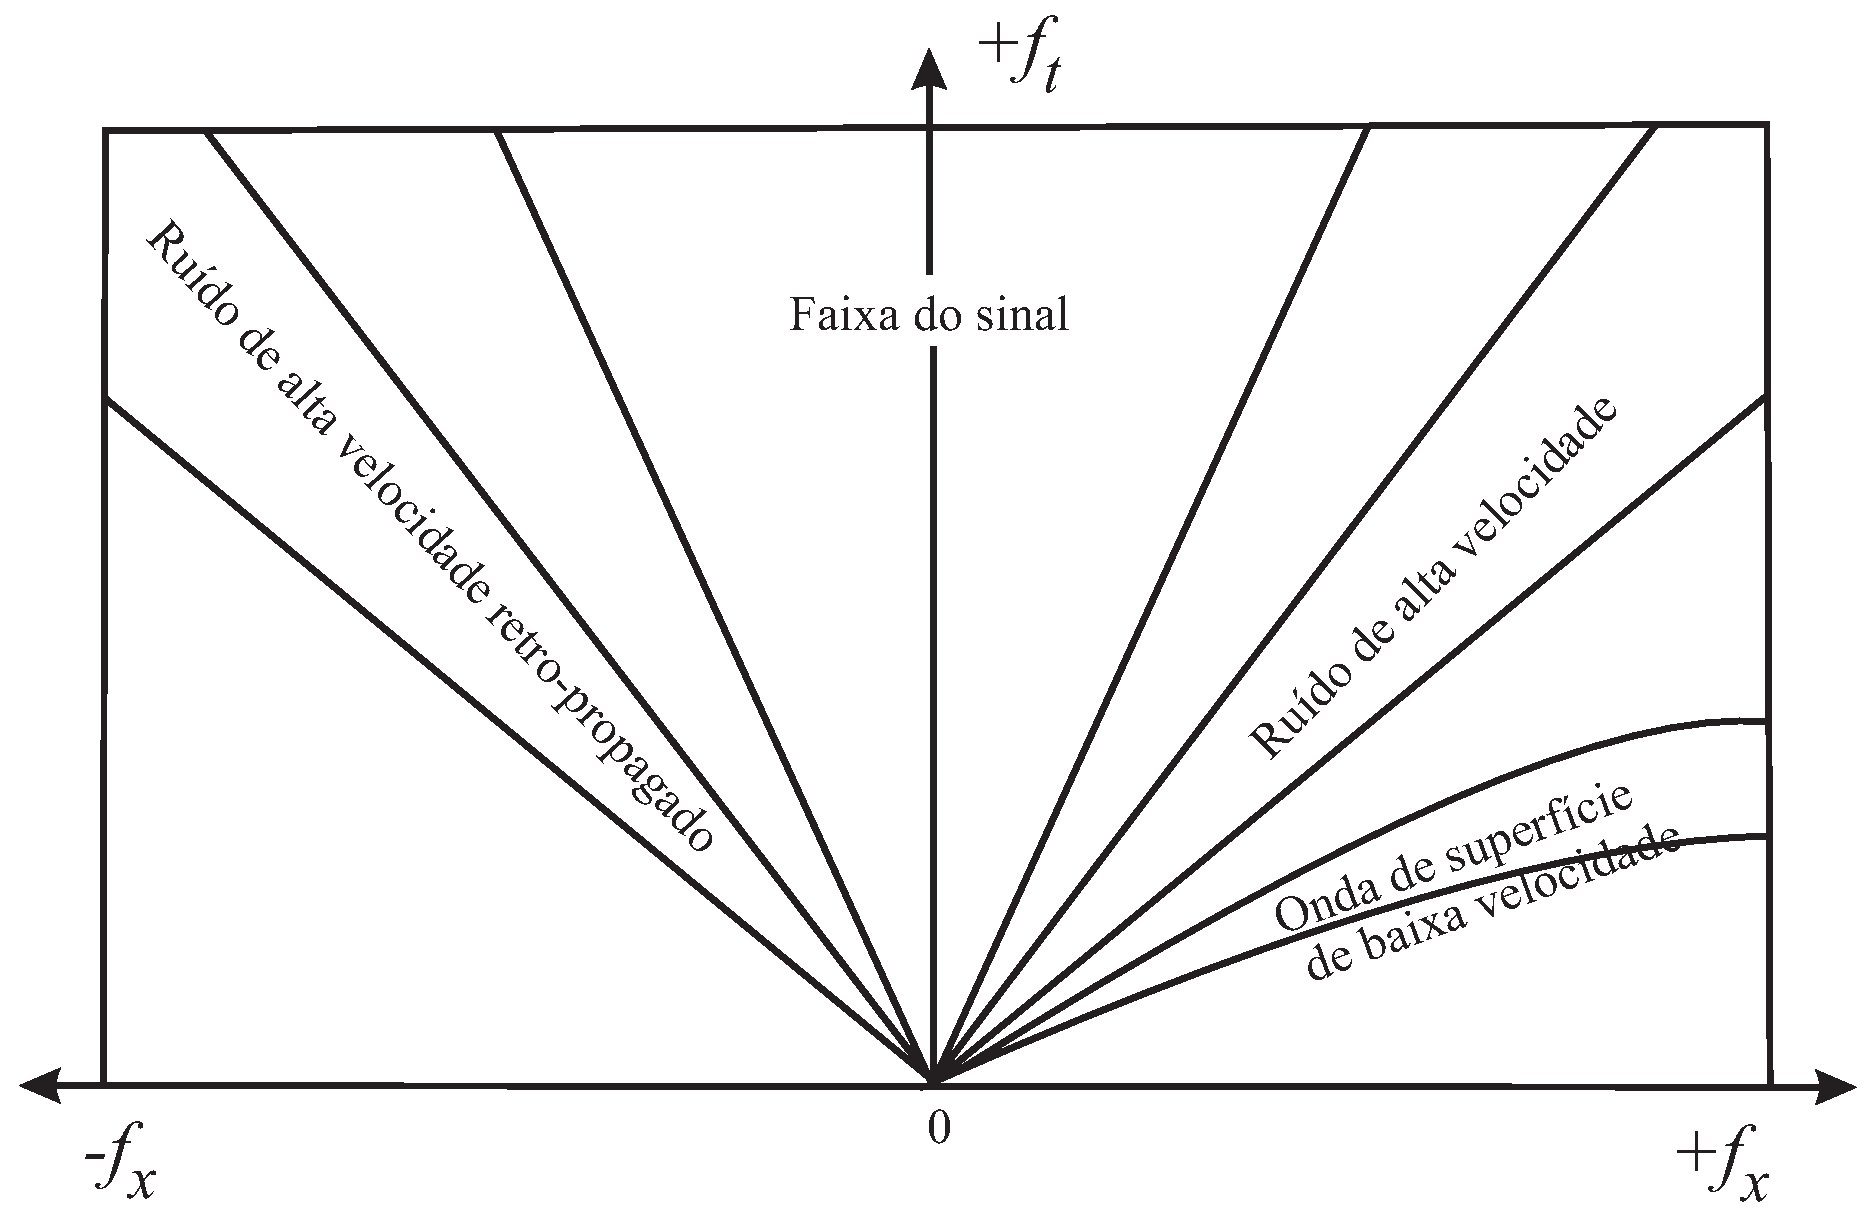
\includegraphics[width=11cm]{figuras/cap2/Analise_Idealizada_Sinal_Ruido_Frequencia.pdf}
\vspace{-0.3cm}
\caption{Ilustração da composição espectral de uma seção sísmica (frequência temporal-espacial). 
Se destacam as linhas de sinal de informação, ruídos de velocidade alta e baixa, e ruido das ondas de superfície de baixa frequência. As linhas inclinadas separam os eventos mergulhantes no domínio $f_{t}-f_{\mathbf{x}}$.}
\label{fig:Analise_Idealizada_Sinal_Ruido_Frequencia}
\end{figure}

A figura \ref{fig:Analise_Idealizada_Filtro_Separa} ilustra o problema que se encontra na tentativa de se aplicar um filtro, $H(f_{t},f_{x})$, convencional simples, o que se ilustra com a figura \ref{fig:Filtro_velocidade}, que tem por finalidade esboçar a relação linear simples (outra forma qualquer pode ser desenhada) no domínio espectral para o caso prático de dados no domínio do discretizado; as frequências de Nyquist estão definidas: 
$f_{Nt}=\frac{1}{2 \Delta t}$, $f_{Nx}=\frac{1}{2 \Delta x}$ e $f_{Nt}= vf_{Nx} =\frac{v}{2 \Delta x}$.
Neste caso, $v$ é a velocidade e $s$ é a vagarosidade.
Observe-se na figura \ref{fig:Filtro_velocidade} as faixas de passagem e de rejeição lineares, onde está superposto uma ilustração de uma linha de contorno típica (forma qualquer) do espectro de um dado real. 
A relação entre as linhas de corte (passagem-rejeição) linear e espectro real não é simples, o que se deseja é que as linha sejam o mais alinhado (paralelo) possível.
%=====================================================
\begin{figure}[H]
\centering
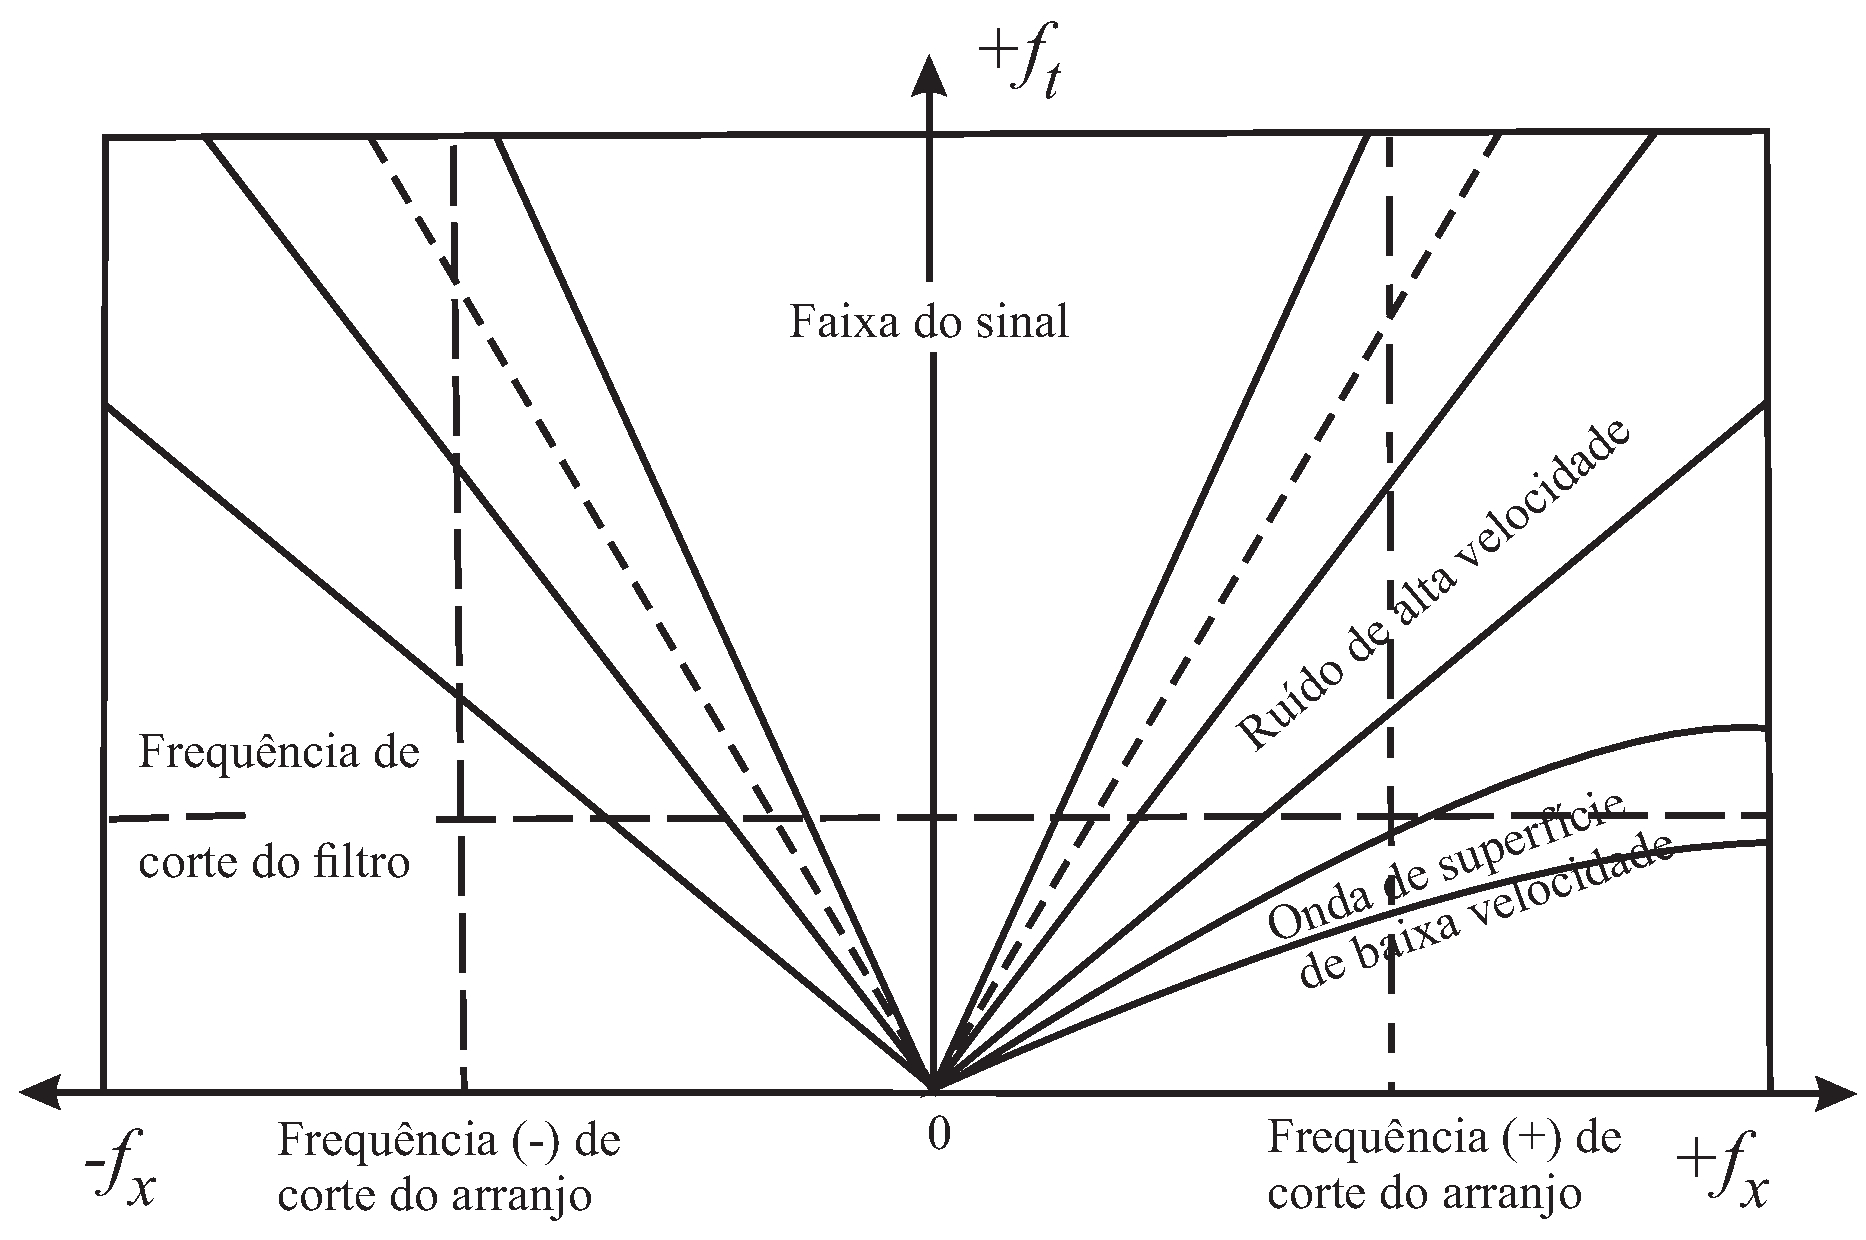
\includegraphics[width=11cm]{figuras/cap2/Analise_Idealizada_Filtro_Separa.pdf}
\vspace{-0.3cm}
\caption{Construção idealizada do filtro para separação da composição espectral de uma seção sísmica (frequência temporal-espacial) correspondente à figura \ref{fig:Analise_Idealizada_Sinal_Ruido_Frequencia}. 
Se destacam as linhas de sinal de informação, ruídos de velocidade alta e baixa, e ruido das ondas de superfície de baixa frequência.}
\label{fig:Analise_Idealizada_Filtro_Separa}
\end{figure}
%=====================================================
%=======================================================
\begin{figure}[H]
\centering
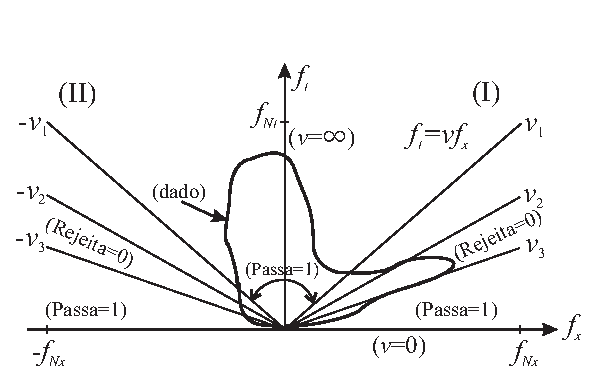
\includegraphics[width=12cm]{figuras/cap2/Filtro_velocidade.pdf}
\vspace{-0.3cm}
\caption{Divisão do domínio da frequência 2D em quadrantes, ilustração do espectro de (dado) real, $H_{R}(f_{t},f_{x})$, e desenho do filtro com a forma Em-leque de Passagem-Rejeição (EL-P-R). 
Para completar o filtro é necessário refletir os quadrantes: I para III e II para IV.}
\label{fig:Filtro_velocidade}
\end{figure}
%=======================================================

A figura \ref{fig:Analise_Idealizada_Filtro_Separa} esboça a tentativa de se preservar uma banda de frequências mais ampla possível. 
Para isto se analisa a geometria do arranjo de registro (padrão de distribuição dos sensores nas estações, padrão de tiro, etc.), e ao passo que as dimensões geométricas do arranjo aumenta, a linha de corte vai no sentido de $f_{x}$ menor (comprimento de onda maior). 
Ao passo que as dimensões do arranjo aumenta, o sistema atenua a informação de eventos de mergulho (linear) e ruído.
E se as dimensões continuam aumentando, o corte passa para o leque do sinal de informação (Faixa do sinal).

Após a aquisição do dado sísmico figura (\ref{fig:afastamento_min}) no $SU$ com o programa \textit{triseis} utilizou-se o tiro $50$ para a filtragem F-K no \textit{matlab}, onde foi implementado os plots da seção tiro figuras \ref{fig:tiro_50}, \ref{fig:tiro_50gain}, \ref{fig:tiro_50ruido} e \ref{fig:tiro_50ruido_gain}. 

O ruído é intrínseco ao registro do traço sísmico, seja como consequência do meio geológico ou do próprio equipamento de registro utilizado. Para simular a entrada de ruído na seção sísmica, assumimos o pressuposto de que ele equivale a um arranjo de números aleatórios de média zero.

\begin{figure}[H]
\centering
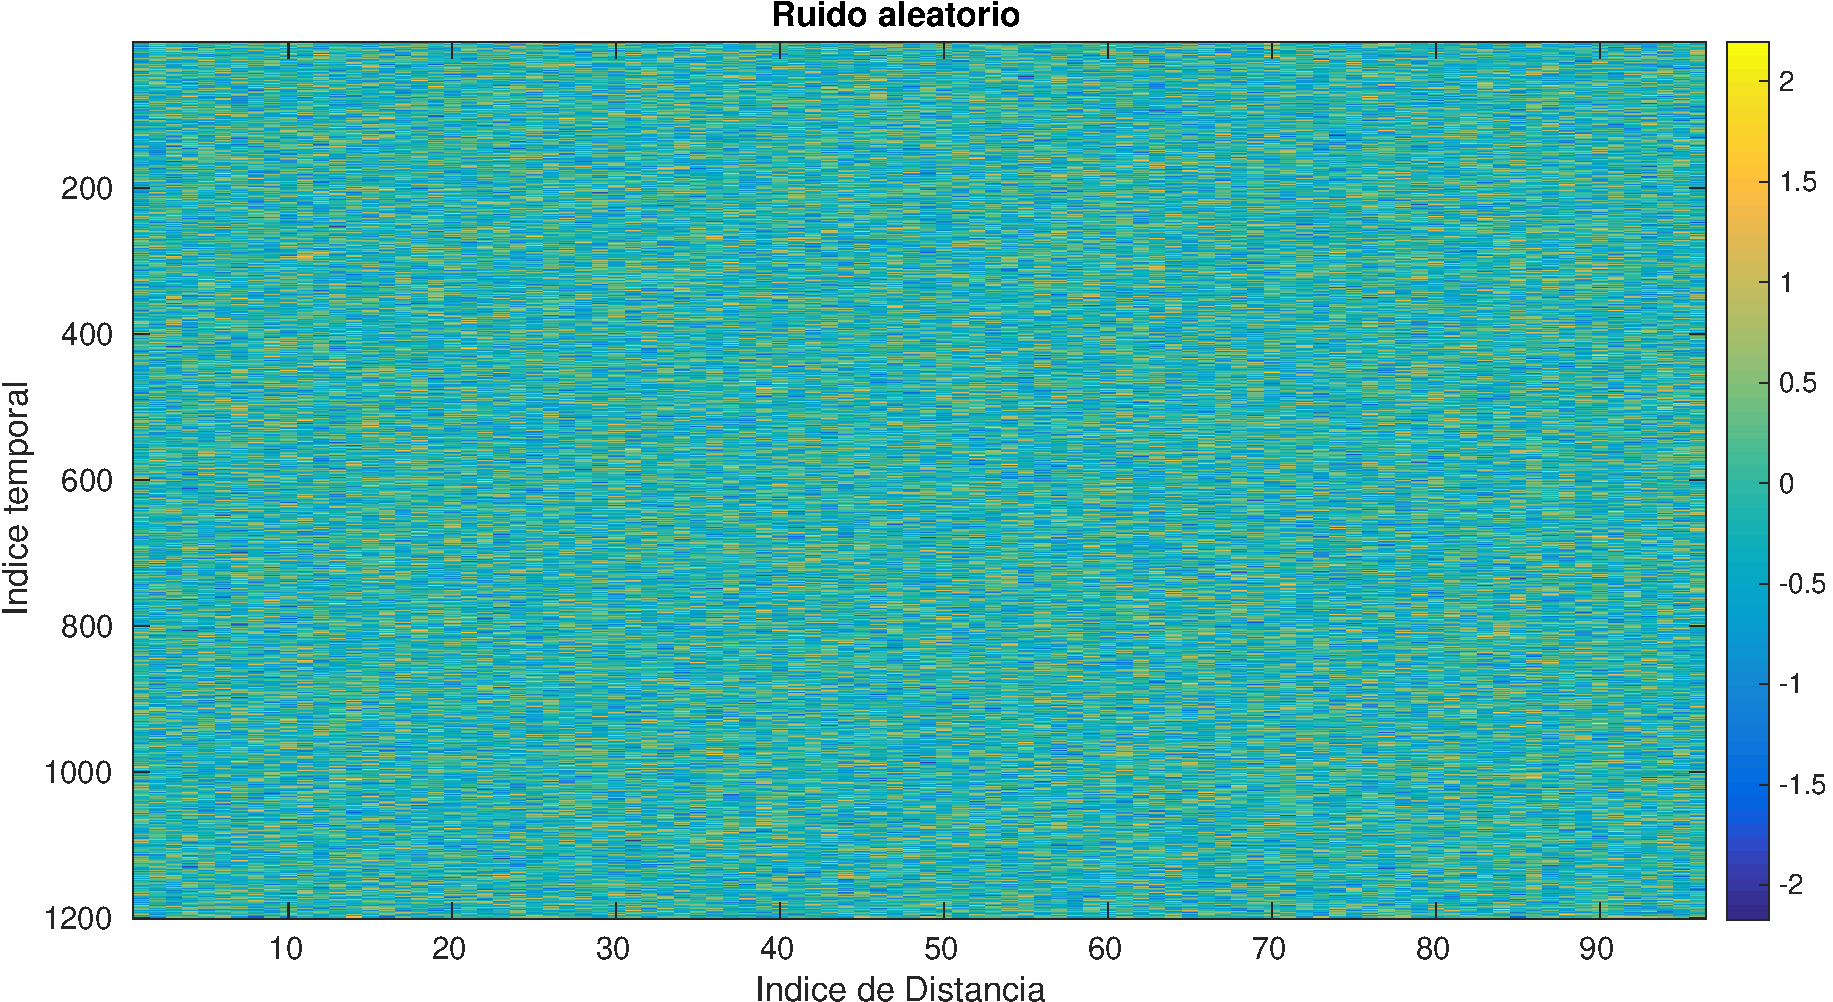
\includegraphics[totalheight=7.0cm]{figuras/cap2/ruido_aletorio.pdf}
\caption{Ruído aleatório gerado no matlab}
\label{fig:ruido_aletorio}
\end{figure}

Nas seções sísmicas se precisa aplicar uma função de ganho devido à diminuição da amplitude com a distância-tempo, denominado de  espalhamento geométrico, divergência esférica, e às vezes atenuação tempo-distância. 
A função ganho empregada corresponde a uma amplificação do sinal no tempo para que se possa ver e interpretar a composição do sinal, que na sísmica é composto de eventos do tipo ruído, reflexões, refrações, múltiplas e difrações. 
Isto é, a correção de espalhamento geométrico por uma função ganho é aplicada para compensar o decaimento de energia da divergência da frente de onda em qualquer fase do processamento de uma seção sísmica. 
Ressalta-se que a aplicação de um ganho é uma operação destrutiva, ou não-destrutiva; o ganho aplicado é classificada como quase não-destrutivo devido ao ponto zero anulado.
A função ganho aplicada é dada por 

\begin{equation}
g(t)=t^{a}e^{-bt},
\label{eq:figura_ganho}
\end{equation}

onde os valores utilizados para os parâmetros foram $a=2$ e $b=0,5$.

\begin{figure}[H]
\centering
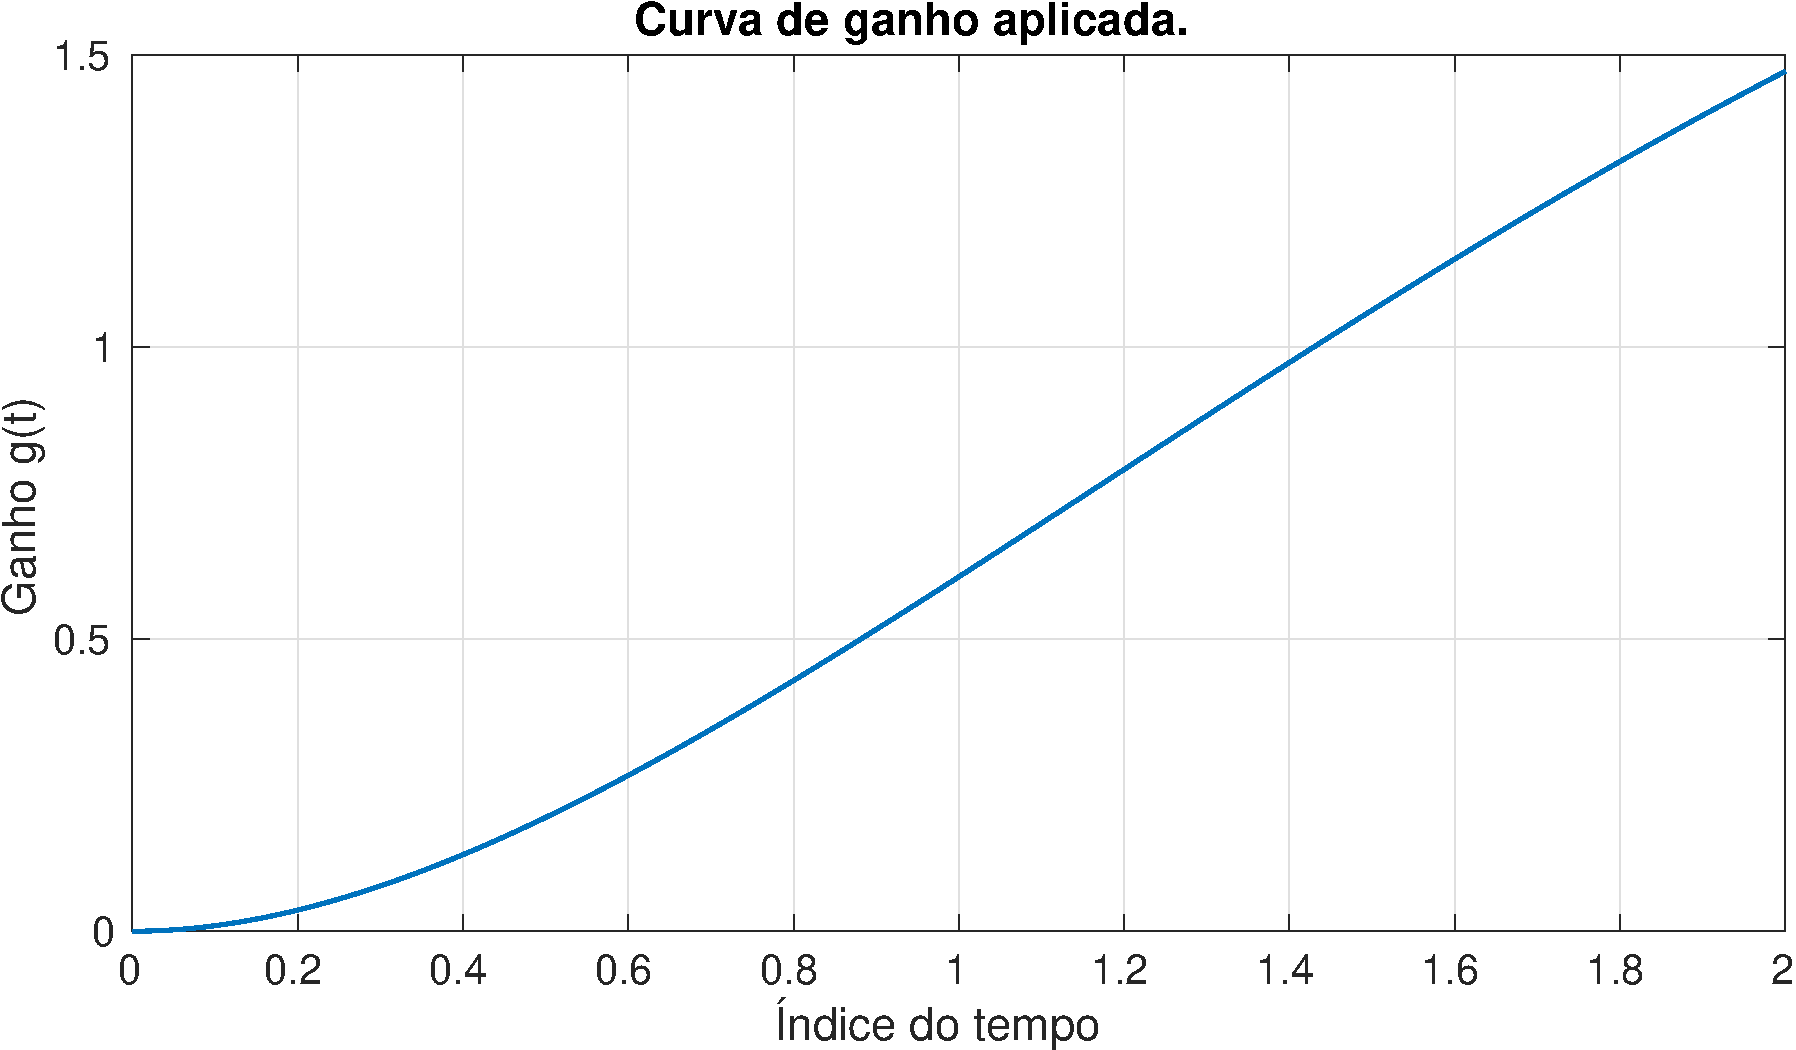
\includegraphics[totalheight=7.0cm]{figuras/cap2/figura_ganho.pdf}
\caption{Função ganho empregada.}
\label{fig:figura_ganho}
\end{figure}

A figura \ref{fig:figura_ganho} mostra a variação do ganho, onde se observa que ela é crescente, mas com um intervalo de amplificação entre zero e $1,5$, que se apresenta de uma forma diferente, mas consistente no que se refere a colocar os valores num intervalo menor.  

Para que se possa realizar uma filtragem, a informação a ser recuperada deve ser separável do não-desejado, no domínio-f , ou no domínio-t.

A figura \ref{fig:espc_tiro50} mostra o espectro de amplitude da seção tiro 50 com ruído gerada a partir da figura \ref{fig:tiro_50ruido}.

O termo filtro é reservado para a operação de multiplicação no domínio da frequência, e pode zerar a parte não desejada do espectro do sinal. Através da definição do espectro de amplitude e de fase podemos construir o operador $H(f)=A(f)e^{\theta(f)}$, que representa o filtro na frequência. Todo e qualquer processo de filtragem de um sinal pode ser representado na seguinte forma:

\begin{equation}
S_{H}(f)=G(f) H(f)
\label{eq:filtragem}
\end{equation}

Onde $S_{H}$ representa o sinal filtrado no domínio da frequência, $G(f)$ representa o sinal a ser filtrado e $H(f)$ o filtro a ser aplicado. Ou no domínio tempo na forma de convolução:

\begin{equation}
s_{h}(t)=s(t) \ast h(t)
\label{eq:filtragem_conv}
\end{equation}

As figuras (\ref{fig:espc_tiro50_c1}), (\ref{fig:espc_tiro50_c2}) e (\ref{fig:espc_tiro50_c3}) ilustram a geometria de passagem e rejeição de uma forma geral.

Após a filtragem da seção tiro 50 (ver figura \ref{fig:secao_filtrada}) nota-se que a maior parte da componente de ruído (informação não desejável) foi removida com a filtragem F-K. O corte no espectro de amplitude de maneira iterativa pelo matlab permite maior precisão na eliminação do ruído. Comparando a figura \ref{fig:secao_filtrada} com \ref{fig:tiro_50ruido}, respectivamente a seção tiro 50 filtrada sem ganho e seção tiro 50 com ruído.

Em seguida a figura \ref{fig:secao_filtrada_gain} mostra a atuação do ganho na seção tiro 50 filtrada, o ganho aumenta com o tempo ou seja não apenas os eventos desejavéis são amplificados como também a componente de ruído. Comparando as duas figura \ref{fig:secao_filtrada_gain} com \ref{fig:tiro_50ruido_gain} onde respectivamente representam a seção tiro 50 filtrada com ganho e seção tiro 50 com ruído e ganho.

\begin{landscape}
\begin{figure}[H]
\centering
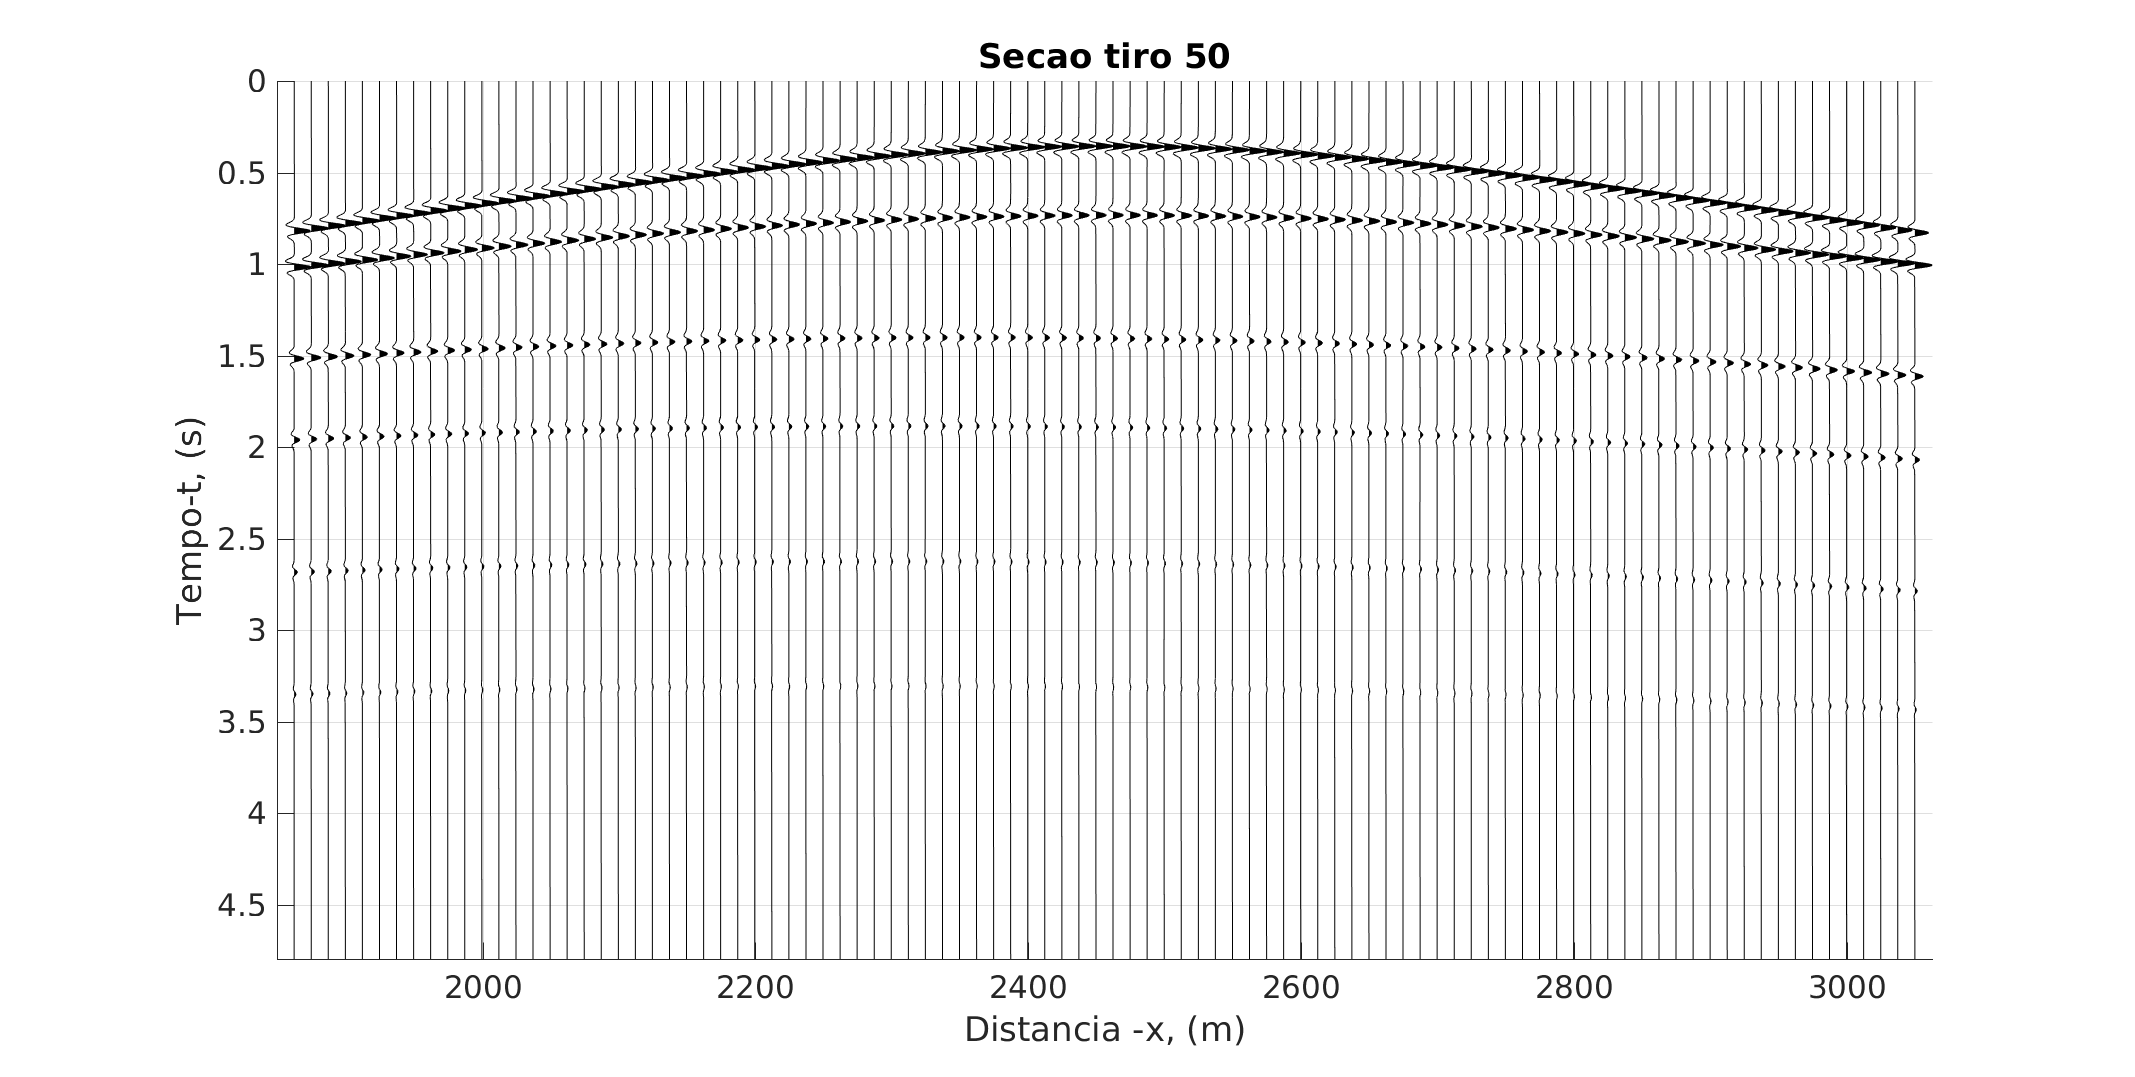
\includegraphics[totalheight=14cm]{figuras/cap2/secao_tiro50.pdf}
\caption{Seção tiro 50 sem ganho do modelo sintético, figura (\ref{fig:vagarosidade})}
\label{fig:tiro_50}
\end{figure}
\end{landscape}

\begin{landscape}
\begin{figure}[H]
\centering
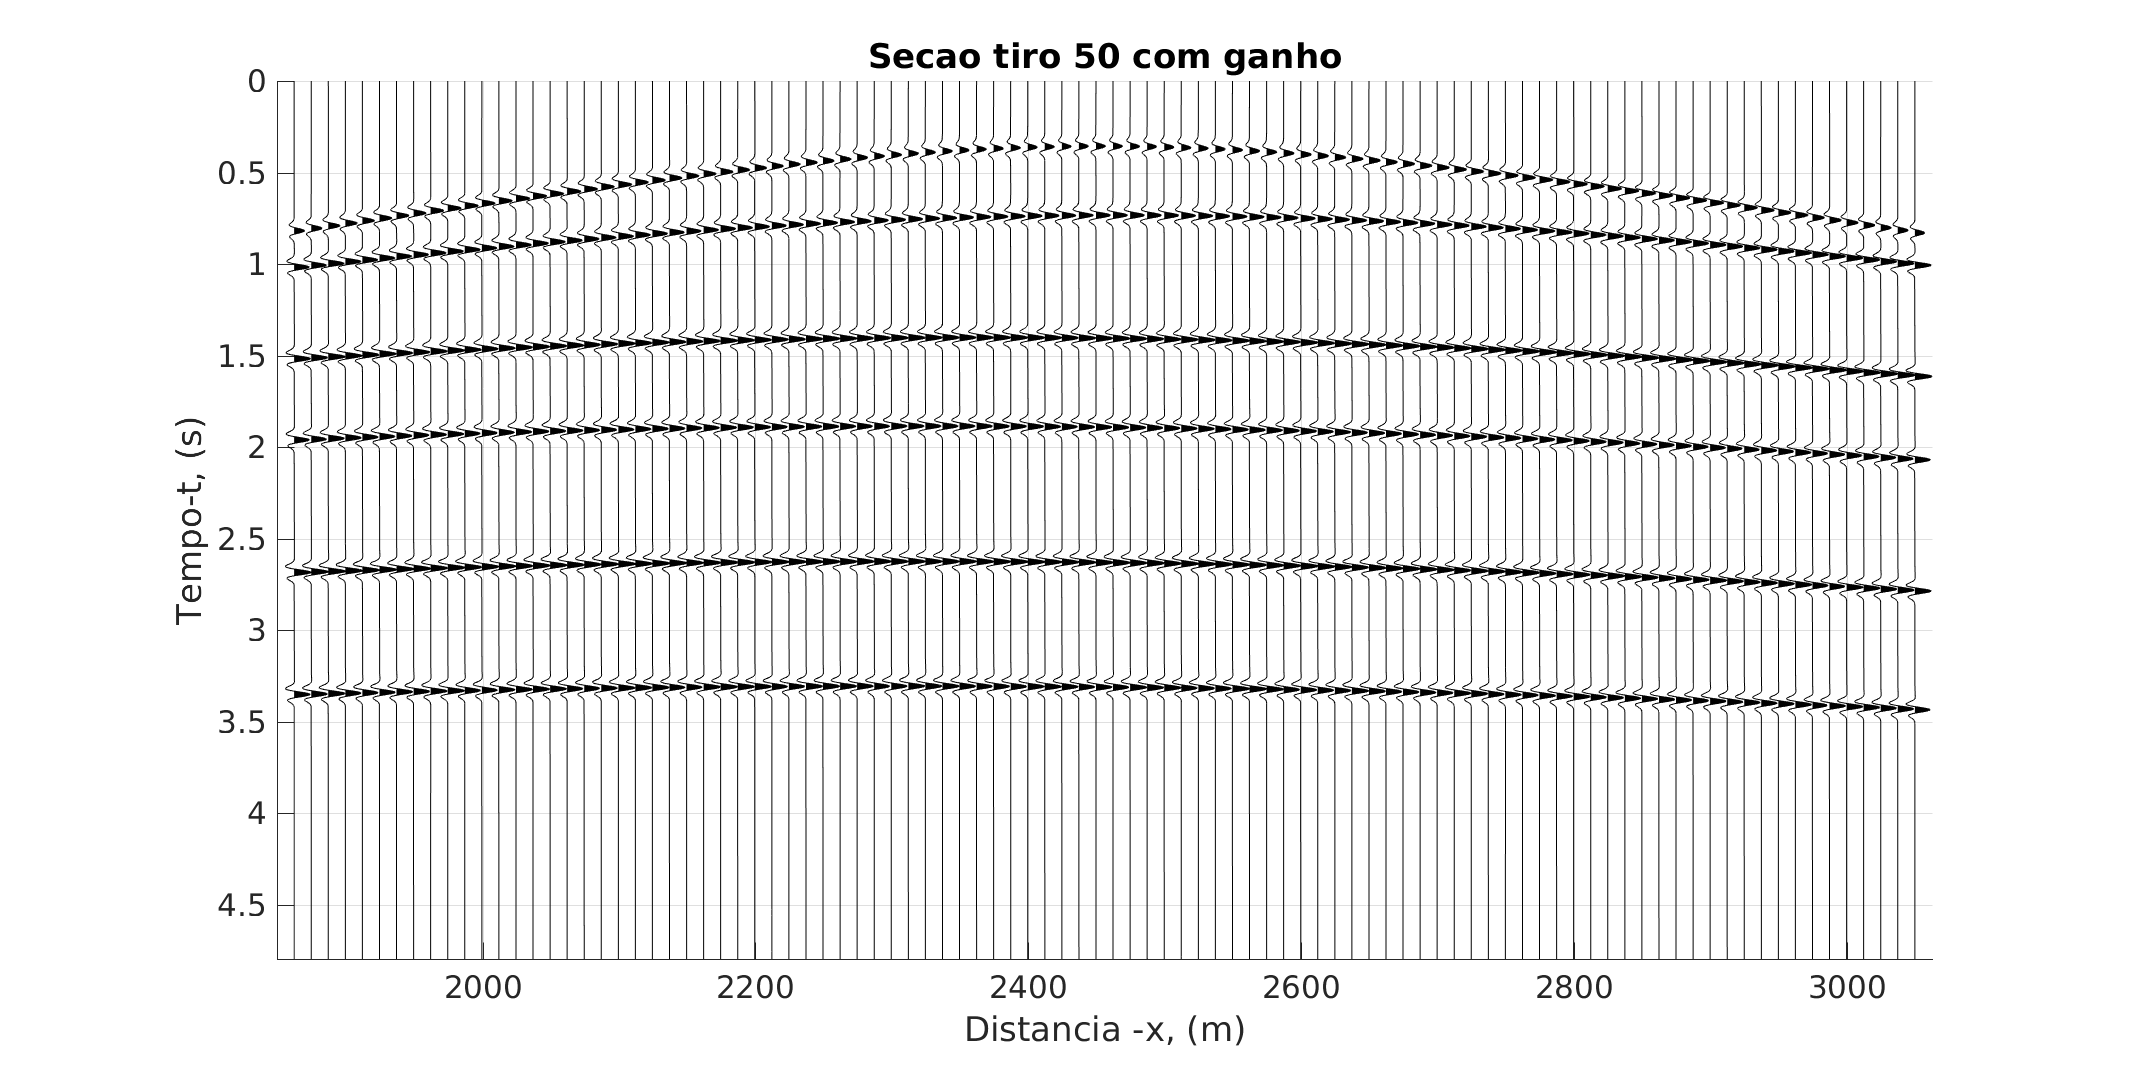
\includegraphics[totalheight=14cm]{figuras/cap2/secao_tiro50_ganho.pdf}
\caption{Seção tiro 50 com ganho, os eventos com maior tempo foram realçados.}
\label{fig:tiro_50gain}
\end{figure}
\end{landscape}

\begin{landscape}
\begin{figure}[H]
\centering
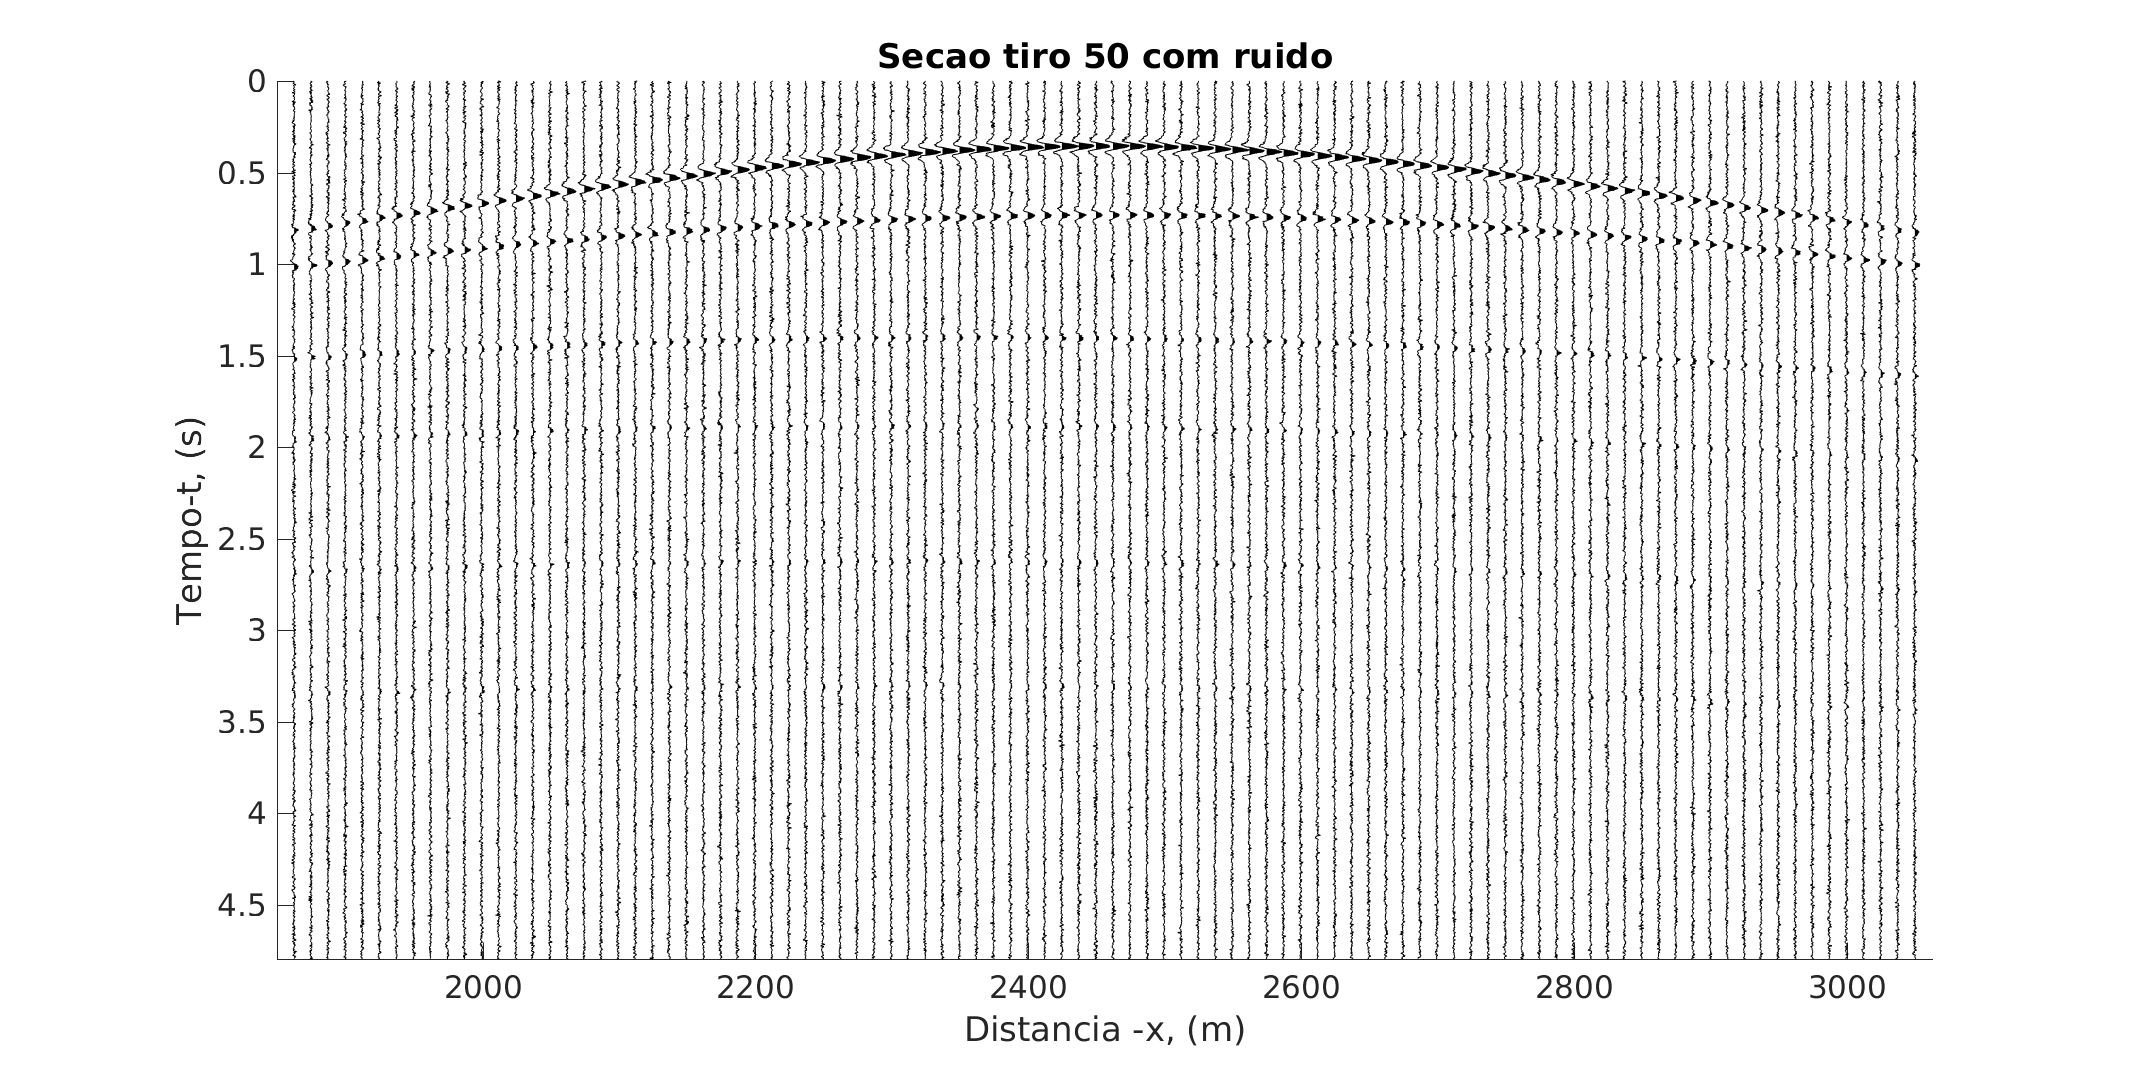
\includegraphics[totalheight=14cm]{figuras/cap2/secao_tiro50_ruido.pdf}
\caption{Seção tiro 50 com ruido aleatório, o ruído foi gerado no matlab e somado a seção tiro 50.}
\label{fig:tiro_50ruido}
\end{figure}
\end{landscape}

\begin{landscape}
\begin{figure}[H]
\centering
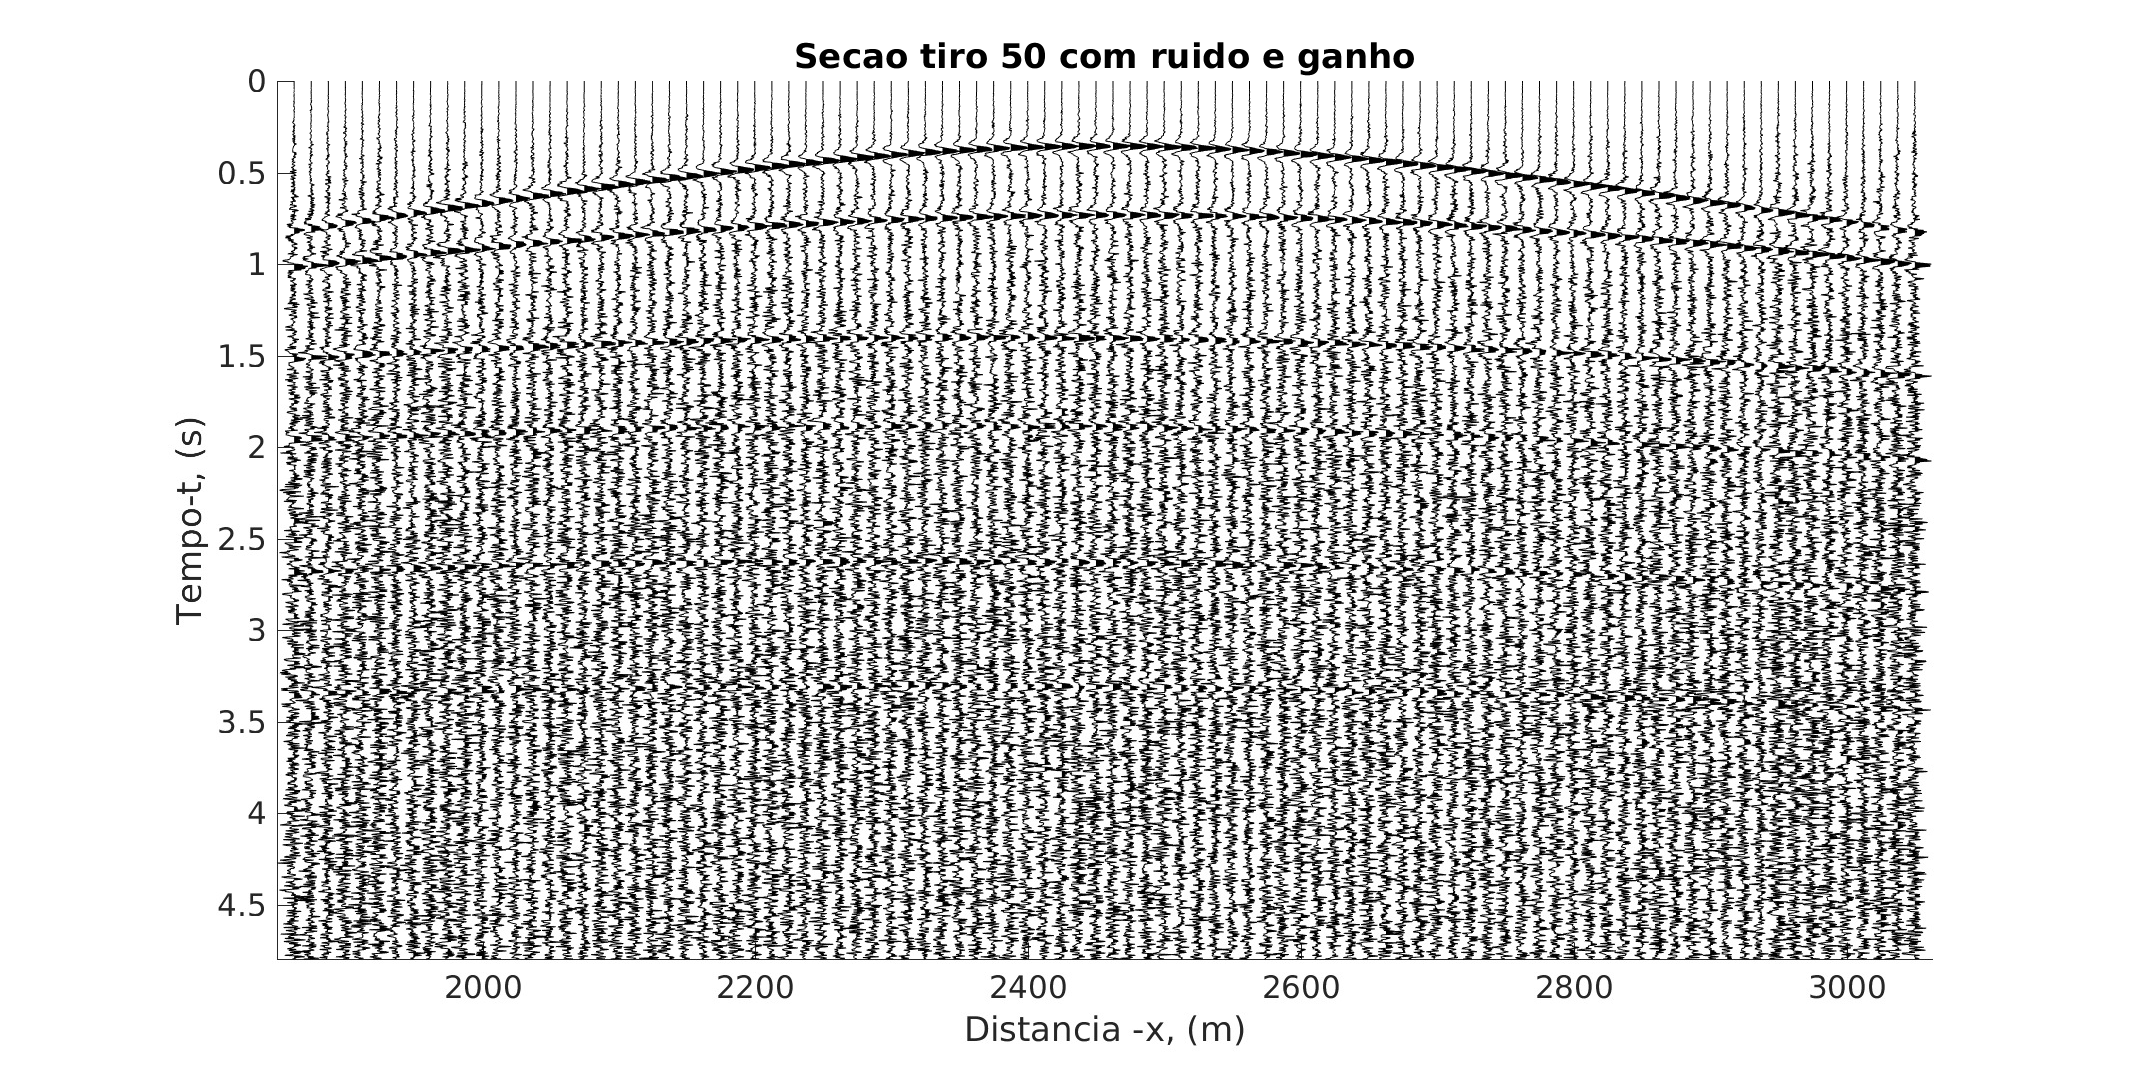
\includegraphics[totalheight=14cm]{figuras/cap2/secao_tiro50_ruido_gain.pdf}
\caption{Seção tiro 50 com ruido e ganho, a informação e o ruído foram amplificados, os eventos de maior tempo foram ``mascarados'' com a amplificação da função ganho.}
\label{fig:tiro_50ruido_gain}
\end{figure}
\end{landscape}

\begin{landscape}
\begin{figure}[H]
\centering
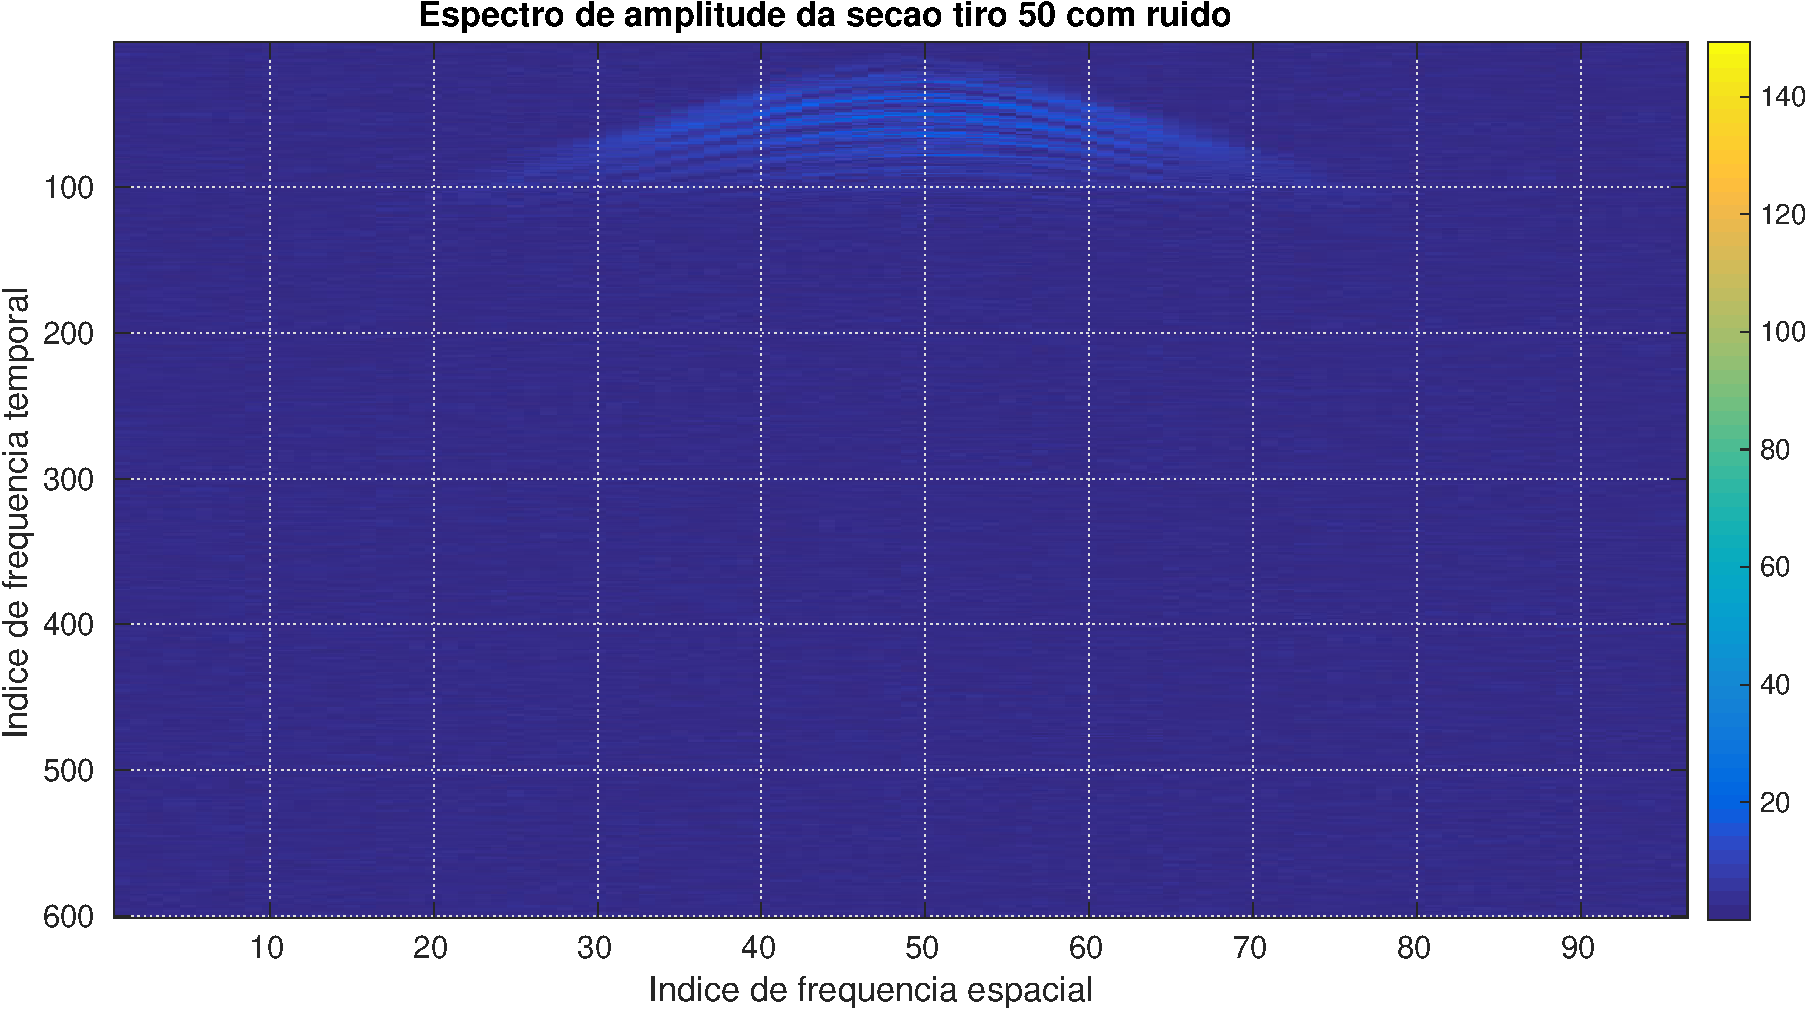
\includegraphics[totalheight=14cm]{figuras/cap2/espc_tiro50.pdf}
\caption{Espectro da seção tiro 50 com ruído, este espectro não apresenta falseamento de informação tanto em $f_t$ (frequência temporal) quanto em $f_k$ (frequência espacial).}
\label{fig:espc_tiro50}
\end{figure}
\end{landscape}

\begin{landscape}
\begin{figure}[H]
\centering
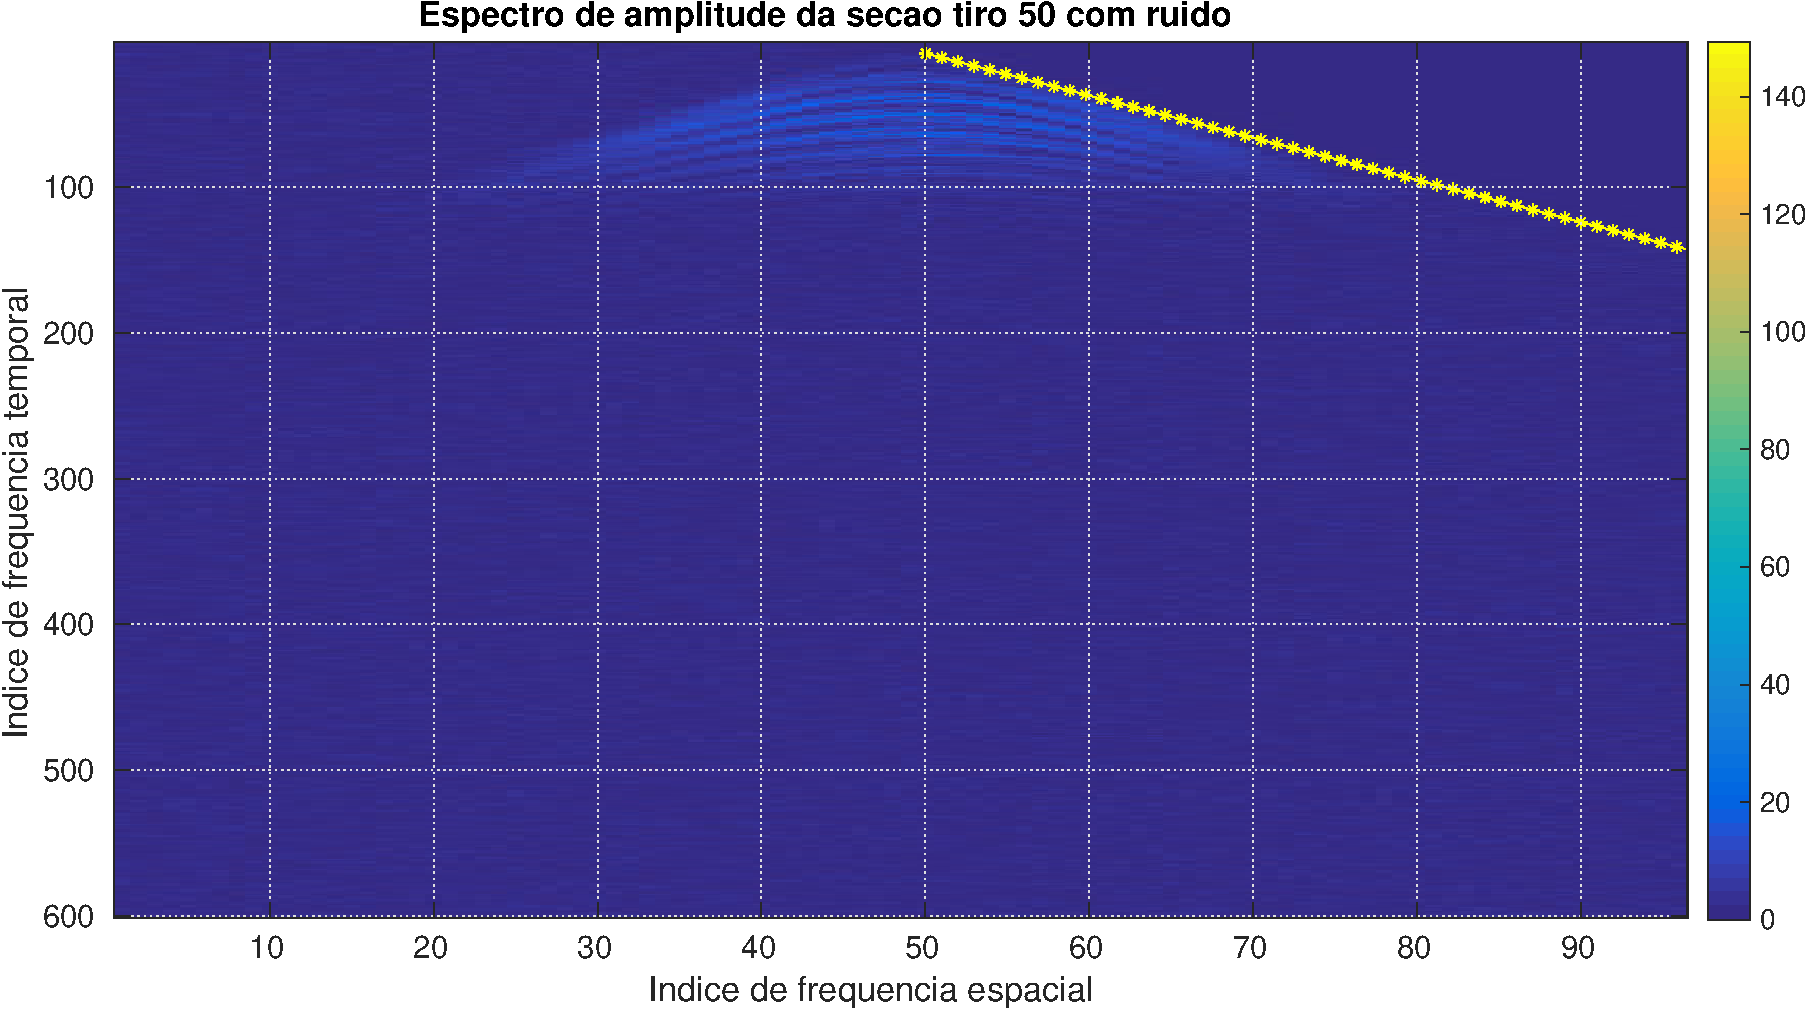
\includegraphics[totalheight=14cm]{figuras/cap2/espc_tiro50_c1.pdf}
\caption{Seção tiro 50 com ruído após o primeiro corte (linha amarela) no espectro de amplitude.}
\label{fig:espc_tiro50_c1}
\end{figure}
\end{landscape}

\begin{landscape}
\begin{figure}[H]
\centering
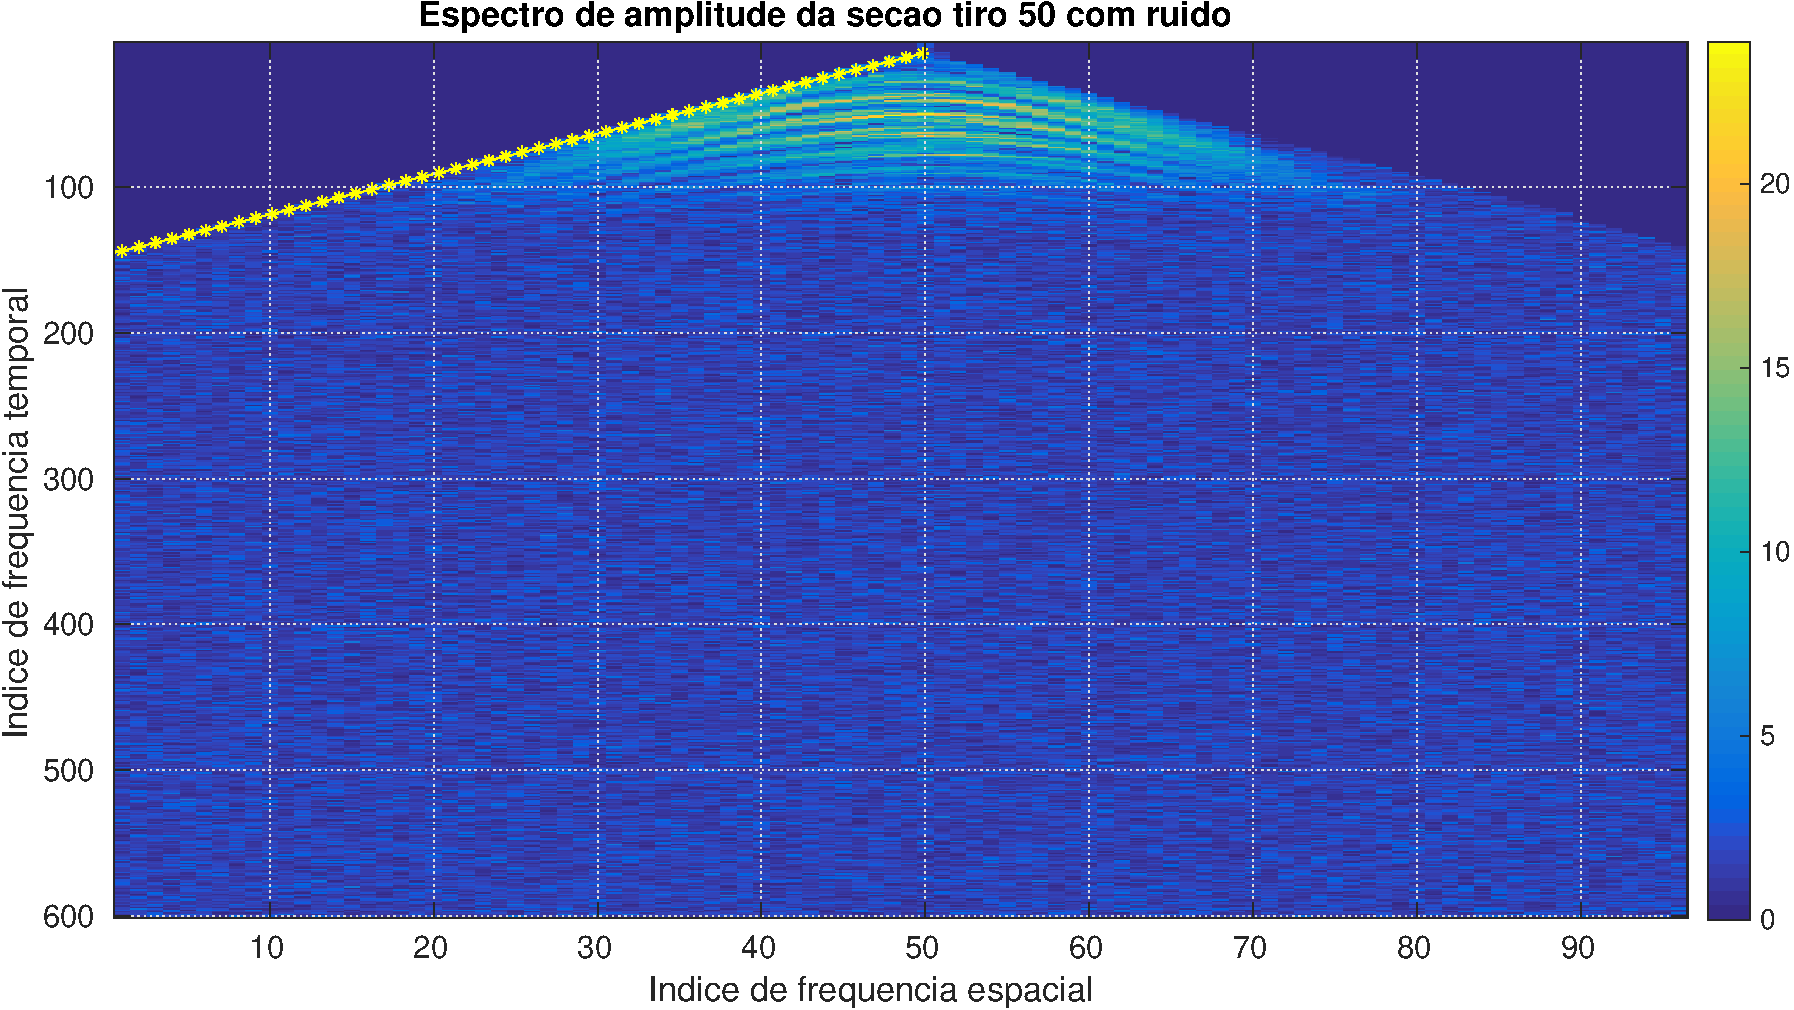
\includegraphics[totalheight=14cm]{figuras/cap2/espc_tiro50_c2.pdf}
\caption{Seção tiro 50 com ruído após o segundo corte (linha amarela) no espectro de amplitude.}
\label{fig:espc_tiro50_c2}
\end{figure}
\end{landscape}

\begin{landscape}
\begin{figure}[H]
\centering
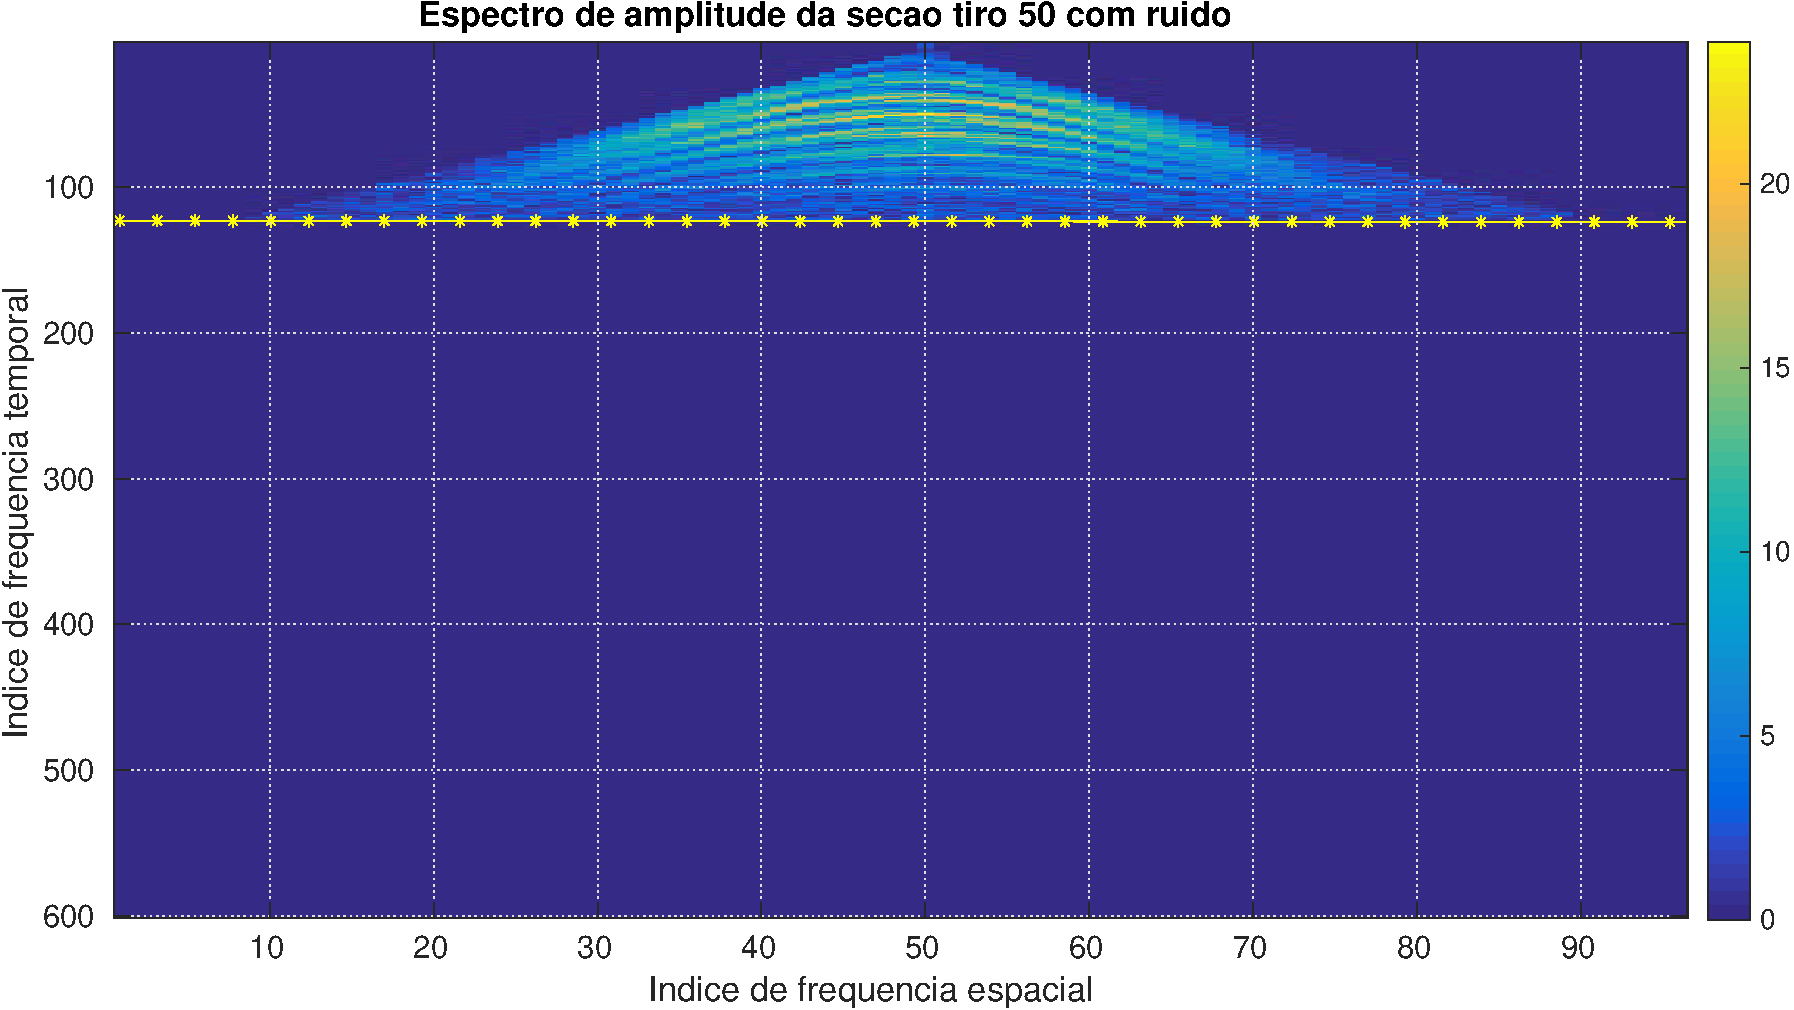
\includegraphics[totalheight=14cm]{figuras/cap2/espc_tiro50_c3.pdf}
\caption{Seção tiro 50 com ruído após o terceiro corte (linha amarela) no espectro de amplitude.}
\label{fig:espc_tiro50_c3}
\end{figure}
\end{landscape}

\begin{landscape}
\begin{figure}[H]
\centering
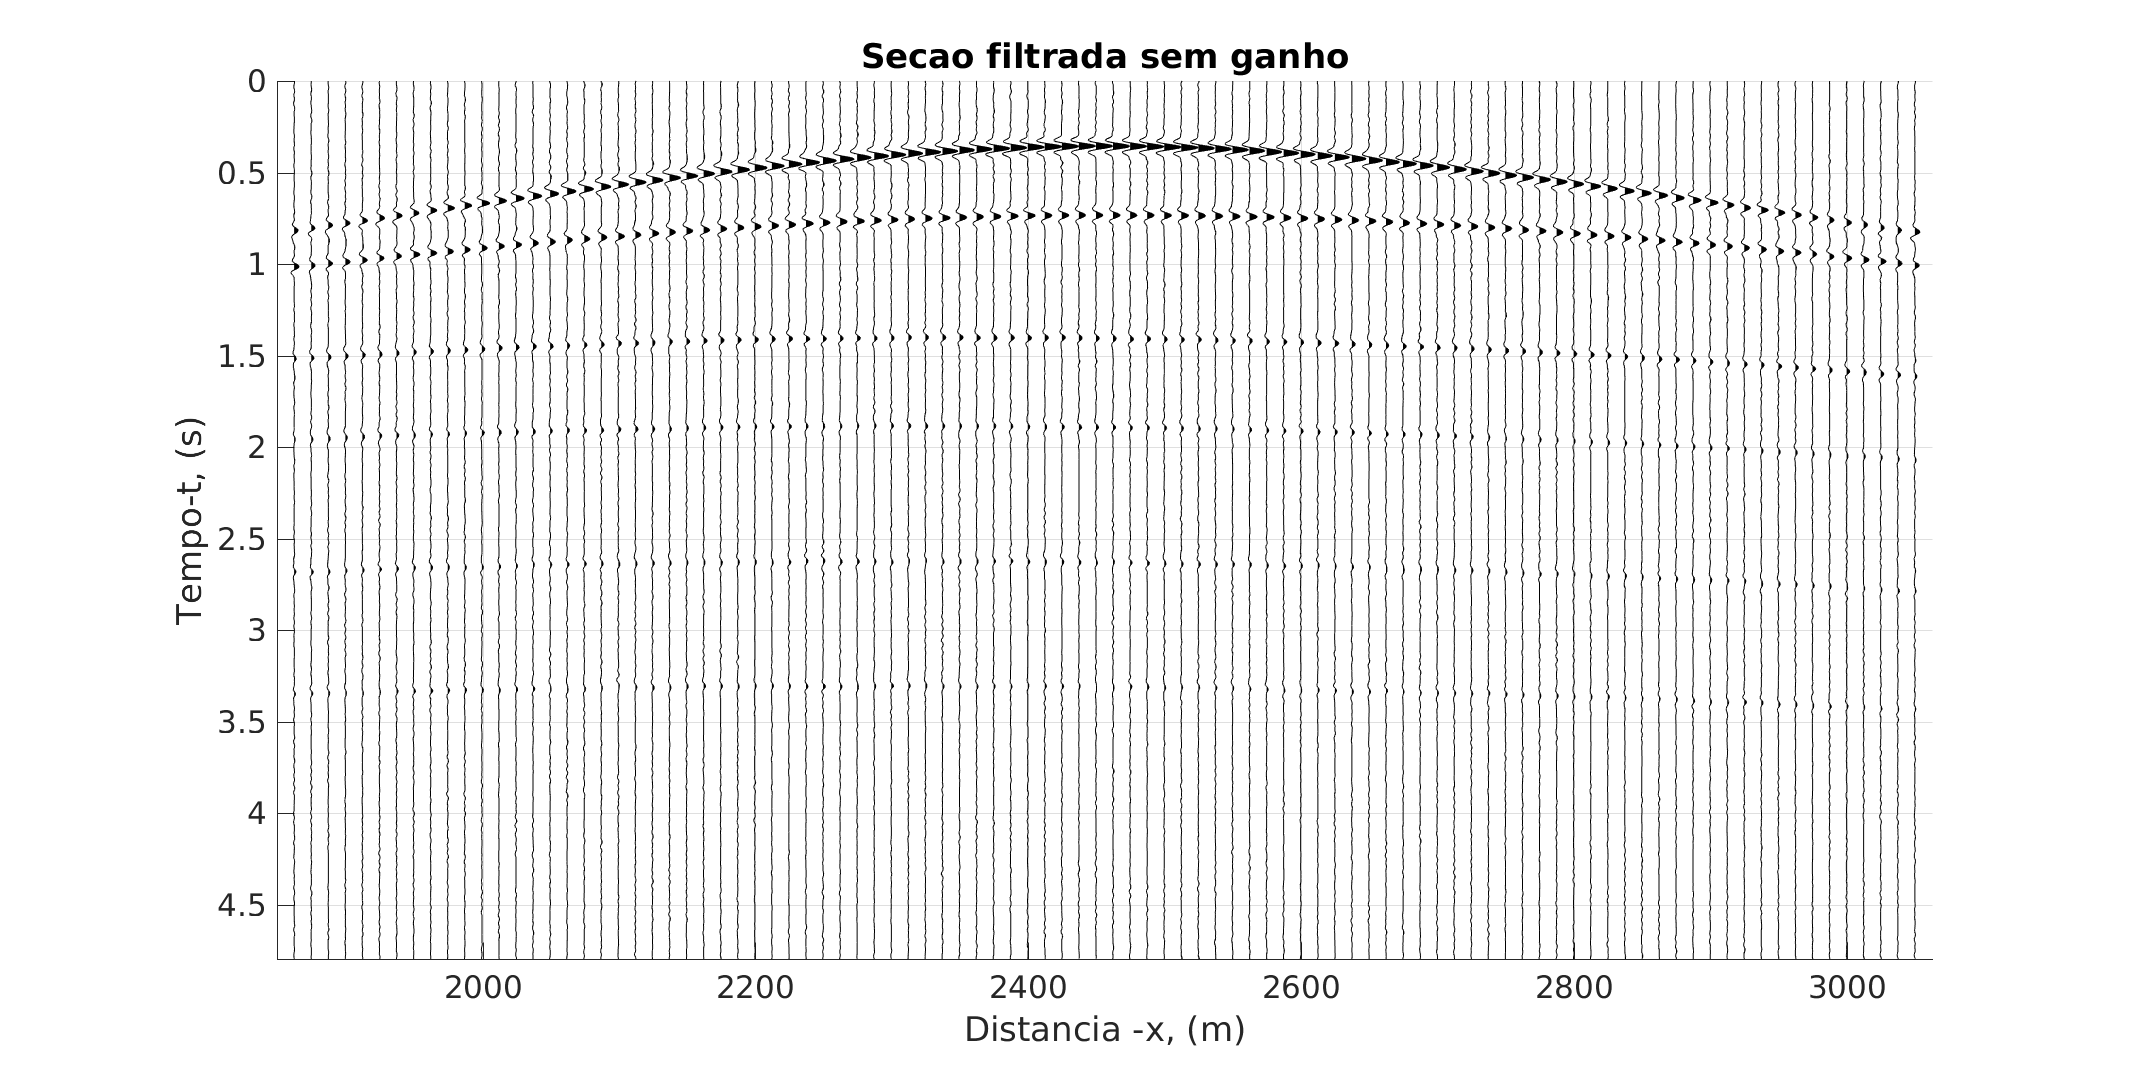
\includegraphics[totalheight=14cm]{figuras/cap2/secao_filtrada.pdf}
\caption{Seção tiro 50 filtrada do ruído sem ganho, comparando a figura (\ref{fig:tiro_50ruido}) nota-se que a componente do ruído foi em grande parte removida após a filtragem F-K.}
\label{fig:secao_filtrada}
\end{figure}
\end{landscape}

\begin{landscape}
\begin{figure}[H]
\centering
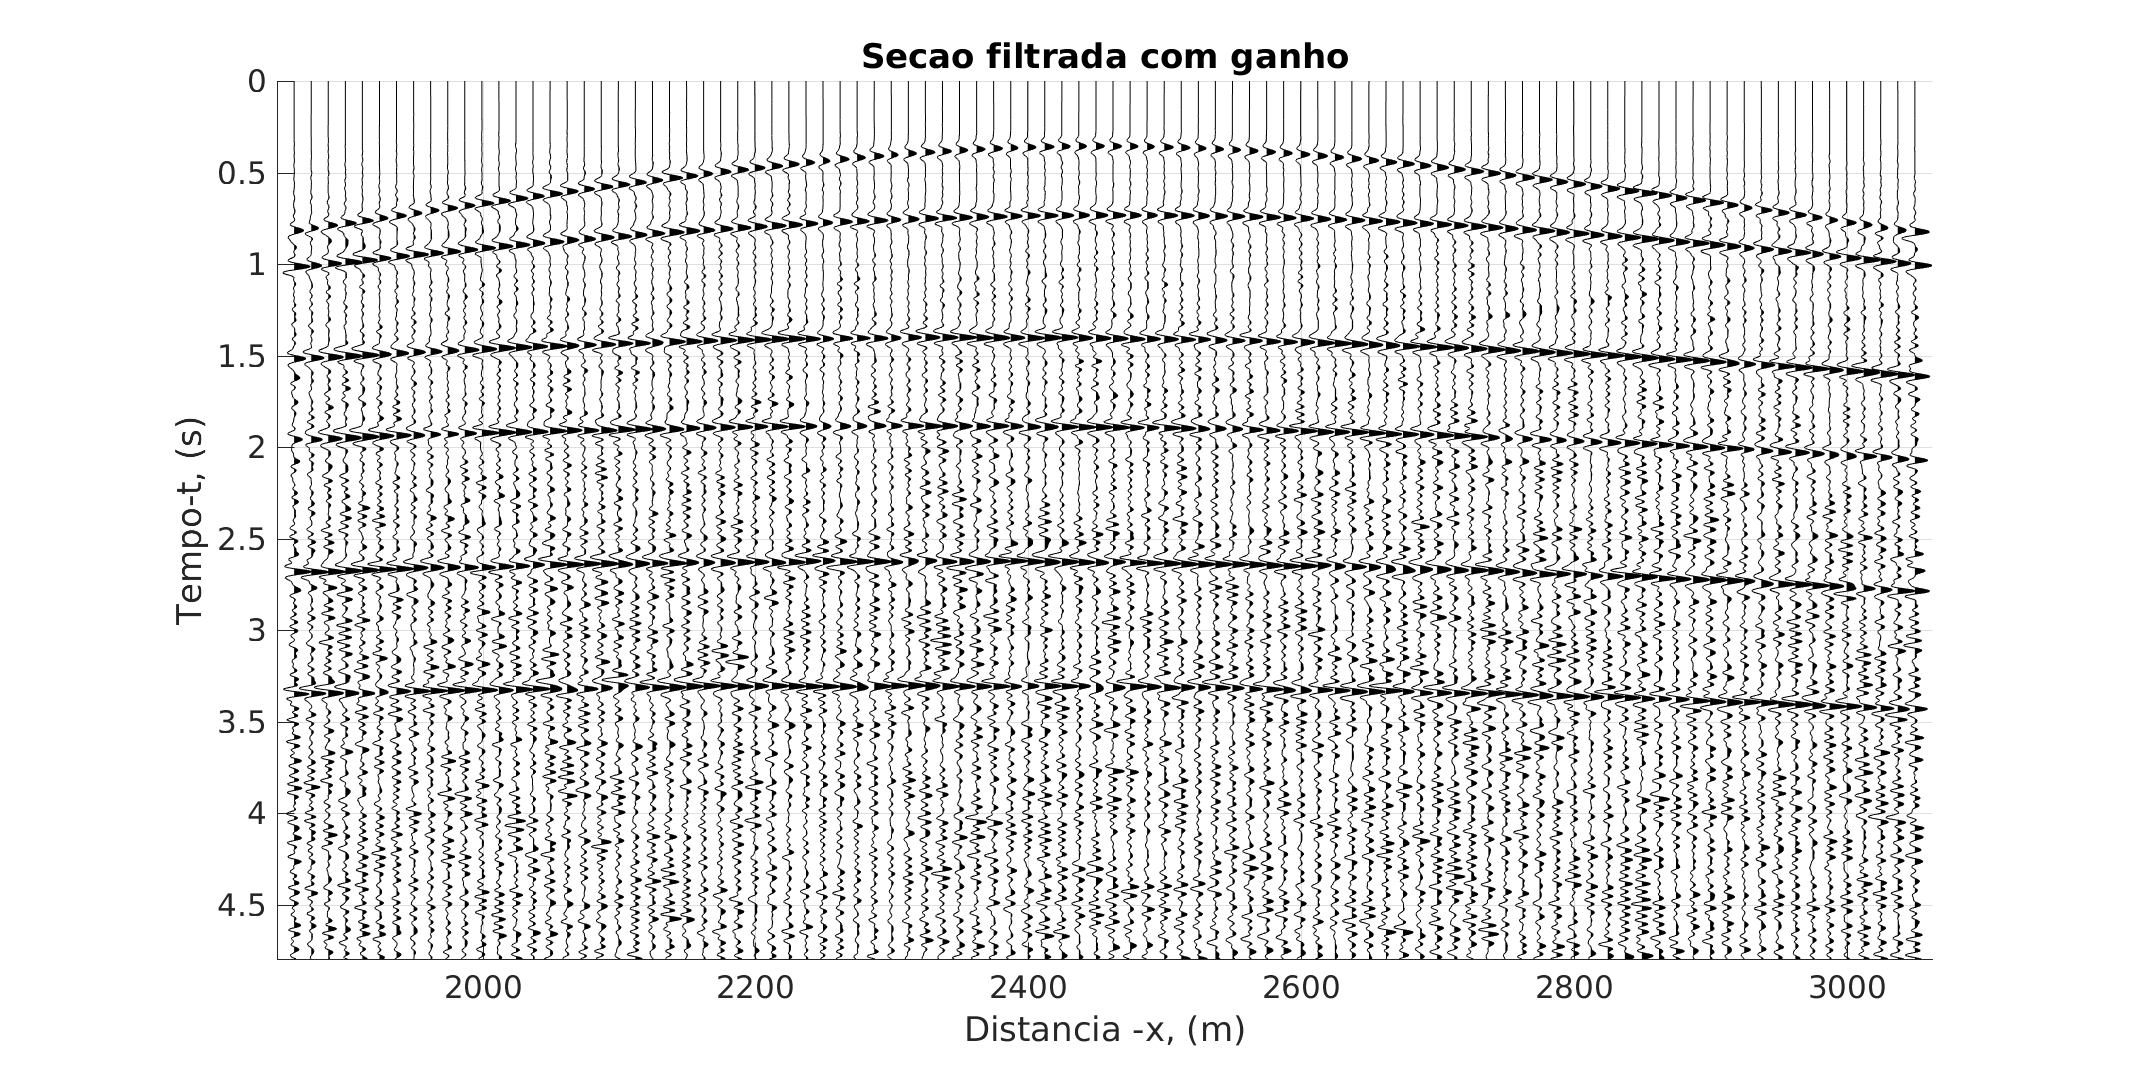
\includegraphics[totalheight=14cm]{figuras/cap2/secao_filtrada_gain.pdf}
\caption{Seção tiro 50 filtrada do ruído com ganho, comparando a figura (\ref{fig:tiro_50ruido_gain}) nota-se que os eventos com maior tempo foram recuperados. O ganho amplificou tanto a informação de interesse (eventos) quanto o ruído.}
\label{fig:secao_filtrada_gain}
\end{figure}
\end{landscape}

\section{COBERTURA MÁXIMA DOS CDP'S}

Após o carregamento da geometria, uma forma de saber se a aquisição foi satisfatória é fazer plots de seções de afastamento constante, tais como a seção de afastamento mínimo (ver figura \ref{fig:afastamento_min}), médio e máximo, visualizar alguns CDPs para conferir as coordenadas ou qualquer família desejada.

Uma importante etapa para processos posteriores é a visualização da família de CDPs para analisar quais possuem cobertura máxima. Está etapa está diretamente relacionada a com a análise de velocidade do dado sísmico. Para iniciar a análise de velocidade, o dado de entrada deve estar organizado (sorteado) em famílias de CDPs. O programa susort (ver anexo) é um programa do SU que faz esse sorteamento de forma rápida. 

A figura \ref{fig:geometria_cdp} mostra a superposição das coordenadas tiro-receptor (s, g), ponto médio-afastamento (y, h) e geometrias do traçamento de raios para vários tipos de ``coleta'' (gather). As coordenadas (y, h) foram rotacionadas $45^{\circ}$ em relação às coordenadas (s, g). A área pontilhada representa a cobertura usada no registro do perfil sísmico ao longo do eixo do ponto médio, $Oy$.
Cada ponto representa um traço sísmico com o eixo do tempo perpendicular ao plano do papel.

O comprimento do cabo de gravação é representado pelo segmento $FG$ e o comprimento da linha é $AD$. O número de pontos ao longo do eixo de afastamento (seção transversal 3) é igual à cobertura máxima CDP. A cobertura máxima diminui nas extremidades do perfil (segmentos $AB$
e $CD$). A cobertura máxima completa ao longo da linha está nos pontos médios do segmento $BC$. O diagrama da \ref{fig:geometria_cdp} é conhecido como gráfico de empilhamento e é útil ao configurar a geometria de uma linha para pré-processamento. Se faltar um tiro ou um receptor ruim, os pontos médios afetados são facilmente identificados. Para a maioria das geometrias de gravação, a cobertura máxima $n_f$ para um CDP é fornecida por:

\begin{eqnarray}
n_{f}&=&\frac{n_{g}\Delta g}{2\Delta s},\\
\nonumber &=&\frac{96*25}{2*50},\\ 
\nonumber &=& 24
\label{eq:cobertura_max}
\end{eqnarray}

Onde $\Delta g$ e $\Delta s$ são os intervalos do grupo de receptores e dos disparos, respectivamente, e $n_g$ é o número de canais de gravação.

O gráfico de cobertura máxima (figura \ref{fig:CDPiluminados}) pode ser gerado a partir do programa sukeycount onde o parâmetro de entrada é a chave CDP e o dado sísmico (ver anexo), com o auxilio do matlab gera-se o gráfico de cobertura máxima que indica quais CDPs serão posteriormente utilizados na análise de velocidade.

\begin{figure}[H]
\centering
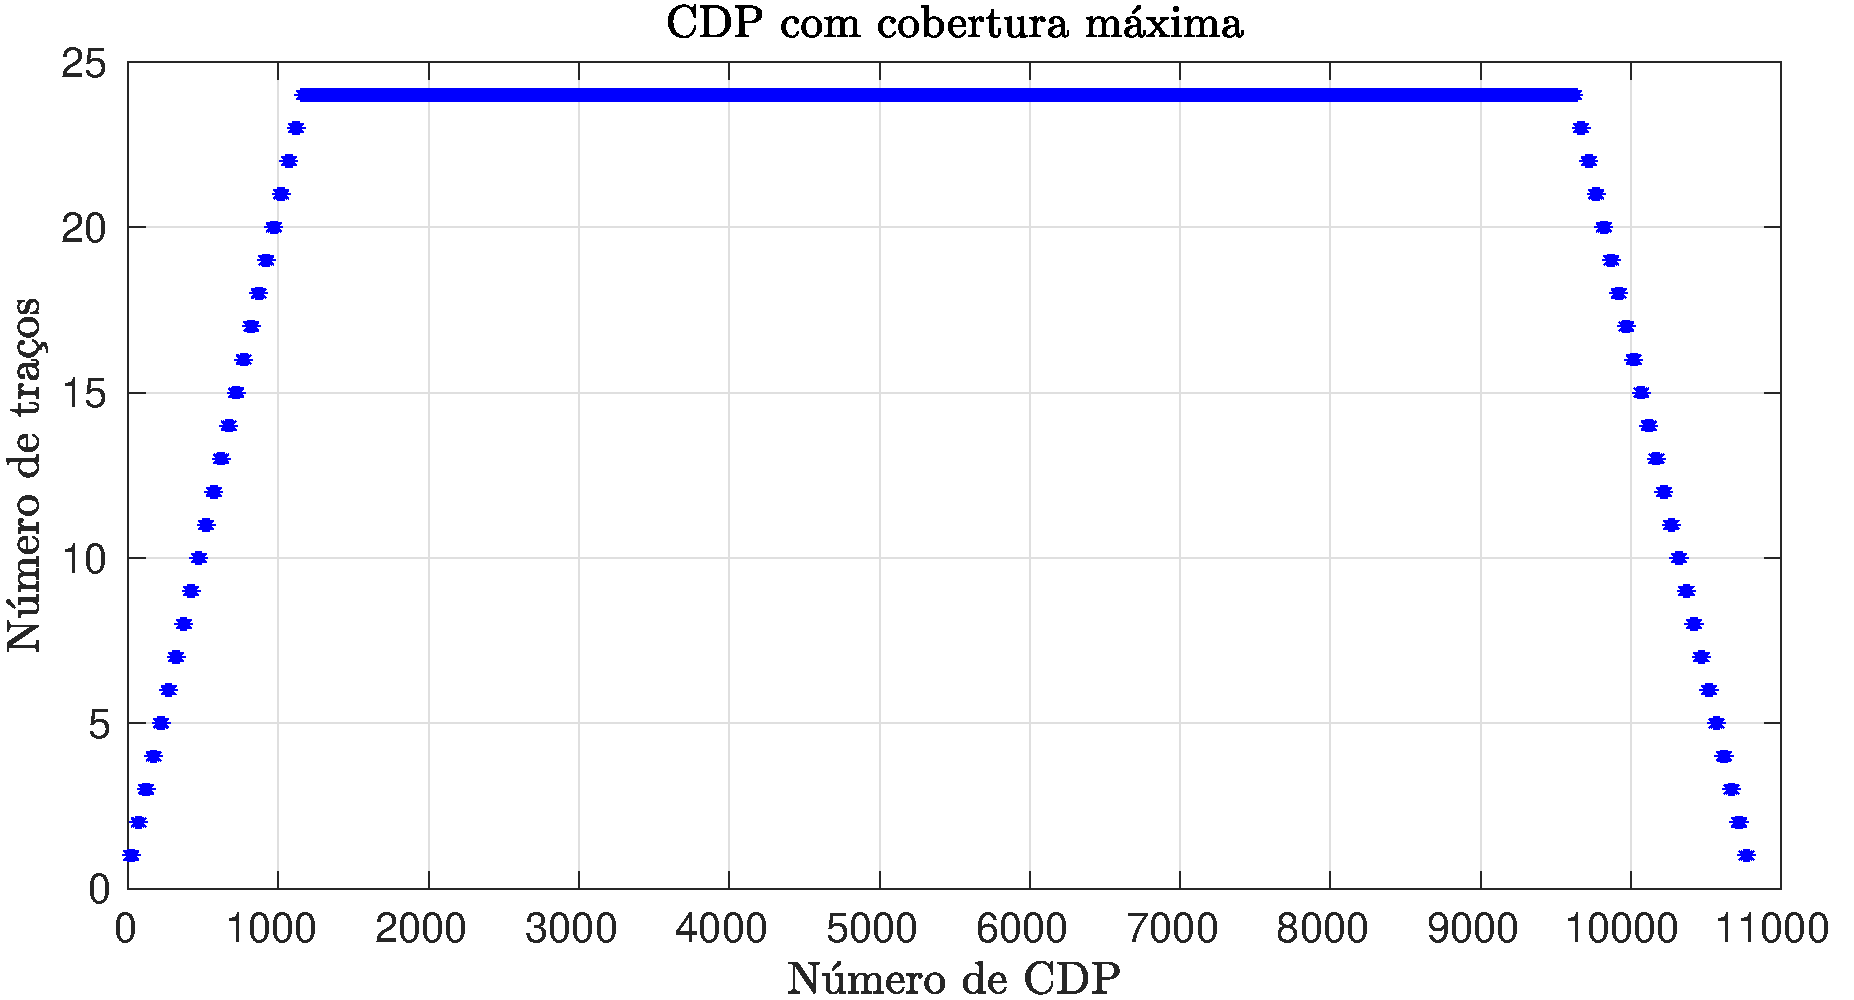
\includegraphics[width=16cm]{figuras/cap2/CDP_iluminados.pdf}
\caption{Máxima cobertura de família CDPs entre o CDP de número 1150 e 9650. No intervalo de cobertura máxima o número de traços é 24 por CDP.}
\label{fig:CDPiluminados}
\end{figure}

A equação que descreve o tempo de trânsito para uma reflexão de uma família CDP tem a seguinte forma:

\begin{equation}
t^{2}={t_0}^2+\frac{x^2}{v^2}
\label{eq:tempo_de_transito}
\end{equation}

\begin{itemize}
\item $x=$ Corresponde ao afastamento entre fonte-receptor.
\item $t_0=$ Tempo (duplo) de ida e volta do sinal até o refletor no afastamento fonte-receptor igual a zero ($x=0$).
\item $v=$ Velocidade de propagação estimada do meio.
\end{itemize}


\begin{landscape}
\begin{figure}[H]
    \centering
    \begin{subfigure}[b]{.80\textwidth}
        \centering
        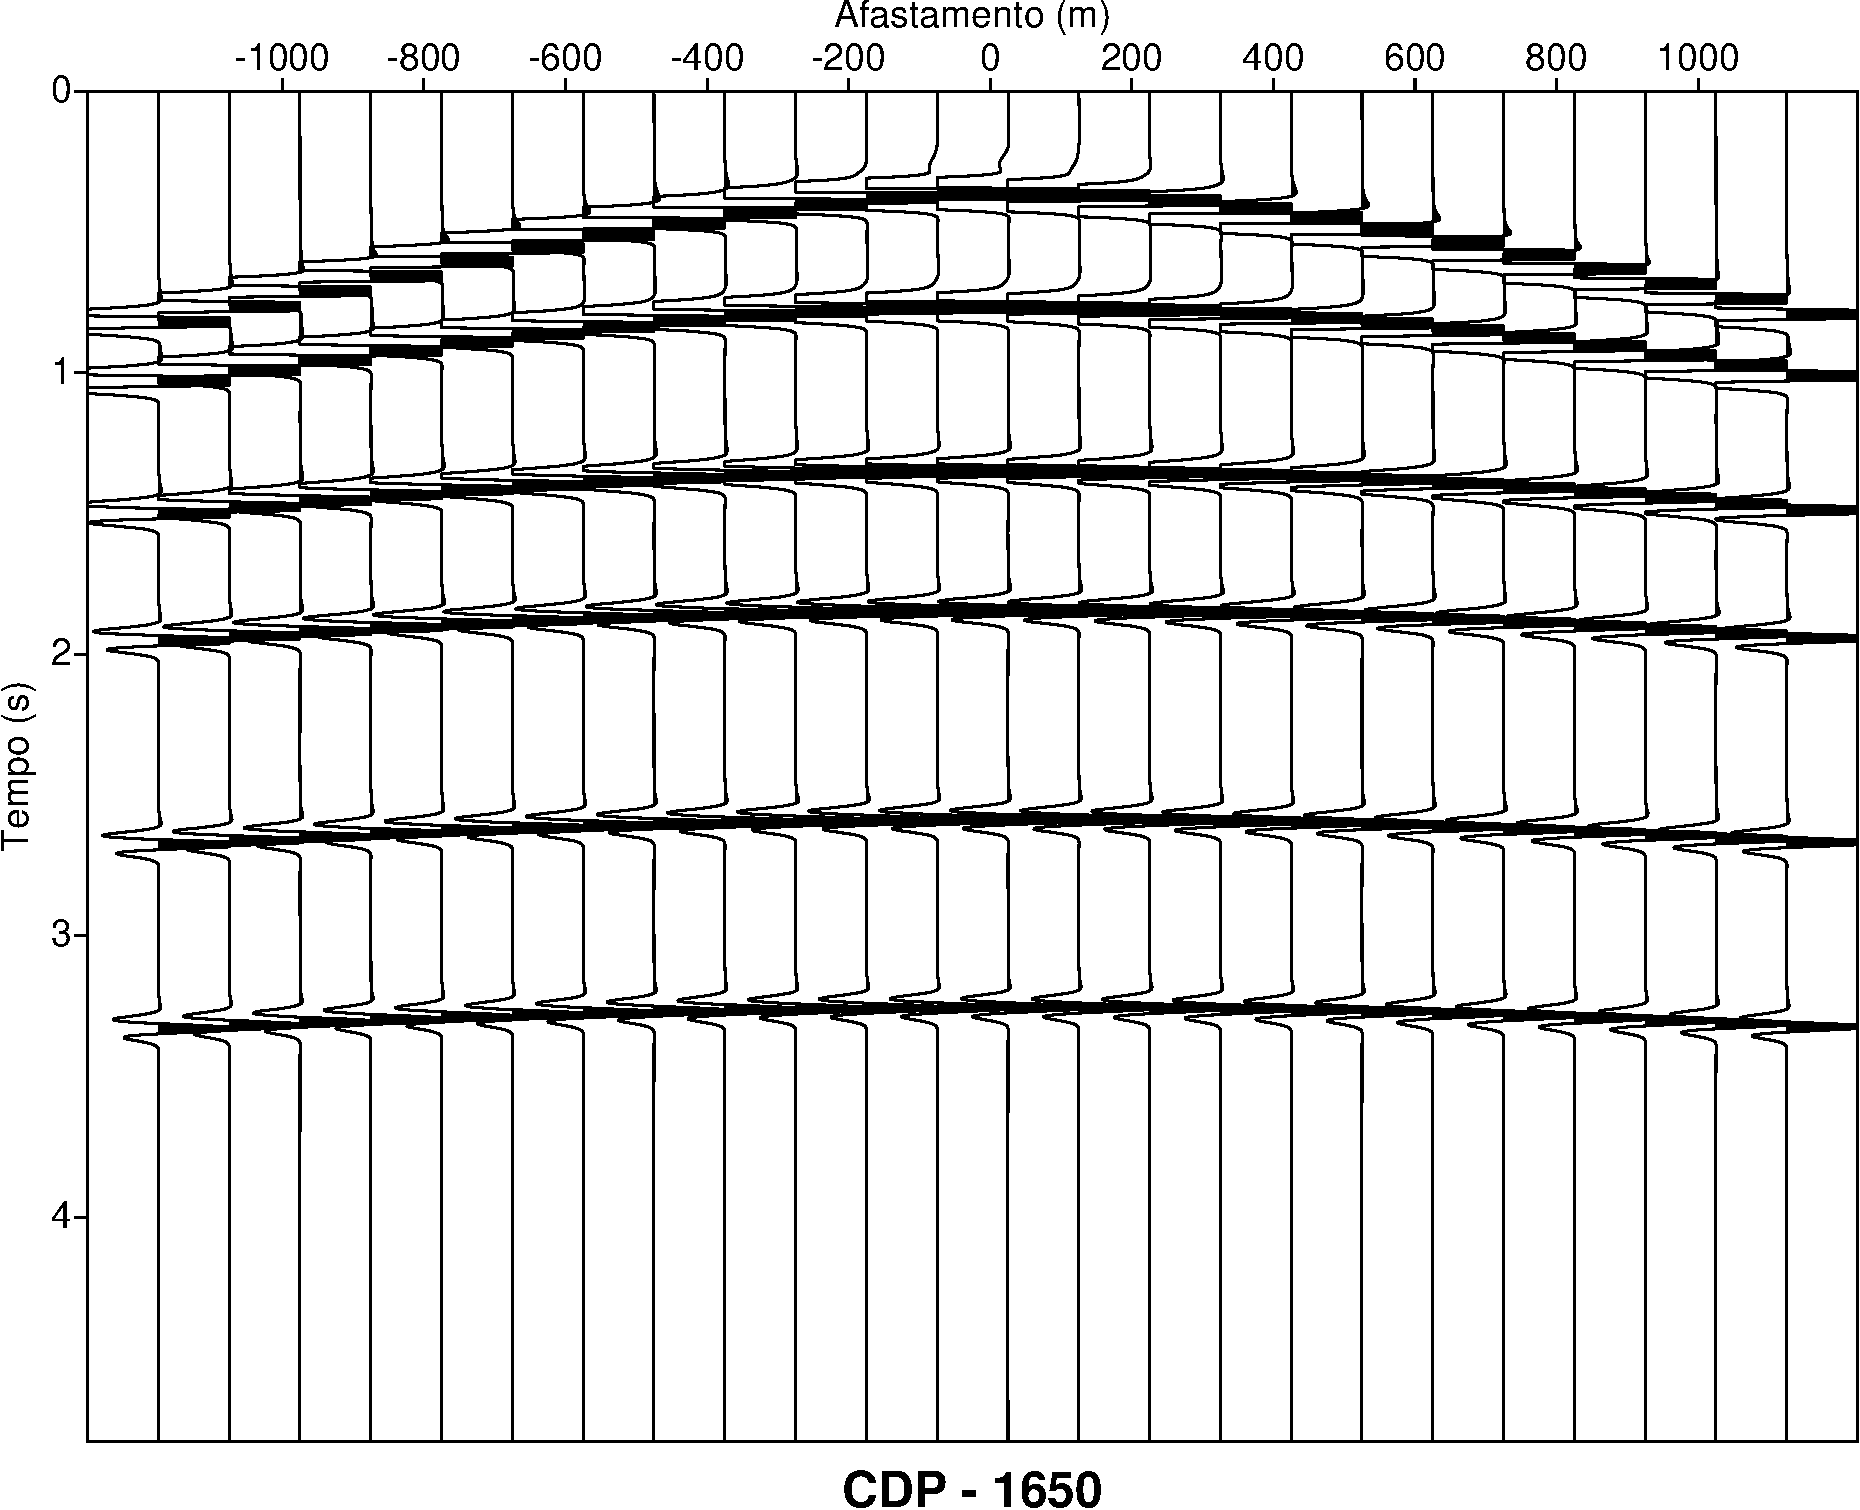
\includegraphics[width=12cm]{figuras/cap2/cmp1650.pdf}
        \caption{CDP - 1650}
        \label{fig:figure_a}
    \end{subfigure}%\hfill%
    \begin{subfigure}[b]{.80\textwidth}
        \centering
        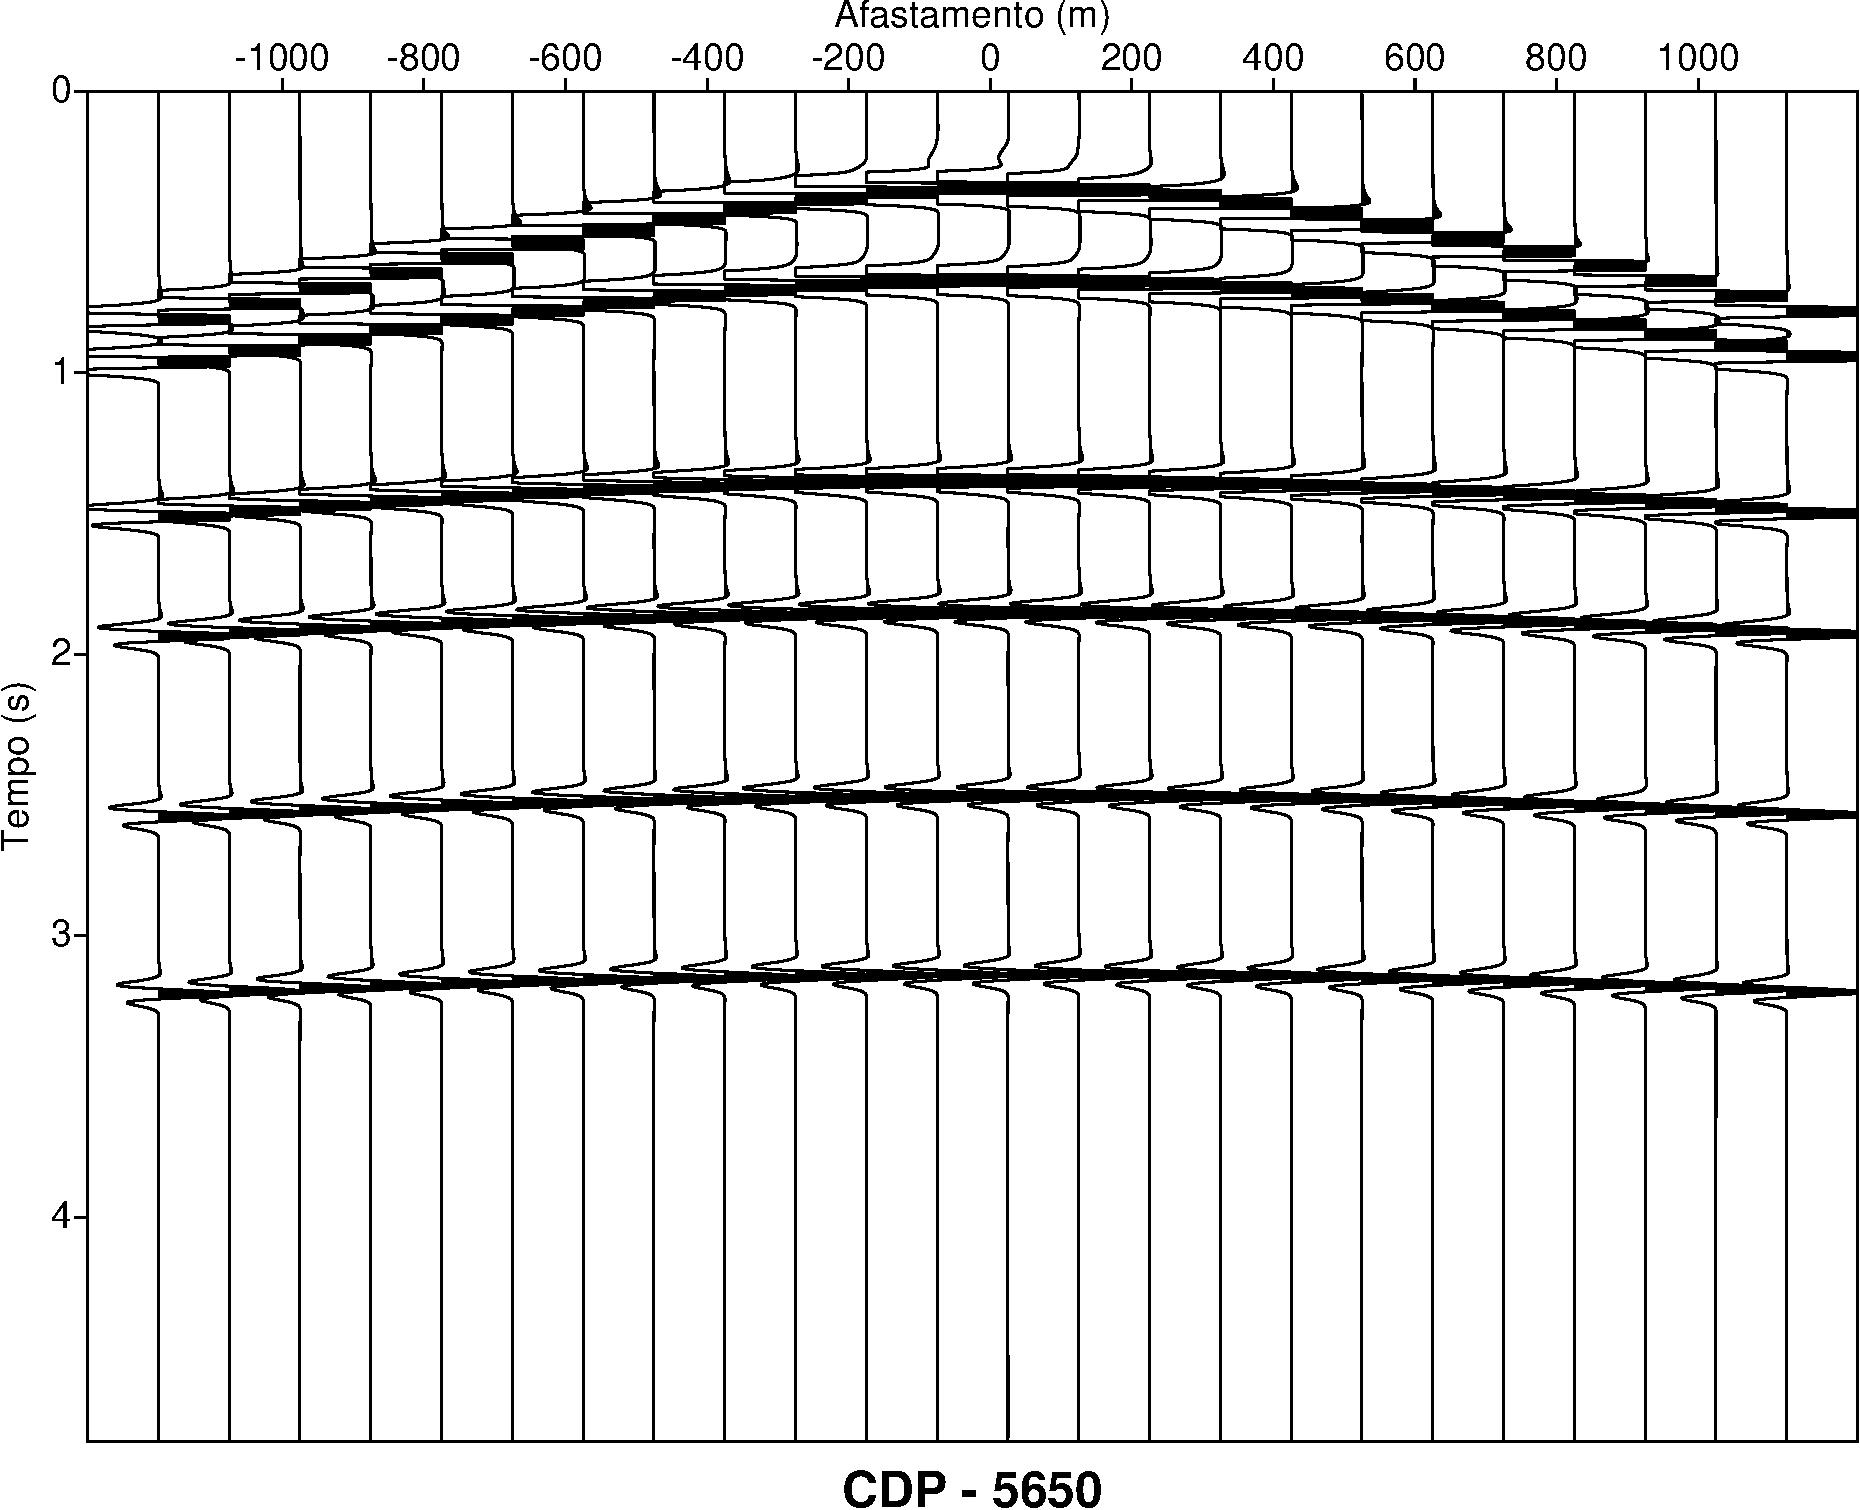
\includegraphics[width=12cm]{figuras/cap2/cmp5650.pdf}
        \caption{CDP - 5650}
        \label{fig:figure_b}
    \end{subfigure}
    \caption{CMP é um ponto em subsuperfície amostrado por diversos pares fonte-receptor. Esse conjunto de pares fonte-receptor recebe a denominação de família CDP ou CMP. A técnica foi inicialmente descrita para o caso de camadas horizontais plano-paralelas e com a velocidade do meio variando apenas no sentido vertical. Desde que foram estabelecidos no começo da década de 1950, os métodos common depth point (CDP), assim como os diferentes tipos de métodos de migração, são considerados a principal referência para o processamento de dados sísmicos.}
    \label{fig:fig_cdp1}
\end{figure}
\end{landscape}
\begin{landscape}
\begin{figure}[H]
    \centering
    \begin{subfigure}[b]{.80\textwidth}
        \centering
        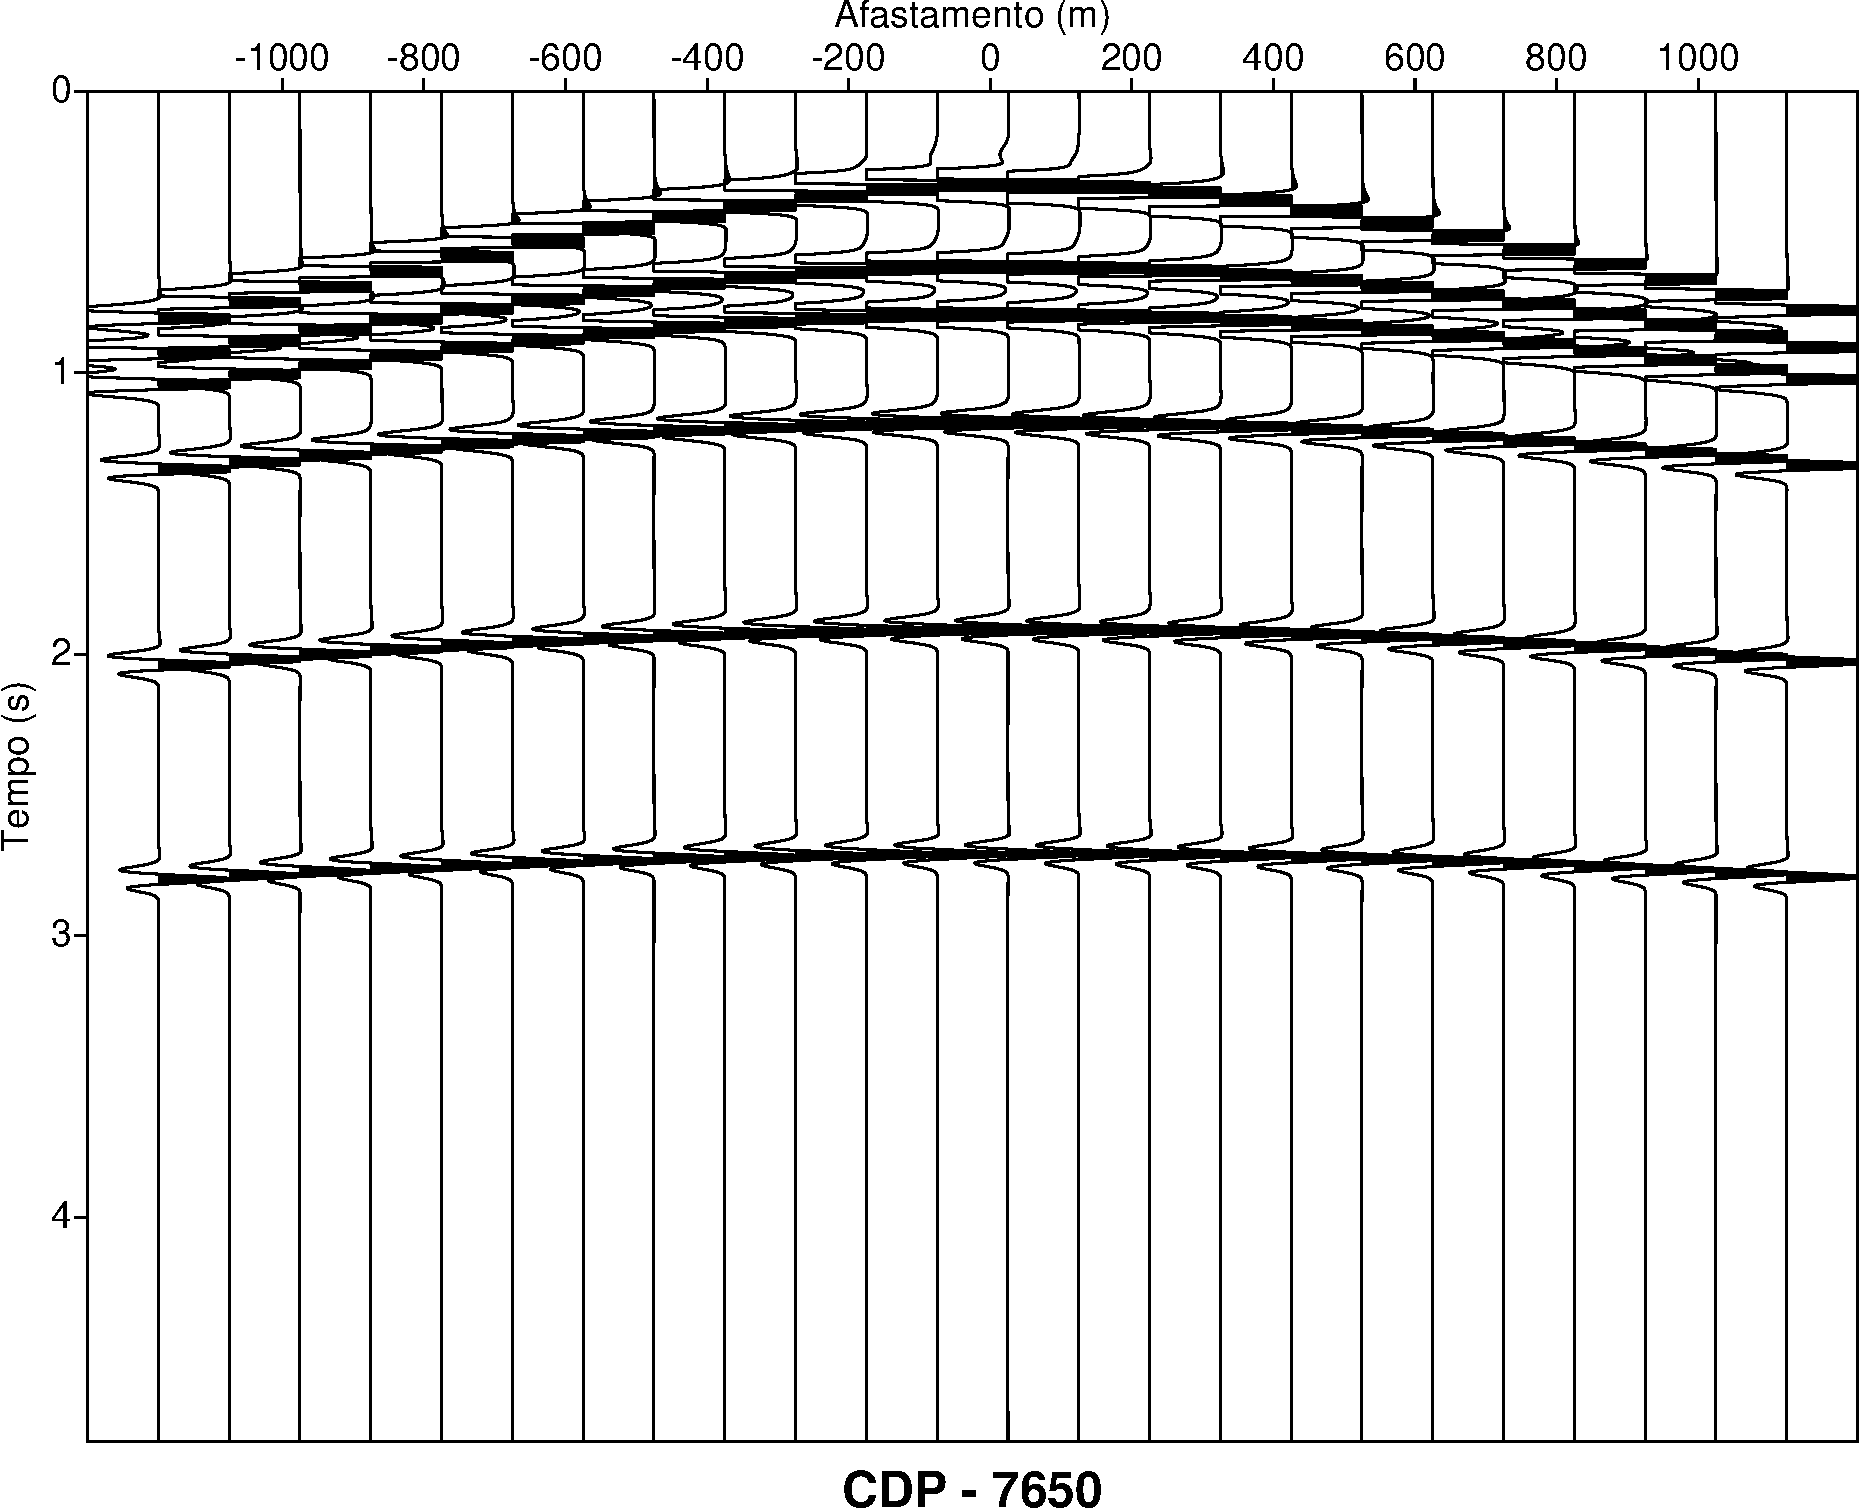
\includegraphics[width=12cm]{figuras/cap2/cmp7650.pdf}
        \caption{CDP - 7650}
        \label{fig:figure_c}
    \end{subfigure}%\hfill%
    \begin{subfigure}[b]{.80\textwidth}
        \centering
        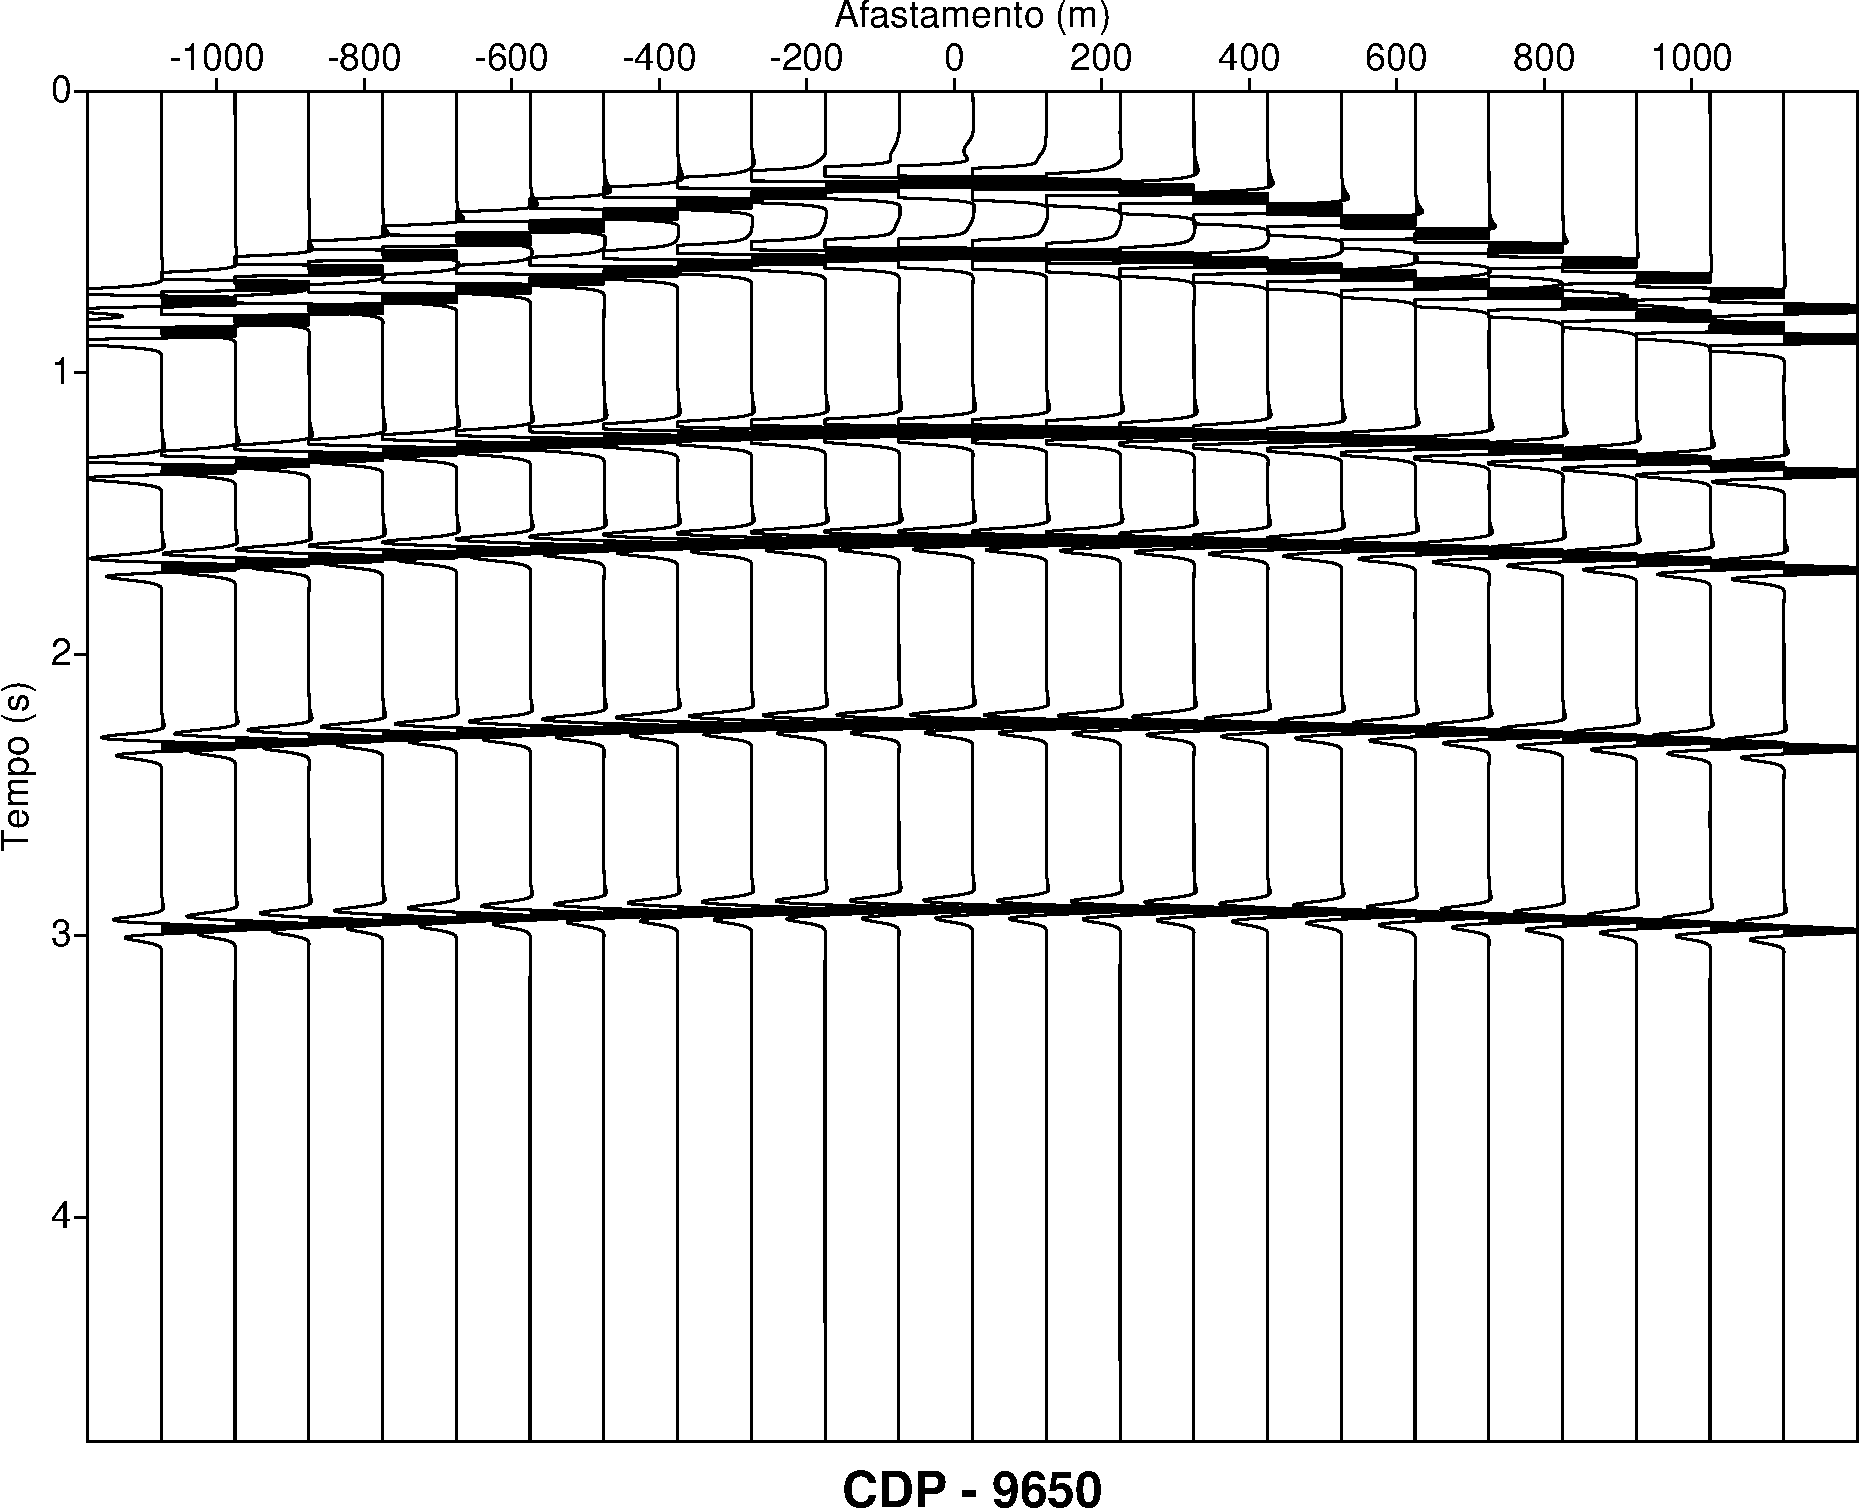
\includegraphics[width=12cm]{figuras/cap2/cmp9650.pdf}
        \caption{CDP - 9650}
        \label{fig:figure_d}
    \end{subfigure}
    \caption{A técnica CDP é uma maneira empregada em levantamento de reflexão sísmica para resolver
problemas de baixa qualidade do imageamento de áreas com baixa razão sinal/ruído. Nesta técnica
os pontos de subsuperfície são registrados redundantemente com diferentes afastamentos fonte-receptor.
A seção empilhada é obtida sobrepondo-se os traços redundantes, após a correção de sobre-tempo normal NMO.}
    \label{fig:fig_cdp2}
\end{figure}
\end{landscape}

\section{ANÁLISE DE VELOCIDADE E CORREÇÃO NMO}

A análise de velocidades é uma técnica que esta diretamente relacionada ao
sucesso do processamento sísmico. Quanto melhor for a estimativa do campo de
velocidades mais representativa será o imageamento da subsuperfície.

Há diversos tipos de velocidades definidas nos trabalhos sísmicos: velocidade
intervalar, velocidade RMS, velocidade de NMO e velocidade de empilhamento são
apenas algumas das mais importantes. Todas elas apresentam a sua importância,
porém a velocidade de empilhamento é a de maior importância no contexto de
análise de velocidade para imageamento.

Com o dado organizado em famílias CDP (figura \ref{fig:geometria_cdp}),
sabe-se que um CDP contém traços de um mesmo ponto de subsuperfície imageado várias vezes, com diferentes trajetos.
Então utilizando informações, do tempo de trânsito para os diferentes trajetos e o afastamento fonte - receptor, é
possível estimar a velocidade do meio. \citep{Yilmaz(2000)}.

A análise de velocidade não é realizada com apenas um CDP, e sim com um conjunto de
CDPs (CDPs de máxima cobertura) que são então interpoladas para os CDPs restantes.

A realização da análise de velocidade deve ser feita preferencialmente por um
intérprete. A etapa de picagem dos pontos envolve a seleção valores de velocidade
em função do tempo, para ser utilizada em processos subsequentes. Quando
realizada a análise de velocidade, busca-se sempre obter uma melhor imagem no
empilhamento, em que são tolerados erros na interpretação da velocidade. Assim,
precisa-se de bastante tempo para realizar essa tarefa, que apresenta grande
potencial para erros, especialmente quando o realizador da tarefa não conhece
muito a respeito da geologia do local.

A exatidão e resolução dos valores da velocidade de empilhamento dependem dos
fatores de aquisição do dado, tais como tamanho do afastamento (offset), cobertura, banda de
frequências da aquisição, razão sinal-ruído entre outros.

Para o trabalho em questão, algumas ferramentas foram utilizadas para auxiliar na
análise de velocidade. Estas ferramentas estão descritas a seguir.

A estimativa da distribuição de velocidade (modelo de velocidade) na seção sísmica usa o dado organizado em família CDP, a medida de coerência \textit{semblance},
faz-se a correção sobre-tempo-normal (NMO), realiza-se então o empilhamento da seção e posteriormente a aplica-se a técnica de migração.
A correção NMO é baseada no modelo de camada plano-horizontal, cujo tempo de trânsito de reflexão de uma onda primária tem forma hiperbólica definida pelo sobre-tempo-normal
em relação ao afastamento $x=0$, $\Delta t_{NMO}$, e expressa por:
\begin{eqnarray}
\Delta t_{NMO}(h,t(0),v_{NMO})=t(x)-t(0);
\label{t_NMO}
\end{eqnarray}
que a partir da Eq. (\ref{eq:tempo_de_transito}) fica na forma:
\begin{eqnarray}
\Delta t_{NMO}(h,t(0),v_{NMO})=t(0)\left\lbrace \left[ 1 + \left( \frac{x}{t(0)v_{NMO}}\right)^2\right]^{\frac{1}{2}}-1\right\rbrace.
\label{t_NMO_2}
\end{eqnarray}

Na aplicação de $\Delta t_{NMO}$ se busca a horizontalizar os eventos hiperbólicos em relação à $t(0)$ ajustando o parâmetro $v_{NMO}$. A estimativa de velocidade é realizada acoplada ao mapa semblance, $S(v_{NMO},t_0;x_0)$, que mede a coerência no intervalo $[0,1]$, e é dada por \citep{Sguazzero(1987)}:
\begin{eqnarray}
S\left(v_{NMO}, t_{0} ; x_{0}\right)=\frac{\displaystyle\sum_{t=t_{0}-\delta t / 2}^{t_{0}+\delta t / 2}\left[\frac{1}{N_{h}}\displaystyle\sum_{h=h_{0}}^{\delta h} \bar{u}\left[t\left(h, v_{N M O}\right) ; x_{0}\right]\right]^{2}}{\displaystyle\sum_{t=t_{0}+\delta t / 2}^{t_{0}+\delta t / 2} \frac{1}{N_{h}}\displaystyle\sum_{h=h_{0}}^{\delta h}\left[\bar{u}\left[t\left(h, v_{N M O}\right) ; x_{0}\right]\right]^{2}},
\label{eq:semblance}
\end{eqnarray}
onde $\bar{u}[t(h,v_{NMO});x_0]$ \'e a amplitude do tra\c{c}o ao longo da trajetória de empilhamento, $\sum_t$ e $\sum_h$ definem as janelas temporal-espacial dentro da qual se ajusta a curva que melhor representa o evento de reflex\~ao, e $N_h$ é o número de traços envolvidos. Os pares ($v_{NMO},t_0$) devem ser marcados no mapa semblance em conjunto com a an\'alise dos eventos de reflexão, e cada evento é relacionado a um par que melhor o horizontaliza (ver figura \ref{fig:correcao_nmo}), assim se forma o modelo de velocidades NMO utilizado, primeiramente, no empilhamento e, posteriormente, na migração.

Para o dado de arranjo split-spread, a análise de velocidade foi feita em 18 CDPs (1150, 1650, 2150, 2650, 3150, 3650, 4150, 4650, 5150, 5650, 6150, 6650, 7150, 7650, 8150, 8650, 9150, e 9650), ou seja, a partir do CDP de cobertura máxima 1150 foi dado um espaçamento regular de 500 CDPs até chegar ao CDP 9650, pois o CDP 10788 (último CDP de cobertura máxima) não está incluso para este intervalo.

Para cada CDP é gerado um semblance (medida de coerência multicanal), \citep{Sheriff(1995)}, onde as regiões em vermelho representam as velocidades mais coerentes para horizontalizar os refletores. Sendo assim, o usuário deve apontar o cursor do mouse na região onde achar que corresponde a velocidade mais representativa, e pressionar a letra ``s'' no teclado. Este comando salvará os picks correspondentes aos pares de velocidades $v_{NMO}$ e tempos $t_{NMO}$.

Em seguida, depois de ter salvado todos os picks de um determinado CDP é necessário pressionar a tecla ``q'', para finalizar o processo de picagem.

Após o processo de picagem onde escolhe-se os pares de velocidades $v_{NMO}$ e tempos $t_{NMO}$ pode-se então aplicar a correção de sobre-tempo-normal. O programa que realiza a correção de NMO no SU em um dado sísmico é o sunmo (ver anexo). Os parâmetros de entrada para a correção NMO no SU são os seguintes:

\begin{itemize}
 \item $t_{NMO}$ - Tempo NMO correspondente para velocidades $v_{NMO}$.
 \item $v_{NMO}$ - velocidades NMO correspondentes aos tempo $t_{NMO}$.
 \item $CDP$ - CDPs para os quais $v_{NMO}$ e $t_{NMO}$ são especificados.
\end{itemize}


\begin{figure}[H]
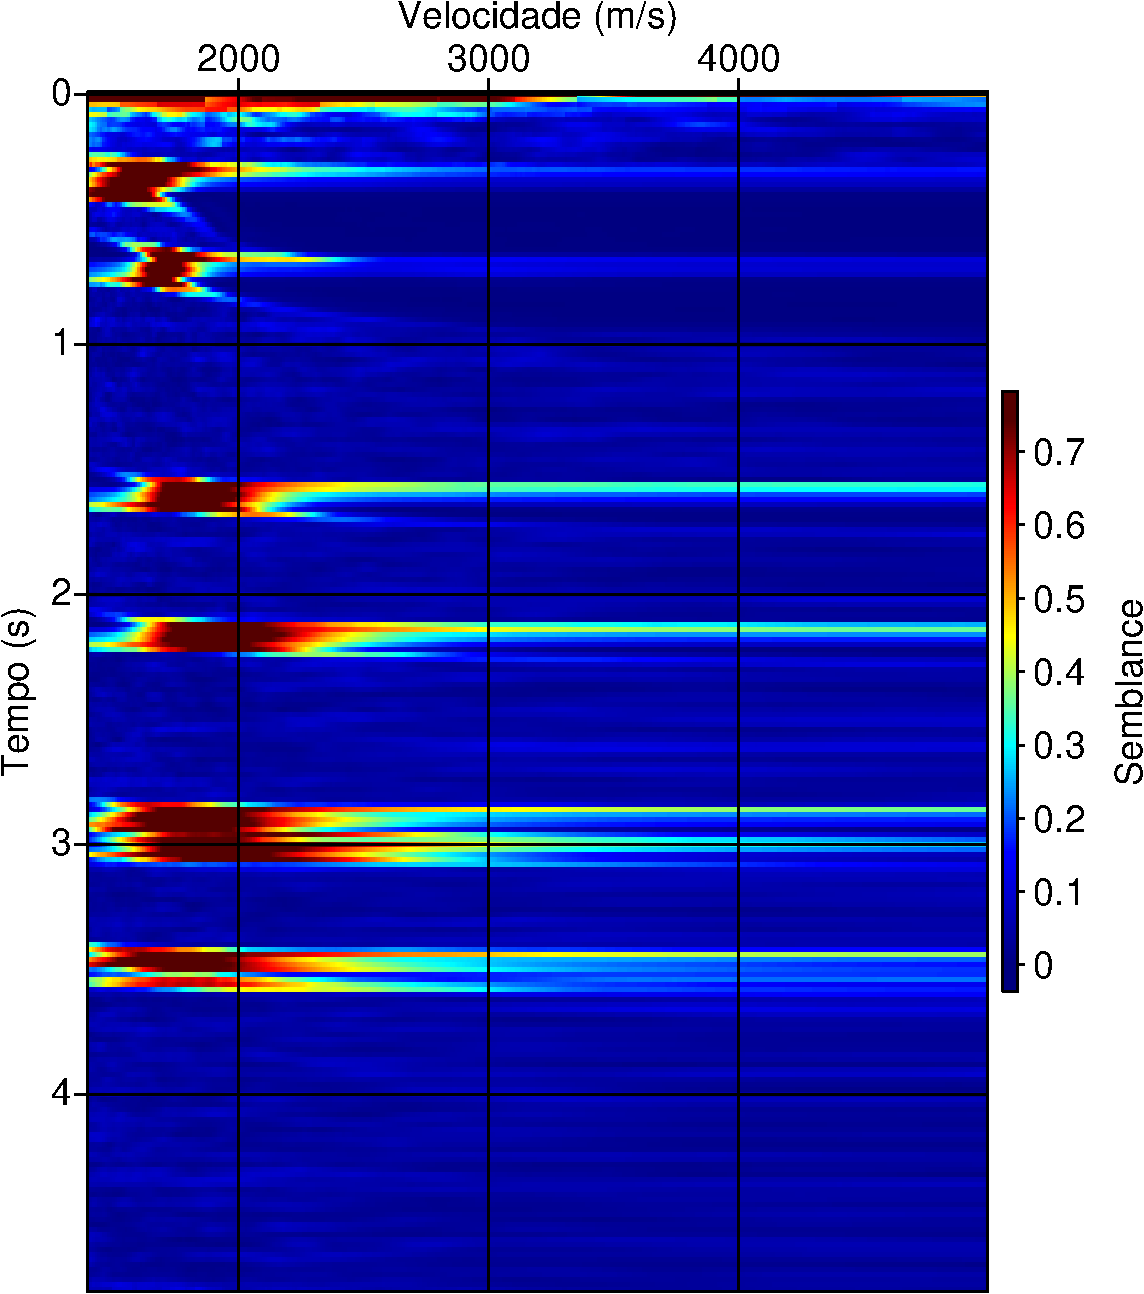
\includegraphics[width=5cm,height=7cm]{figuras/cap2/Semblance_color_4650.pdf}
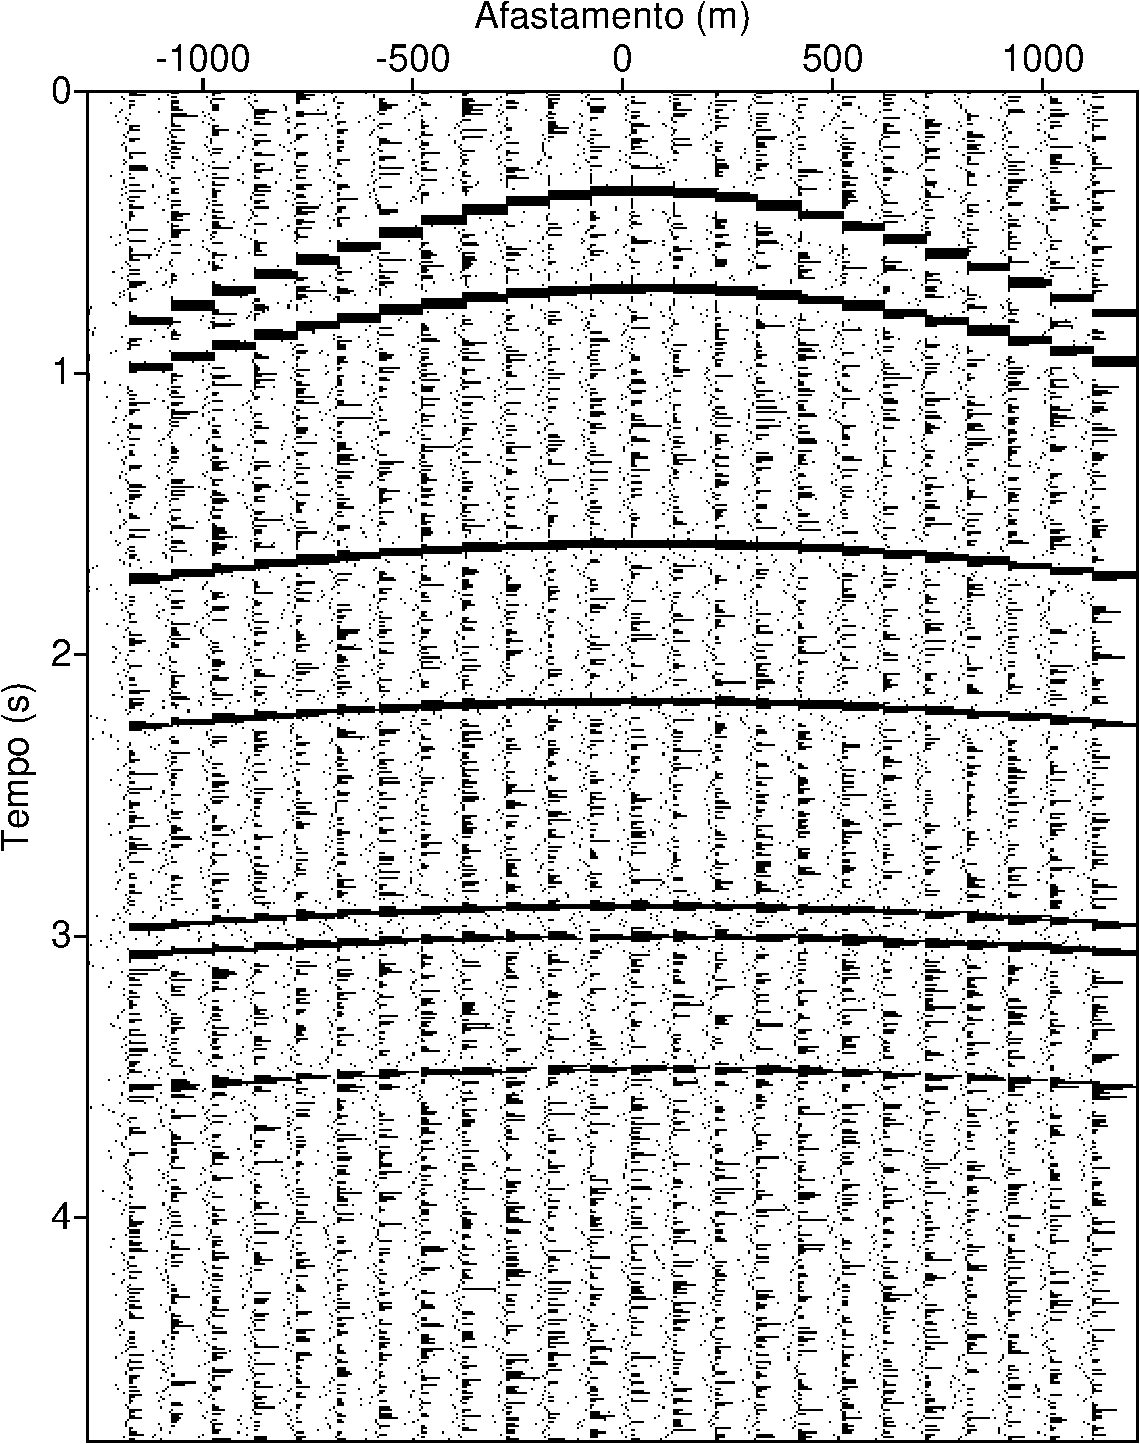
\includegraphics[width=5cm,height=7cm]{figuras/cap2/CMP_4650.pdf}
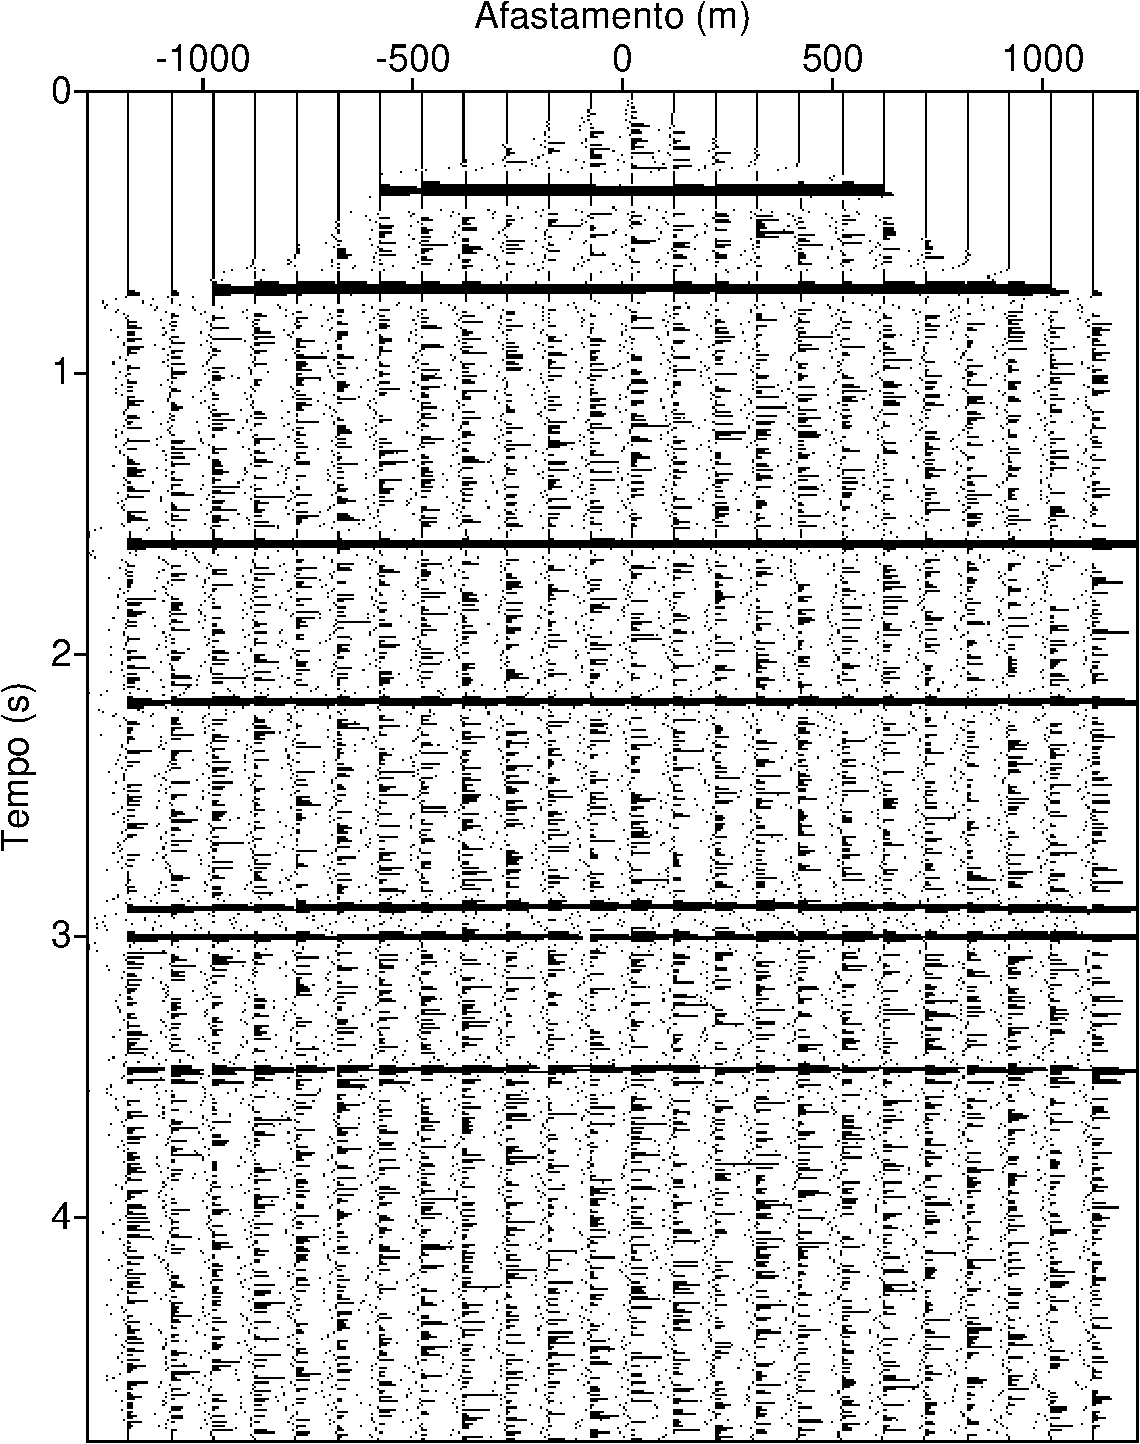
\includegraphics[width=5cm,height=7cm]{figuras/cap2/CMP_After_NMO_4650.pdf}
\caption{CMP - 4650: mapa semblance (à esquerda), antes da correção NMO (centro) e após a correção NMO (à direita).}
\label{fig:correcao_nmo}
\end{figure}

% \begin{figure}[H]
%   \centering
%   \begin{subfigure}{.3\linewidth}
%     \centering
%     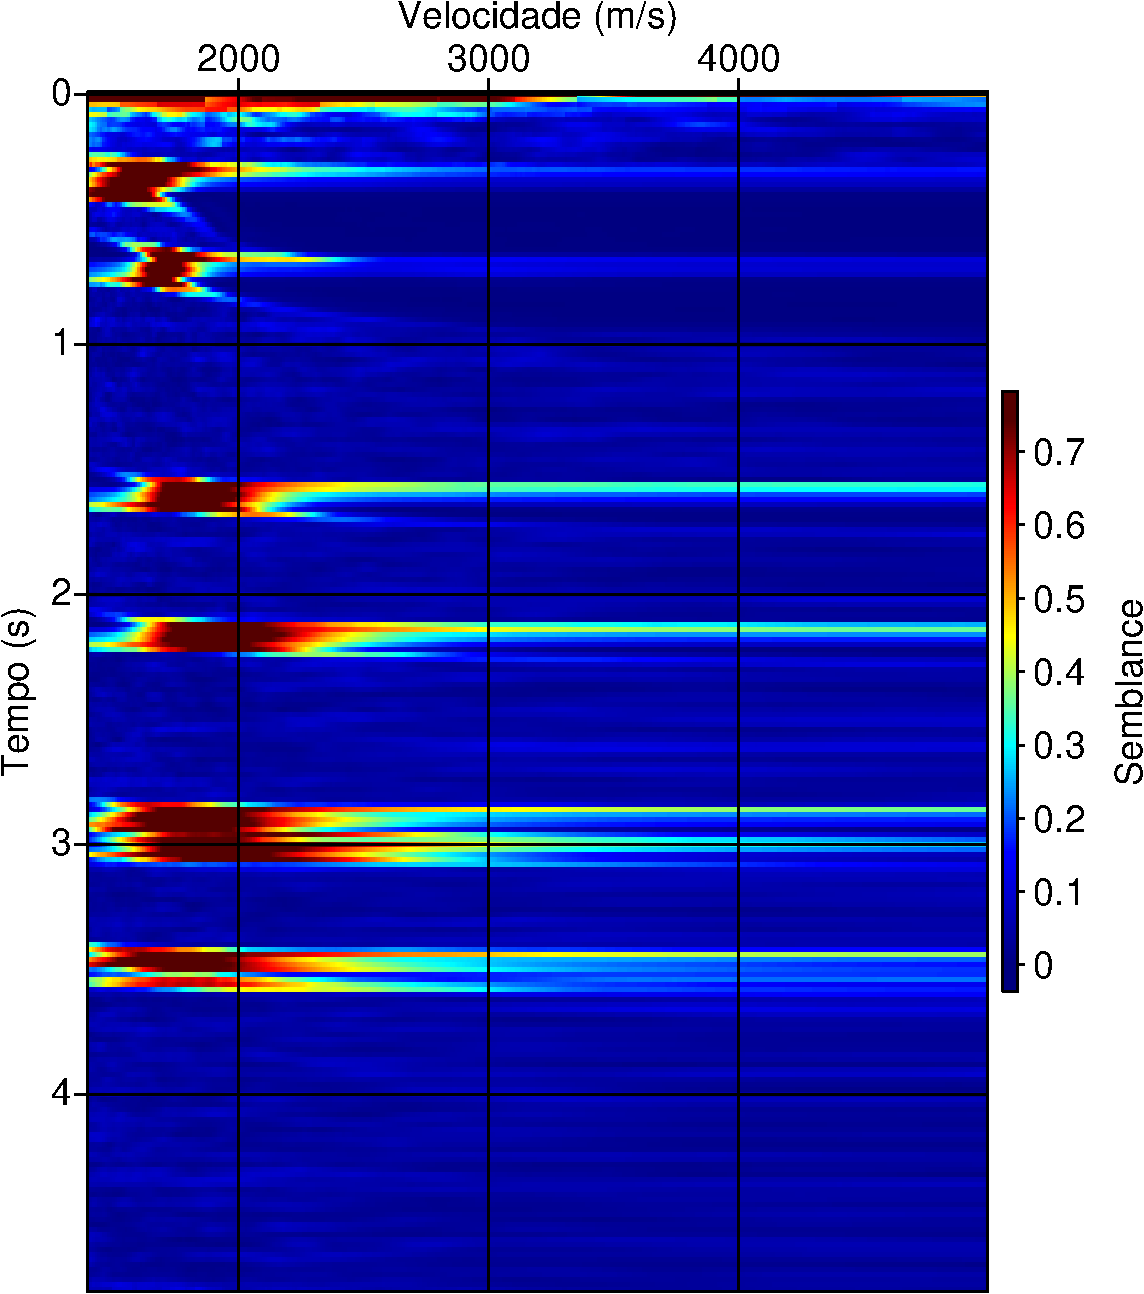
\includegraphics[width = \linewidth,height=7cm]{figuras/cap2/Semblance_color_4650.pdf}
%     \caption{Mapa semblance}
%   \end{subfigure}%
%   \hspace{1em}% Space between image A and B
%   \begin{subfigure}{.3\linewidth}
%     \centering
%     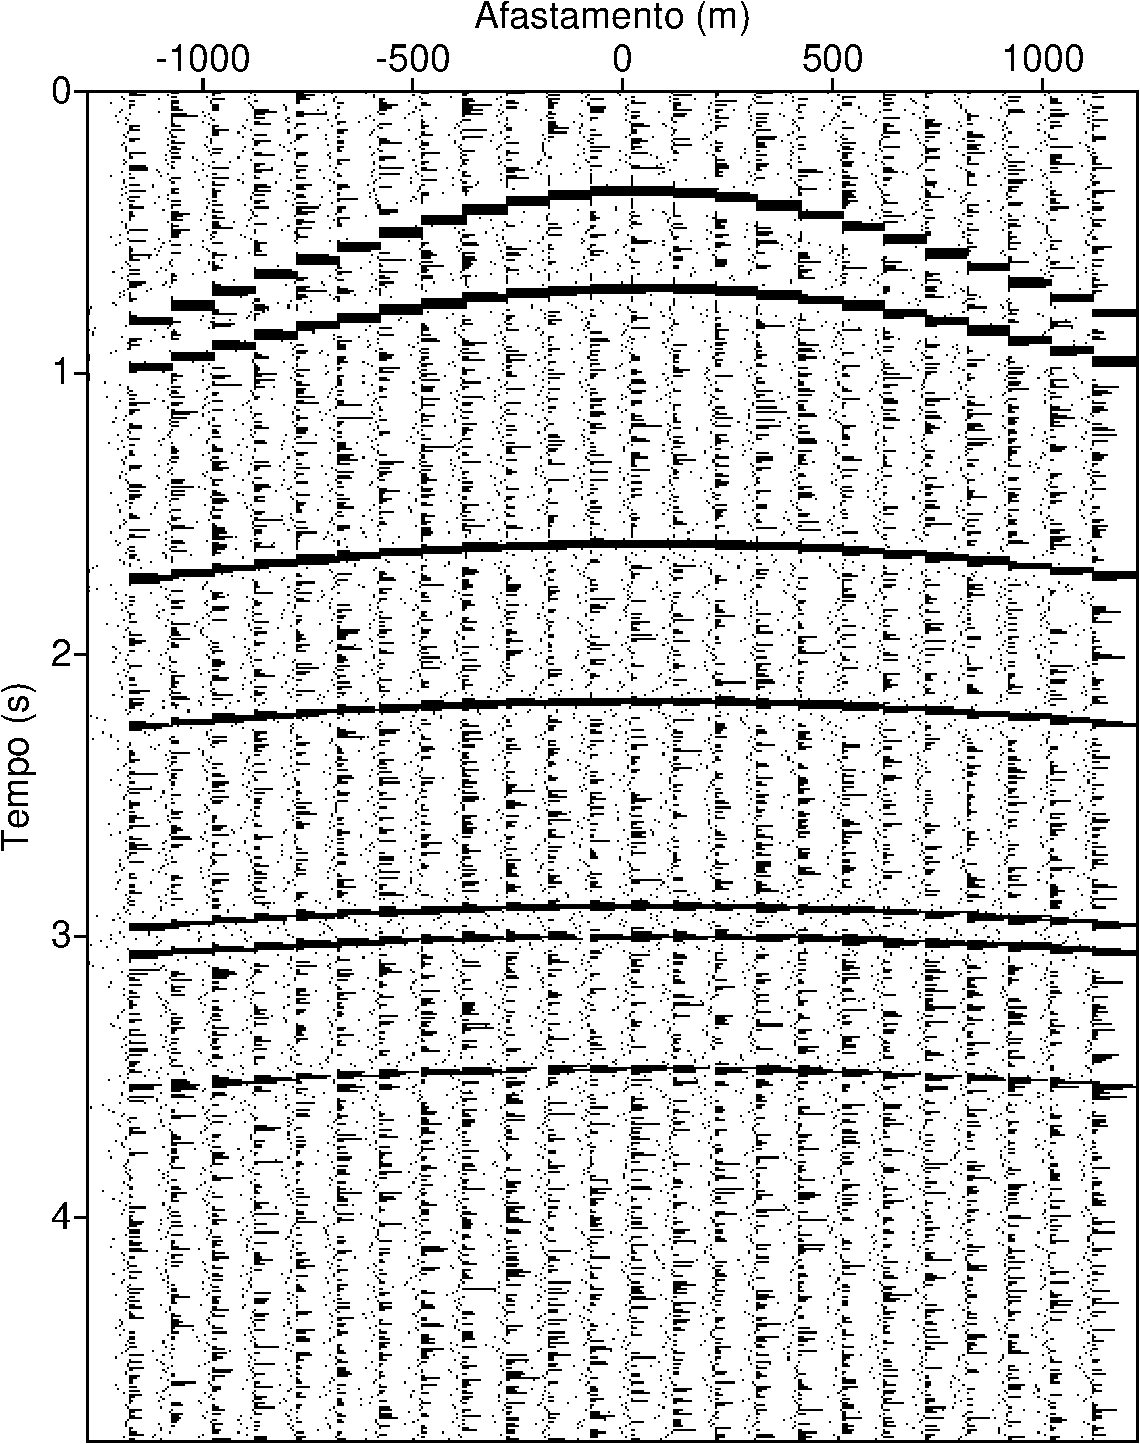
\includegraphics[width = \linewidth,height=7cm]{figuras/cap2/CMP_4650.pdf}
%     \caption{CDP 4650 antes da correção NMO}
%   \end{subfigure}%
%   \hspace{1em}% Space between image B and C
%   \begin{subfigure}{.3\linewidth}
%     \centering
%     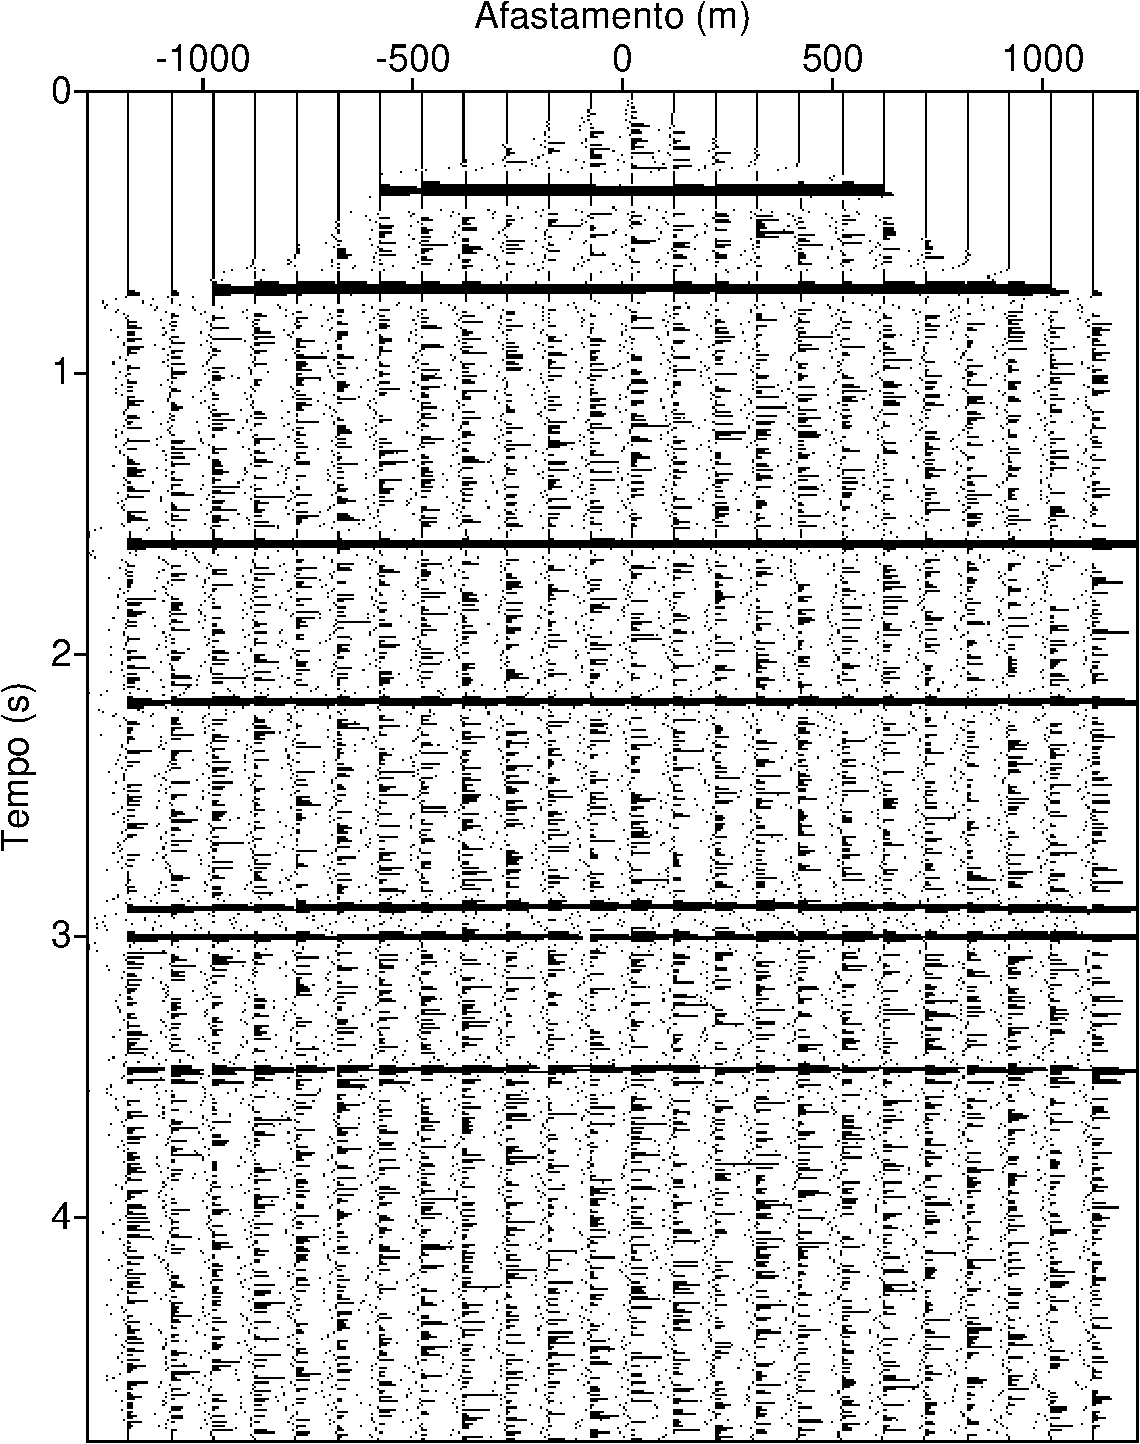
\includegraphics[width = \linewidth,height=7cm]{figuras/cap2/CMP_After_NMO_4650.pdf}
%     \caption{CDP 4650 depois da correção NMO}
%   \end{subfigure}
%   \caption{CMP 4650}
%   \label{fig:correcao_nmo}
% \end{figure}

 Conhecido os pares de velocidades $v_{NMO}$ e tempos $t_{NMO}$ de todos os CDPs analisados no processo de picagem gera-se os modelos de velocidade NMO (ver anexo). A figura \ref{fig:campovel2} e figura \ref{fig:campovel_suavizado} mostram respectivamente os modelos de velocidade NMO e velocidade NMO suavizado em tempo utilizado no empilhamento do dado. 

\begin{landscape}
\begin{figure}[H]
\centering
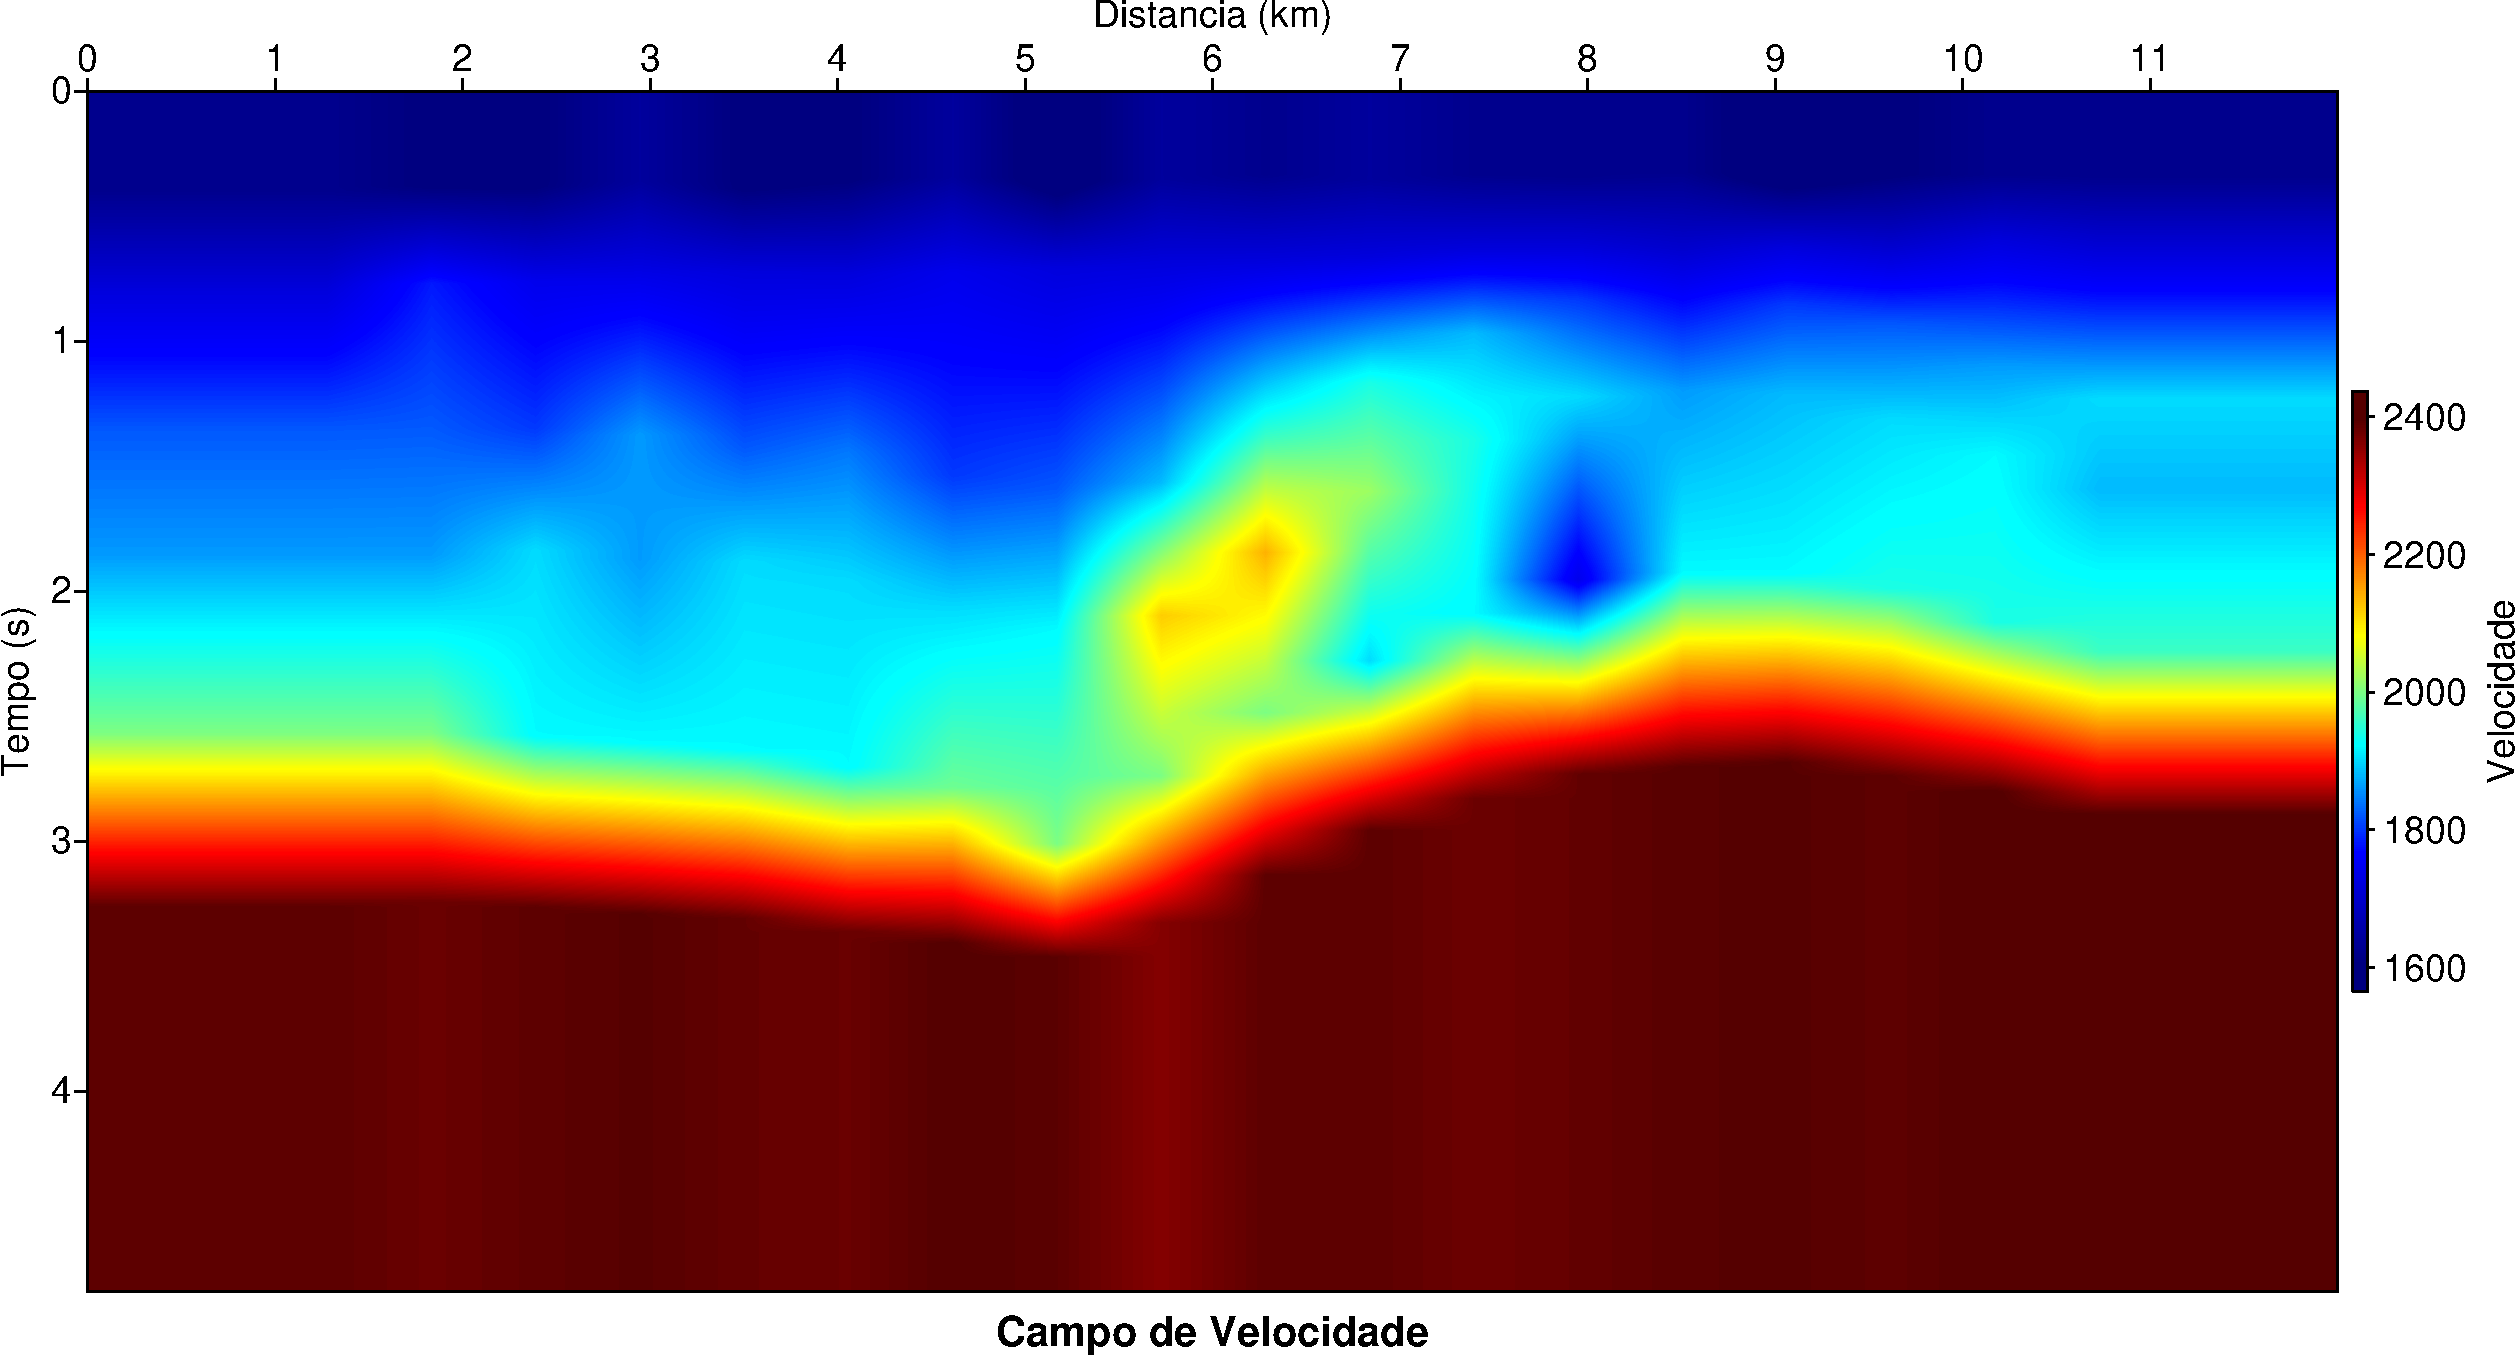
\includegraphics[totalheight=14cm]{figuras/cap2/campovel2.pdf}
\caption{Modelo de velocidade em tempo não suavizado obtido no SU. A cor azul escuro está relacionada as camadas de baixas velocidades e a cor vermelha escura as camadas de altas velocidades (camadas mais próximas do embasamento consequentemente mais profundas).}
\label{fig:campovel2}
\end{figure}
\end{landscape}

\begin{landscape}
\begin{figure}[H]
\centering
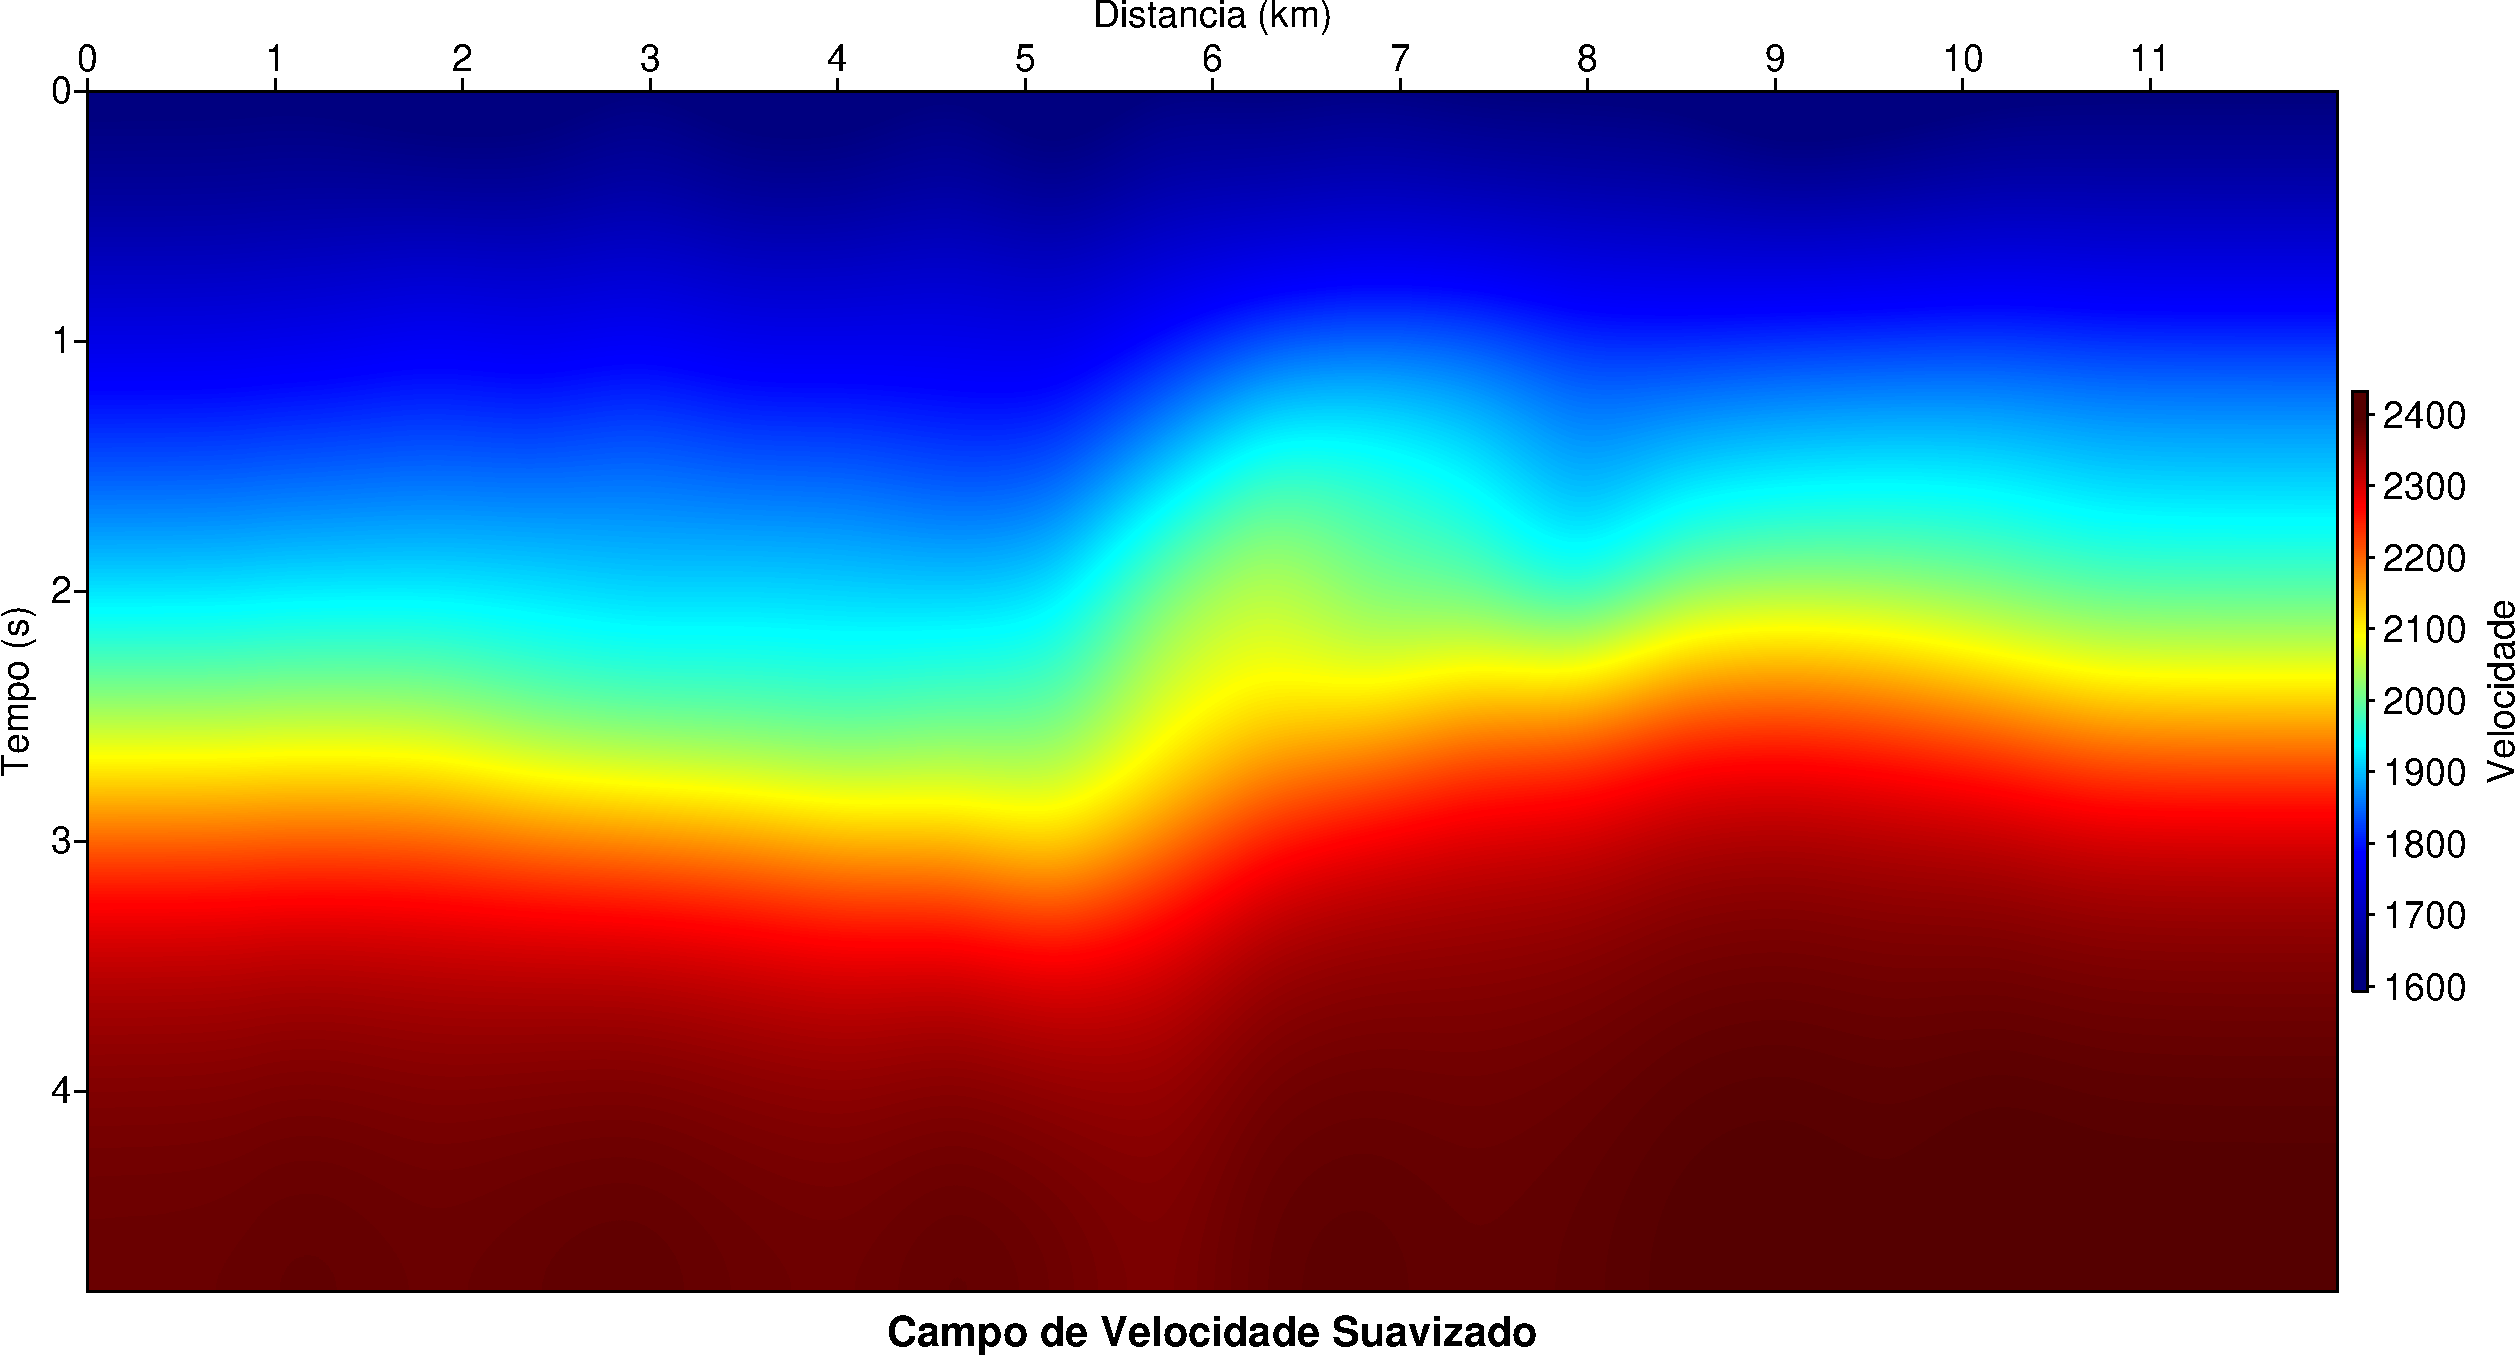
\includegraphics[totalheight=14cm]{figuras/cap2/campovel_suavizado.pdf}
\caption{Modelo de velocidade em tempo suavizado obtido no SU. A cor azul escuro está relacionada as camadas de baixas velocidades e a cor vermelha escura as camadas de altas velocidades (camadas mais próximas do embasamento consequentemente mais profundas).}
\label{fig:campovel_suavizado}
\end{figure}
\end{landscape}

\section{EMPILHAMENTO}

O objetivo do empilhamento sísmico é simular um experimento sísmico de incidência normal, ou seja simular uma aquisição onde fonte e receptores (geofones) estivessem na mesma posição, este procedimento só é possível quando o dado de entrada esta organizado em família CDP. O empilhamento sísmico consiste na soma de todos os traços das famílias CDP, após a correção de NMO, que gerará um traço resultante. Essa etapa é realizada após a correção de NMO para que os eventos estejam horizontalizados e possam ser somados de forma construtiva. A soma construtiva recebe o nome de STACK e a imagem obtida é
chamada de seção empilhada. \citep{Vasconcellos(2009)}

Para que os traços da seção obtenham maior coerência dos eventos registrados o valor da amplitude somada e dividida pelo número de traços. 
Os primeiros eventos são somados em fase (construtivamente) e os outros eventos coerentes (ruídos) serão somados de forma destrutiva.
Através do processo de empilhamento o ruído aleatório é atenuado em $\sqrt{N}$, onde $N$ é o número de canais empilhados em conjunto.

\begin{figure}[H]
\centering
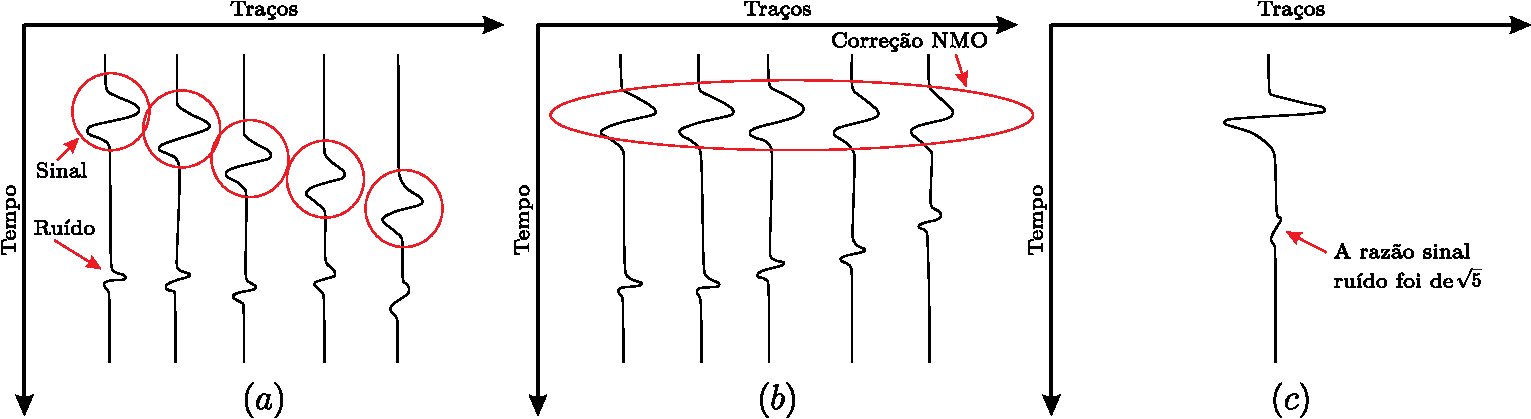
\includegraphics[width=16cm]{figuras/cap2/empilhamento.pdf}
\caption{a) Cinco canais antes do empilhamento com ruído, b) Os cinco canais após a correção NMO, c) Canais já empilhados e com atenuação do ruído de $\sqrt{N}$. Onde $N$ é o no de canais. Figura adaptada de \citep{Vasconcellos(2009)}}
\label{fig:empilhamento}
\end{figure}

\begin{landscape}
\begin{figure}[H]
\centering
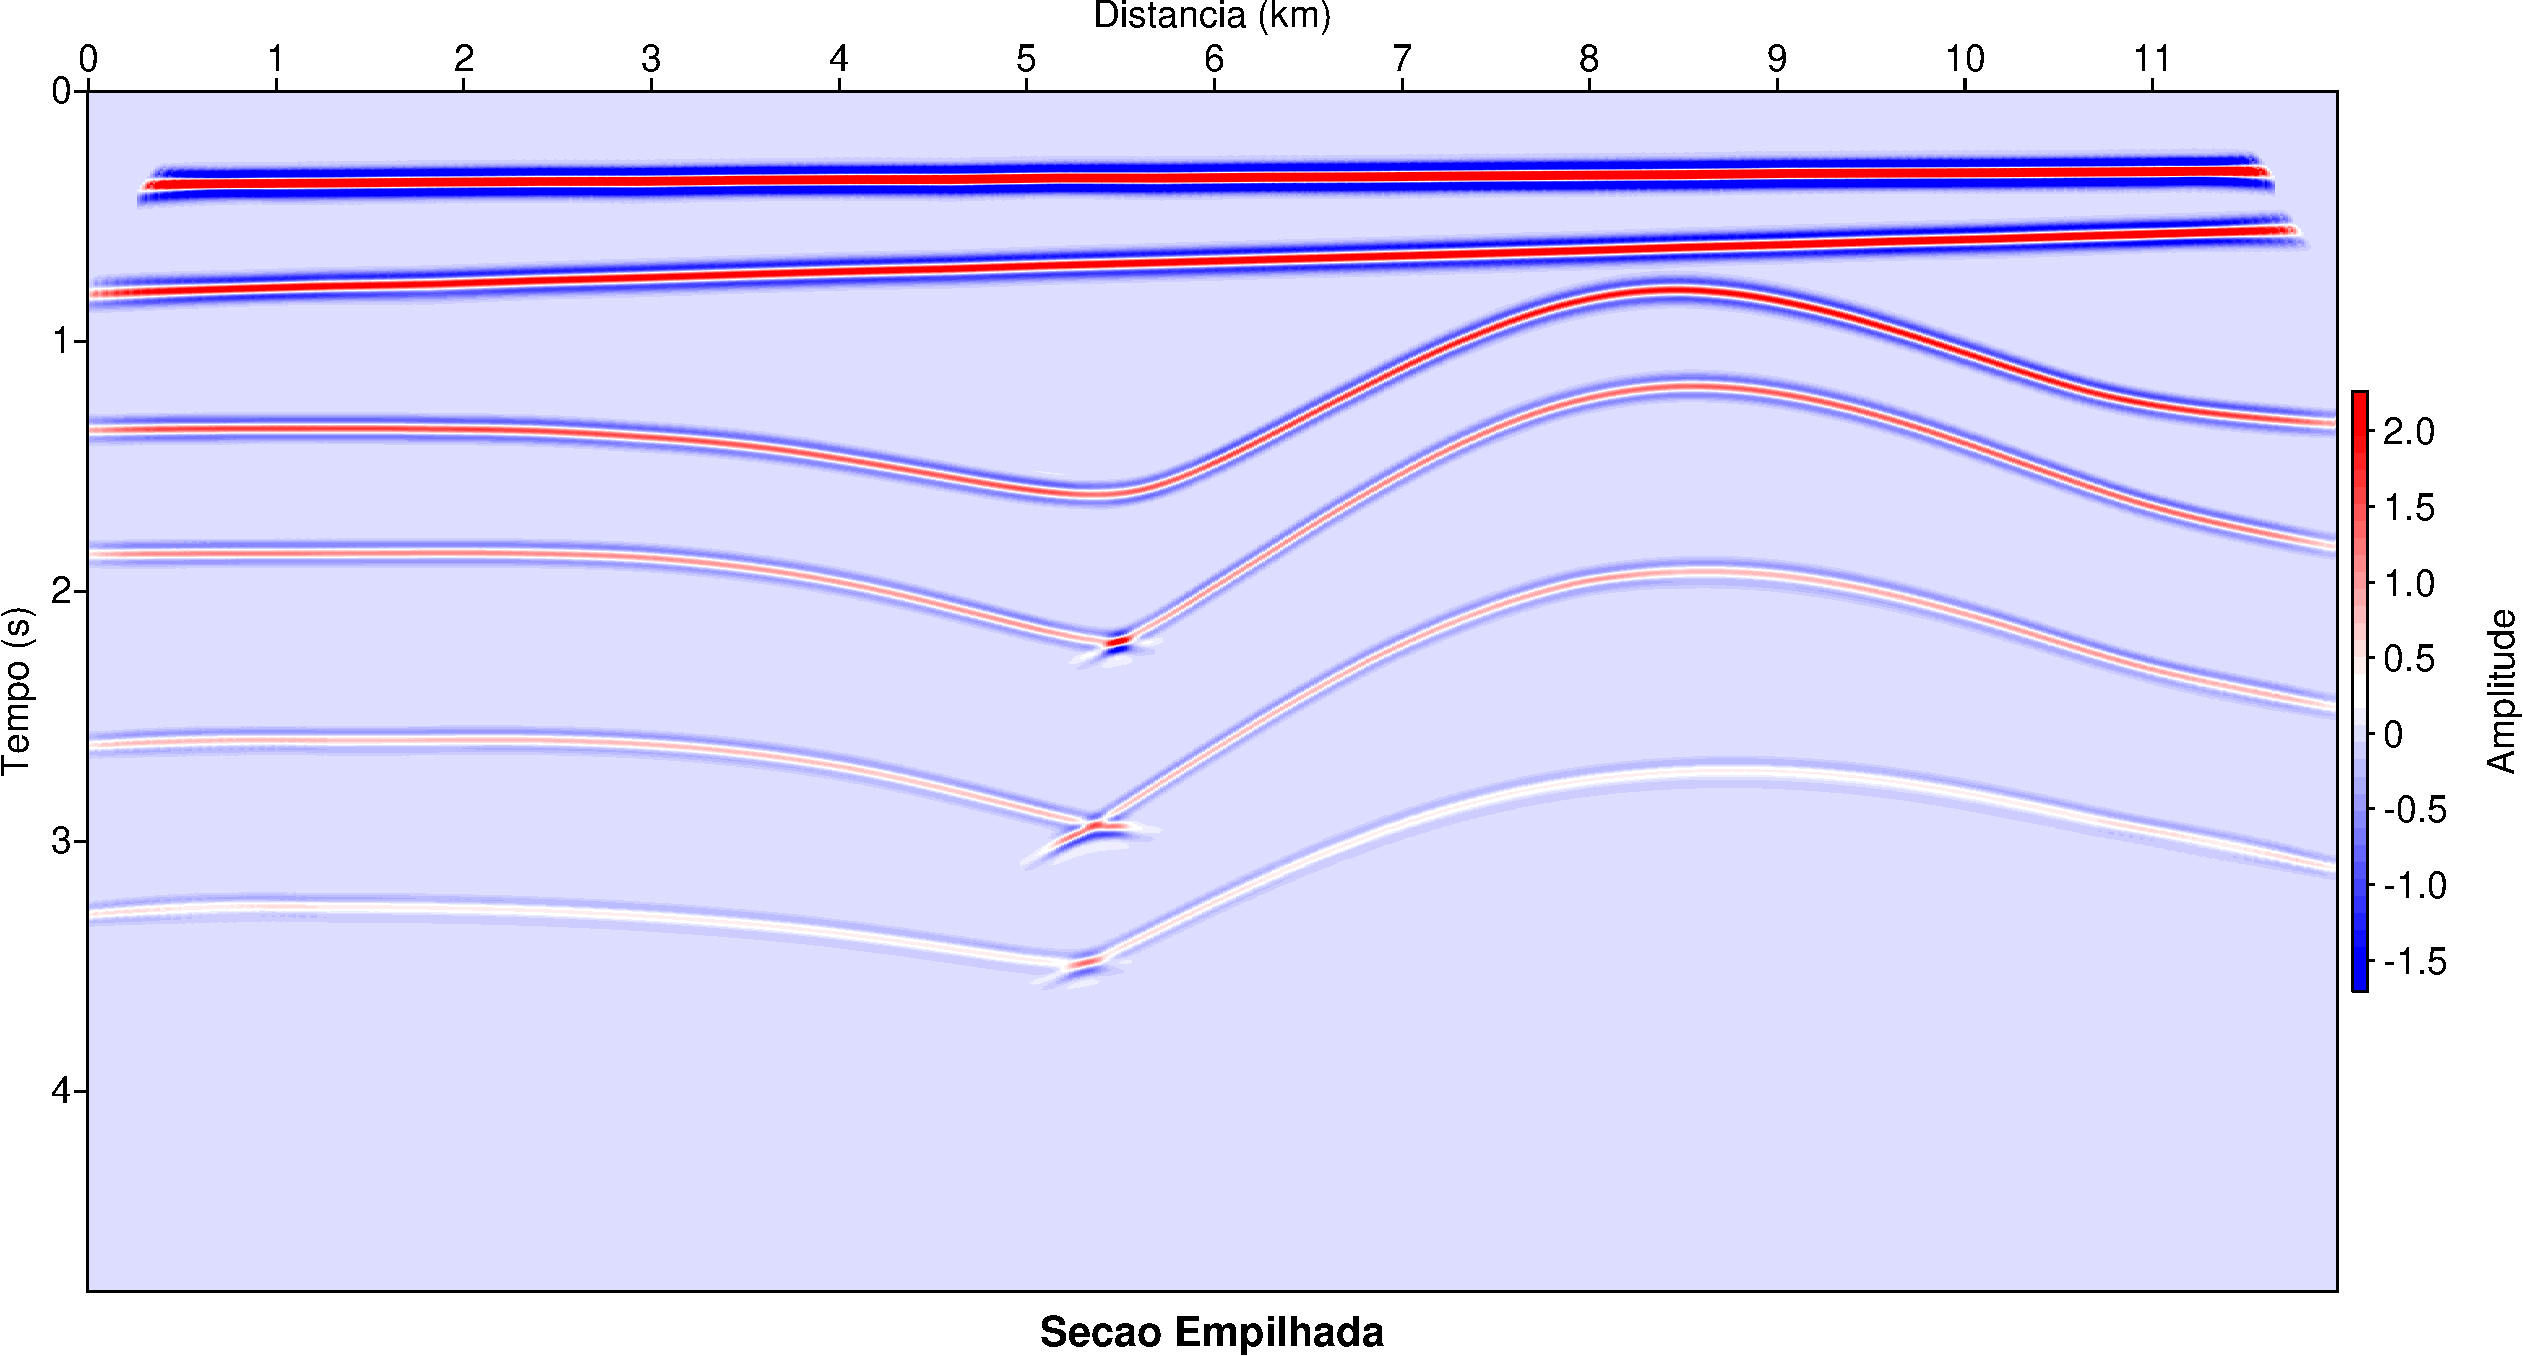
\includegraphics[totalheight=14cm]{figuras/cap2/seis_stack.pdf}
\caption{Seção empilhada}
\label{fig:seis_stack}
\end{figure}
\end{landscape}
